%================================================================
% SLO
%----------------------------------------------------------------
% datoteka: 	thesis_template.tex
%
% opis: 		predloga za pisanje diplomskega dela v formatu LaTeX na
% 				Univerza v Ljubljani, Fakulteti za računalništvo in informatiko
%
% pripravili: 	Matej Kristan, Zoran Bosnić, Andrej Čopar,
%			  	po začetni predlogi Gašperja Fijavža
%
% popravil: 	Domen Rački, Jaka Cikač, Matej Kristan
%
% verzija: 		30. september 2016 (dodan razširjeni povzetek)
%================================================================


%================================================================
% SLO: definiraj strukturo dokumenta
% ENG: define file structure
%================================================================
\documentclass[a4paper, 12pt]{book}
\usepackage{longtable}
\usepackage{multirow}


%================================================================
% SLO: Odkomentiraj "\SLOtrue " za izbiro slovenskega jezika
% ENG: Uncomment "\SLOfalse" to chose English languagge
%================================================================
\newif\ifSLO
% switch language

\SLOtrue % Enables Slovenian language
%\SLOfalse  % Enables English language

%================================================================
% SLO: vključi oblikovanje in pakete
% ENG: include design and packages
%================================================================
%----------------------------------------------------------------
% SLO: LaTeX paketi
% ENG: LateX packages
%----------------------------------------------------------------
% SLO: omogoča uporabo slovenskih (latinskih) črk kodiranih v formatu UTF-8
% ENG: enables the use of slovene (latin) caracters encoded in the UFT-8 format
\usepackage[utf8x]{inputenc}
%\inputencoding{utf8} 
% SLO: naloži, med drugim, slovenske delilne vzorce
% ENG: loads, among others, slovene dividing patterns
\usepackage[slovene,english]{babel} 
% SLO: poskrbi za postavitev strani
% ENG: takes care of the page layout
\usepackage{fancyhdr}
% SLO: za vlaganje slik različnih formatov
% ENG: for loading figures of different formats
\usepackage{graphicx}
\usepackage{caption}
\captionsetup[figure]{labelfont=bf} % SLO: napis "Slika #" v krepkem tisku
									% ENG: wirte "Figure #" caption in bold
\captionsetup[table]{labelfont=bf} % SLO: napis "Tabela #" v krepkem tisku
								   % ENG: wirte "Table #" caption in bold

% SLO: za pisanje psevdokode
% ENG: for writing pseudocode
\usepackage{algorithm}
\usepackage{algorithmic}
\floatname{algorithm}{\footnotesize Algorithm} % SLO: napis "Algoritem #" v krepkem tisku
											   % ENG: write "Algorithm #" caption in bold
% SLO: poveže reference slik/tabel in slike/tabele znotraj dokumenta
% ENG: links image/table references with the images/tables within the document
\usepackage{hyperref}
% SLO: pri kliku na referenco slike/tabele se postavi na vrh slike/tabele
% ENG: when clicking the image/table reference, position the focus on top of the image/table
\usepackage[all]{hypcap}
% SLO: omogoča, med drugim, definicjo in uporebo barve
% ENG: enables, among others, the definition and use of colors
\usepackage{xcolor}
%----------------------------------------------------------------
% SLO: dodatni paketi
% ENG: additional packages
%----------------------------------------------------------------
% SLO: omogoča večjo manipulacijo nad tabelami
% ENG: allows for greater manipulation of tables
\usepackage{booktabs}
% SLO: naloži dodatne simbole
% ENG: loads additional symbols
\usepackage{amssymb} 
% SLO: omogoča, med drugim, sklicevanje na formule z eqref
% ENG: enables, among others, equation referencing with eqref
\usepackage{amsmath}
% SLO: omogoča komentiranje večjega dela teksta
% ENG: enables the commenting of larger text parts
\usepackage{verbatim}
% SLO: omogoča rotacijo PDF strani v ležeč položaj
% ENG: enables the rotation of a PDF page to landscape
\usepackage{pdflscape}
% SLO: omogoča barvanje vrstic in stolpcev tabel
% ENG: enables coloring of table rows and columns
\usepackage{colortbl}

\usepackage{url}


%================================================================
% SLO: nastavitve dokumenta
% ENG: document properties
%================================================================
% SLO: prilagoditev robov za tisk
% ENG: margin adjustments for printing
\addtolength{\marginparwidth}{-20pt}
\addtolength{\oddsidemargin}{40pt}
\addtolength{\evensidemargin}{-40pt}
% SLO: razmik med vrsticami
% ENG: line spacing
\renewcommand{\baselinestretch}{1.3} 
% SLO: postavitev strani
% ENG: page layout
\renewcommand{\chaptermark}[1]{\markboth{\MakeUppercase{\thechapter.\ #1}}{}} 
\renewcommand{\sectionmark}[1]{\markright{\MakeUppercase{\thesection.\ #1}}} 
\renewcommand{\headrulewidth}{0.5pt} % Header rule
\renewcommand{\footrulewidth}{0pt} % Footer rule
%
\fancypagestyle{frontmatter}{%
	\fancyhf{} % Clear all headers and footers first
	\fancyhead[LE, RO]{\sl \thepage} 
	%\fancyhead[LO]{\sl \rightmark} 
	%\fancyhead[RE]{\sl \leftmark}
}
\fancypagestyle{mainmatter}{%
  	\fancyhf{} % Clear all headers and footers first
	\fancyhead[LE,RO]{\sl \thepage} 
	\fancyhead[LO]{\sl \rightmark} 
	\fancyhead[RE]{\sl \leftmark}
}
% SLO: font za ime avtorja
% ENG: font for author name
\newcommand{\authorfont}{\Large}
% SLO: font za naslov diplomskega dela
% ENG: font for thesis title
\newcommand{\titlefont}{\LARGE\bf}
% SLO: globina kazala
% ENG: content depth
\setcounter{tocdepth}{1}
% SLO: definiraj ukaz za prazno stran
% ENG: define the command for empty page
\newcommand{\clearemptydoublepage}{\newpage{\pagestyle{empty}\cleardoublepage}}

\newcommand{\BibTeX}{{\sc Bib}\TeX}


%----------------------------------------------------------------
% |||||||||||||||||||||| USTREZNO POPRAVI |||||||||||||||||||||||
% |||||||||||||||||||||| EDIT ACCORDINGLY |||||||||||||||||||||||
%----------------------------------------------------------------
\newcommand{\ttitle}{Barvanje črnobelih slik z globokimi modeli}
\newcommand{\ttitleEn}{Deep models for image coloring}
\newcommand{\tsubject}{\ttitle}
\newcommand{\tsubjectEn}{\ttitleEn}
\newcommand{\tauthor}{Primož Godec}
\newcommand{\temail}{p.godec9@gmail.com}
\newcommand{\myyear}{2017}
\newcommand{\tkeywords}{Umetna inteligenca, Odkiravanje znanj iz podatkov, globoko učenje, nevronske mreže}
\newcommand{\tkeywordsEn}{Artificial inteligence, data mining, deep learning, neural networks}
\newcommand{\mysupervisor}{prof.~dr.~Blaž Zupan}
\newcommand{\mycosupervisor}{}

% include formatted front pages

%----------------------------------------------------------------
% SLO: definiraj metapodatke za datoteko thesis_template.tex
% ENG: define metadata for the file thesis_template.tex
%----------------------------------------------------------------
%----------------------------------------------------------------
%	HYPERREF SETUP
% SLO: ustrezno popravi e-mail
% ENG: edit the e-mail accordingly
%----------------------------------------------------------------
\hypersetup{pdftitle={\ttitle}}
\hypersetup{pdfsubject=\ttitleEn}
\hypersetup{pdfauthor={\tauthor, \temail}}
\hypersetup{pdfkeywords=\tkeywordsEn}

%----------------------------------------------------------------
% define medatata
% SLO: ustrezno popravi e-mail
% ENG: edit the e-mail accordingly
%----------------------------------------------------------------
\def\Title{\ttitle}
\def\Author{\tauthor, \temail}
\def\Subject{\ttitleEn}
\def\Keywords{\tkeywordsEn}
\def\Org{Univerza v Ljubljani, Fakulteta za računalništvo in informatiko}

%%%%%%%%%%%%%%%%%%%%%%%%%%%%%%%%%%%%%%%%
% \convertDate converts D:20080419103507+02'00' to 2008-04-19T10:35:07+02:00
%%%%%%%%%%%%%%%%%%%%%%%%%%%%%%%%%%%%%%%%
\def\convertDate{%
    \getYear
}

{\catcode`\D=12
 \gdef\getYear D:#1#2#3#4{\edef\xYear{#1#2#3#4}\getMonth}
}
\def\getMonth#1#2{\edef\xMonth{#1#2}\getDay}
\def\getDay#1#2{\edef\xDay{#1#2}\getHour}
\def\getHour#1#2{\edef\xHour{#1#2}\getMin}
\def\getMin#1#2{\edef\xMin{#1#2}\getSec}
\def\getSec#1#2{\edef\xSec{#1#2}\getTZh}
\def\getTZh +#1#2{\edef\xTZh{#1#2}\getTZm}
\def\getTZm '#1#2'{%
    \edef\xTZm{#1#2}%
    \edef\convDate{\xYear-\xMonth-\xDay T\xHour:\xMin:\xSec+\xTZh:\xTZm}%
}

\expandafter\convertDate\pdfcreationdate


%%%%%%%%%%%%%%%%%%%%%%%%%%%%%%%%%%%%%%%%
% get pdftex version string
%%%%%%%%%%%%%%%%%%%%%%%%%%%%%%%%%%%%%%%%
\newcount\countA
\countA=\pdftexversion
\advance \countA by -100
\def\pdftexVersionStr{pdfTeX-1.\the\countA.\pdftexrevision}

%%%%%%%%%%%%%%%%%%%%%%%%%%%%%%%%%%%%%%%%
% XMP data
%%%%%%%%%%%%%%%%%%%%%%%%%%%%%%%%%%%%%%%%
\usepackage{xmpincl}

%%%%%%%%%%%%%%%%%%%%%%%%%%%%%%%%%%%%%%%%
% pdfInfo
%%%%%%%%%%%%%%%%%%%%%%%%%%%%%%%%%%%%%%%%
\pdfinfo{%
    /Title    (\ttitle)
    /Author   (\tauthor, \temail)
    /Subject  (\ttitleEn)
    /Keywords (\tkeywordsEn)
    /ModDate  (\pdfcreationdate)
    /Trapped  /False
}

%================================================================
% SLO: razno
% ENG: other
%================================================================
% SLO: nastavitev sklicevanj
% ENG: hyper referencing setup
\definecolor{black}{rgb}{0,0,0}
\hypersetup{
	colorlinks = true,
	linkcolor = black,
	citecolor = black,
	urlcolor = black
}

%----------------------------------------------------------------
% SLO: dodaj poti do datotek s slikami, tabelami, ...
% ENG: add paths to files containing figures, tables, ...
%----------------------------------------------------------------
\graphicspath{
	{./figures/}
	{./tables/}
}
%----------------------------------------------------------------
% SLO: moji paketi
% ENG: my packages
%----------------------------------------------------------------
% ...
%----------------------------------------------------------------
% SLO: moji konstrukti
% ENG: my constructs
%----------------------------------------------------------------
\newtheorem{izrek}{Izrek}[chapter]
\newtheorem{trditev}{Trditev}[izrek]
\newenvironment{dokaz}{\emph{Dokaz.}\ }{\hspace{\fill}{$\Box$}}


%================================================================
% SLO: začetne strani magistrskega dela
% ENG: fist pages of the master's thesis
%================================================================
\begin{document}
% SLO: prepreči težave s številkami strani v kazalu
% ENG: prevents problems with the page numbers in the contents page
\renewcommand{\thepage}{}

%----------------------------------------------------------------
% Language-dependent formatting
%----------------------------------------------------------------
\ifSLO
    % SLO: naslovnica (vstavi naslovnico (LaTeX kodo) iz datoteke pages/title.tex)
    \thispagestyle{empty}
	\begin{center}
        {\large\sc Univerza v Ljubljani\\Fakulteta za računalništvo in informatiko}
    	\vskip 10em
    	{\authorfont \tauthor \par}
    	{\titlefont \ttitle \par}
    {\vskip 2em \textsc{MAGISTRSKO DELO\\[2mm]
    MAGISTRSKI PROGRAM DRUGE STOPNJE\\RAČUNALNIŠTVO IN INFORMATIKA}\par}
    \vfill\null
    {\large \textsc{Mentor}: \mysupervisor \par}
   	%{\large \textsc{Somentor}: \mycosupervisor \par}
    {\vskip 2em \large Ljubljana, \myyear \par}
\end{center} \clearemptydoublepage
    % SLO: avtorske pravice
    \thispagestyle{empty}
\vspace*{\fill}
{\noindent\footnotesize
{\sc Avtorske pravice}. Rezultati magistrskega dela so intelektualna lastnina avtorja in Fakultete za ra\-ču\-nal\-niš\-tvo in informatiko Univerze v Ljubljani. Za objavljanje ali izkoriščanje rezultatov ma\-gi\-str\-ske\-ga dela je potrebno pisno soglasje avtorja, Fakultete za ra\-ču\-nal\-niš\-tvo in informatiko ter mentorja.}
\begin{center}
{\footnotesize{\sc \copyright \myyear\ \tauthor}}
\end{center} \clearemptydoublepage
    % SLO: izjava o avtorstvu (ni več del vezane izdaje, ločena oddaja)
    % SLO: zahvala
    \thispagestyle{empty}

\begin{center}
{\Large \textbf{\sc Zahvala}}
\end{center}
\vspace{0.5cm}

{\it\noindent
Na tem mestu zapišite, komu se zahvaljujete za izdelavo magistrske naloge. V zahvali se poleg mentorja spodobi omeniti vse, ki so s svojo pomočjo prispevali k nastanku vašega izdelka.

\vspace{0.5cm} \hfill \tauthor, \myyear
} \clearemptydoublepage
    % SLO: posvetilo
    \thispagestyle{empty}\mbox{}{\vskip0.20\textheight}\mbox{}\hfill\begin{minipage}{0.55\textwidth}%

Ani.\\\\
\textit{''In nature, light creates the color. In the picture, color creates the light.''}
\flushright --- Hans Hofmann
\normalfont\end{minipage} \clearemptydoublepage
\else
    % ENG: title page (insert the title page (LaTeX code) from the file pages/title.tex)
    \thispagestyle{empty}
	\begin{center}
        {\large\sc University of Ljubljana\\Faculty of Computer and Information Science}
    	\vskip 10em
    	{\authorfont \tauthor \par}
    	{\titlefont \ttitleEn \par}
    {\vskip 2em \textsc{MASTER'S THESIS\\[2mm]
    THE 2nd CYCLE MASTER'S STUDY PROGRAMME\\COMPUTER AND INFORMATION SCIENCE}\par}
    \vfill\null
    {\large \textsc{Supervisor}: \mysupervisor \par}
   	{\large \textsc{Co-supervisor}:  \mycosupervisor \par}
    {\vskip 2em \large Ljubljana, \myyear \par}
\end{center}\thispagestyle{empty}
	\begin{center}
        {\large\sc University of Ljubljana\\Faculty of Computer and Information Science}
    	\vskip 10em
    	{\authorfont \tauthor \par}
    	{\titlefont \ttitleEn \par}
    {\vskip 2em \textsc{MASTER'S THESIS\\[2mm]
    THE 2nd CYCLE MASTER'S STUDY PROGRAMME\\COMPUTER AND INFORMATION SCIENCE}\par}
    \vfill\null
    {\large \textsc{Supervisor}: \mysupervisor \par}
   	{\large \textsc{Co-supervisor}:  \mycosupervisor \par}
    {\vskip 2em \large Ljubljana, \myyear \par}
\end{center}\include{title_page.tex}   \clearemptydoublepage
    % ENG: copyright
    \thispagestyle{empty}
\vspace*{\fill}
{\noindent\footnotesize
{\sc Copyright}. The results of this master's thesis are the intellectual property of the author and the Faculty of Computer and Information Science, University of Ljubljana. For the publication or exploitation of the master's thesis results, a written consent of the author, the Faculty of Computer and Information Science, and the supervisor is necessary.}
\begin{center}
{\footnotesize{\sc \copyright \myyear\ \tauthor}}
\end{center}  \clearemptydoublepage
    % ENG: declaration of authorship (not part of paper edition, turn in separately)
    % ENG: acknowledgements
    \thispagestyle{empty}

\begin{center}
{\Large \textbf{\sc Acknowledgments}}
\end{center}
\vspace{0.5cm}

{\it\noindent
Worth mentioning in the acknowledgment is everyone who contributed to your thesis.

\vspace{0.5cm} \hfill \tauthor, \myyear
} \clearemptydoublepage
    % ENG: dedication
    \thispagestyle{empty}\mbox{}{\vskip0.20\textheight}\mbox{}\hfill\begin{minipage}{0.55\textwidth}%

To all the flowers of this world.\\\\
\textit{''The only reason for time is so that everything doesn't happen at once.''}
\flushright --- Albert Einstein
\normalfont\end{minipage} \clearemptydoublepage
\fi

%----------------------------------------------------------------
% SLO: kazalo
% ENG: contents
%----------------------------------------------------------------
\begingroup
	\hypersetup{colorlinks=true,linkcolor=black}
	\def\thepage{}
	\tableofcontents{}
	\clearemptydoublepage
\endgroup


%\ifSLO
%    % SLO: seznam kratic
%    \chapter*{Seznam uporabljenih kratic}

\begin{tabular}{l|l|l}
  {\bf kratica} & {\bf angleško} & {\bf slovensko} \\ \hline
  % after \\: \hline or \cline{col1-col2} \cline{col3-col4} ...
  {\bf CA} & classification accuracy & klasifikacijska točnost \\
  {\bf DBMS} & database management system & sistem za upravljanje podatkovnih baz \\
  {\bf SVM} & support vector machine & metoda podpornih vektorjev \\
  ... & ... & ... \\
\end{tabular} \clearemptydoublepage
%    % SLO: glavne strani diplomskega dela
%\else
%    % ENG: list of acronmys
%    \chapter*{List of used acronmys}

\begin{tabular}{l|l|l}
  {\bf acronym} & {\bf meaning}  \\ \hline
  % after \\: \hline or \cline{col1-col2} \cline{col3-col4} ...
  {\bf CA} & classification accuracy \\
  {\bf DBMS} & database management system \\
  {\bf SVM} & support vector machine \\
  ... & ... \\
\end{tabular} \clearemptydoublepage
%\fi

\frontmatter
\pagestyle{frontmatter}
\setcounter{page}{1} %
\renewcommand{\thepage}{}       % preprecimo težave s številkami strani v kazalu


% include Slovenian abstract
%---------------------------------------------------------------
% SLO: slovenski povzetek
% ENG: slovenian abstract
%---------------------------------------------------------------
\selectlanguage{slovene} % Preklopi na slovenski jezik
\addcontentsline{toc}{chapter}{Povzetek}
\chapter*{Povzetek}

\noindent\textbf{Naslov:} \ttitle
\bigskip

Barvna fotografija je prišla v vsakdanjo uporabo šele v zadnjih 50 letih, zato so razni arhivi polni črno-belih fotografij, katere bi njihovi lastniki radi obarvali. V ta namen so bili razviti različni algoritmični pristopi.
V disertaciji predstavljamo nekaj novih avtomatskih pristopov za barvanje črno-belih slik in videov, ki so osnovani na konvolucijskih nevronskih mrežah. Pristope primerjamo s pristopi iz sorodnih del in jih preizkusimo na starih črno-belih slikah. 
Iz rezultatov je razvidno, da naši pristopi dosegajo kvaliteto barvanja pristopov iz sorodnih del. Naš nov pristop, ki obarva slike po delih, pa izboljša barvanje slik velikosti, ki so različne od tistih, na katerih je bila mreža naučena. Ta pristop je tudi naučen hitreje kot pristopi na celih slikah. 

\subsection*{Ključne besede}
\textit{\tkeywords}
\clearemptydoublepage
% include English abstract
 %---------------------------------------------------------------
% SLO: angleški povzetek
% ENG: english abstract
%---------------------------------------------------------------
\selectlanguage{english} % Preklopi na angleški jezik
\addcontentsline{toc}{chapter}{Abstract}
\chapter*{Abstract}

\noindent\textbf{Title:} \ttitleEn
\bigskip

Because the color photography came in everyday use in last fifty years our grandparents are still owning many black and white photographs which they like to look at to remember the old times. It is more pleasant to look at photos with some colors than a black and white one, they also look more natural. It encourages researchers to develop approaches for black and white photographs and video colorization.

In this thesis we present new approaches for automatic black and white photo colorization based on convolutional neural networks which are working on parts of images instead of taking into account full image. That approaches allows us to color images of different size to those used for training with almost equal accuracy. We also present comparison between our own approaches and those presented in related works. 


\subsection*{Keywords}
\textit{\tkeywordsEn}
\clearemptydoublepage

% Include extended abstract [Razširjeni povzetek v slovenščini-- le za dela pisana v angleščini]
\ifSLO
\else
  %  \cleardoublepage
    \let\oldthesection=\thesection %Special section numbering for this chapter - remember default one
    \let\oldthesubsection=\thesubsection
    \renewcommand{\thesection}{\Roman{section}} %Special section numbering for this chapter
    \renewcommand{\thesubsection}{\thesection.\Roman{subsection}}

    % set roman page numbering
    \pagenumbering{roman}
    % set slovene language
    \selectlanguage{slovene}
    % insert extended abstract
     \chapter{Razširjeni povzetek}
 
 To je primer razširjenega povzetka v slovenščini, ki je obvezen za naloge pisane v angleščini. Razširjeni povzetek mora vsebovati vse glavne elemente dela napisanega v angleščini skupaj s kratkim uvodom in povzetkom glavnih elementov metode, glavnih eksperimentalnih rezultatov in glavnih ugotovitev. Razširjeni povzetek naj bo strukturiran v podpoglavja (spodaj je naveden le okvirni primer in je nezavezujoč).
 Čez palec navadno razširjeni povzetek nanese okoli 10 odstotkov obsega celotnega dela. 
 
 \section{Kratek pregled sorodnih del}
 
 \section{Predlagana metoda}
 
 \section{Eksperimentalna evaluacija}
 
 \section{Sklep}
 
poljuben tekst  poljuben tekst  poljuben tekst  poljuben tekst  poljuben tekst  poljuben tekst  poljuben tekst  poljuben tekst  poljuben tekst  poljuben tekst  poljuben tekst  poljuben tekst  poljuben tekst  poljuben tekst  poljuben tekst  poljuben tekst  poljuben tekst  poljuben tekst  poljuben tekst  poljuben tekst  poljuben tekst  poljuben tekst  poljuben tekst  poljuben tekst  poljuben tekst  poljuben tekst  poljuben tekst  poljuben tekst  poljuben tekst  poljuben tekst  poljuben tekst  poljuben tekst  poljuben tekst  poljuben tekst  poljuben tekst  poljuben tekst  poljuben tekst  poljuben tekst  poljuben tekst  poljuben tekst  poljuben tekst  poljuben tekst  poljuben tekst  poljuben tekst  poljuben tekst  poljuben tekst  poljuben tekst  poljuben tekst  poljuben tekst  poljuben tekst  poljuben tekst  poljuben tekst  poljuben tekst  poljuben tekst  poljuben tekst  poljuben tekst  poljuben tekst  poljuben tekst  poljuben tekst  poljuben tekst  poljuben tekst  poljuben tekst  poljuben tekst  poljuben tekst  poljuben tekst  poljuben tekst  poljuben tekst  poljuben tekst  poljuben tekst  poljuben tekst  poljuben tekst  poljuben tekst  poljuben tekst  poljuben tekst  poljuben tekst  poljuben tekst  poljuben tekst  poljuben tekst  poljuben tekst  poljuben tekst  poljuben tekst  poljuben tekst  poljuben tekst  poljuben tekst  poljuben tekst  poljuben tekst  poljuben tekst  poljuben tekst  poljuben tekst  poljuben tekst 

 
    \let\thesection=\oldthesection % Restore default section numbering
    \let\thesubsection=\oldthesubsection
\fi

%----------------------------------------------------------------
% SLO: Preklopi izbrani jezik
% ENG: Switch to chosen language
%----------------------------------------------------------------
\ifSLO
    \selectlanguage{slovene} % Preklopi na slovenski jezik
\else
    \selectlanguage{english}  % Switch to english language
\fi

% SLO: vklopi številčenje poglavji, ponastavi številčenje strani in uporabi arabske številkami za številčenje strani
% ENG: turns on chapter numbering, resets page numbering and uses arabic numerals for page numbers
\mainmatter
\pagestyle{mainmatter}
\setcounter{page}{1}
\pagestyle{fancy}


%================================================================
% ENG: main pages of the thesis
%================================================================

%----------------------------------------------------------------
% Poglavje (Chapter) 1: Uvod
%----------------------------------------------------------------
\chapter{Uvod}
\label{ch:uvod}

Čeprav se so prvo barvno fotografijo naredili že leta 1886 \cite{ARCHAMBAULT}, se je barvna fotografija v vsakdanji uporabi uveljavila šele mnogo kasneje. Tako imajo naši stari starši še vedno veliko črno belih fotografij. Ker te prikazujejo realnost povsem drugače, bi jih radi obarvali. Ali je to sploh mogoče?

\begin{figure}[htb]
\begin{center}
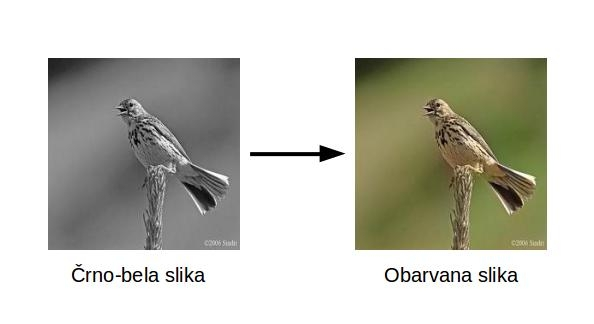
\includegraphics[width=12cm]{imcompare}
\end{center}
\caption{Pristop za vhod vzame črno-belo (sivinsko) sliko, preko nivojev nevronske mreže določi barvne komponente in na izhodu vrne obarvano sliko.}
\label{im:compare}
\end{figure}

Ta problem rešujejo algoritmi za barvanje črno-belih slik. Ti dobijo kot vhod črno-belo sliko, ki ji dodajo barvo, kot je prikazano na sliki \ref{im:compare}. Pristopi za barvanje črno-belih slik se uporabljajo na več področjih: barvanje starih slik, barvanje črno-belih filmov in v pomoč pri umetnosti. V preteklosti so bili pristopi za barvanje slik pol-avtomatski, danes pa jih zamenjuje pristopi, ki obarvajo sliko popolnoma samostojno. Zadnje raziskujemo tudi v tem magistrskem delu.


Za človeka je barvanje črno-belih slik, ki so prikazane na sliki \ref{im:pari-cb-b}, enostavna naloga. Z vsakdanjim opazovanjem sveta se je človek naučil, da je nebo modro z belimi oblaki, drevesa so zelena in cesta je siva. Za objekte, ki nimajo enolično določene barve ljudje lahko ugibamo kakšne barve naj bi predmet bil. Pri tem opravilu je potrebno veliko razumevanja, saj iz sivinskih slik ni možno direktno razbrati barv, namreč pri nastanku sivinske slike se veliko informacij izgubi (dve od treh dimenzij).

\begin{figure}[hbt]
\begin{center}
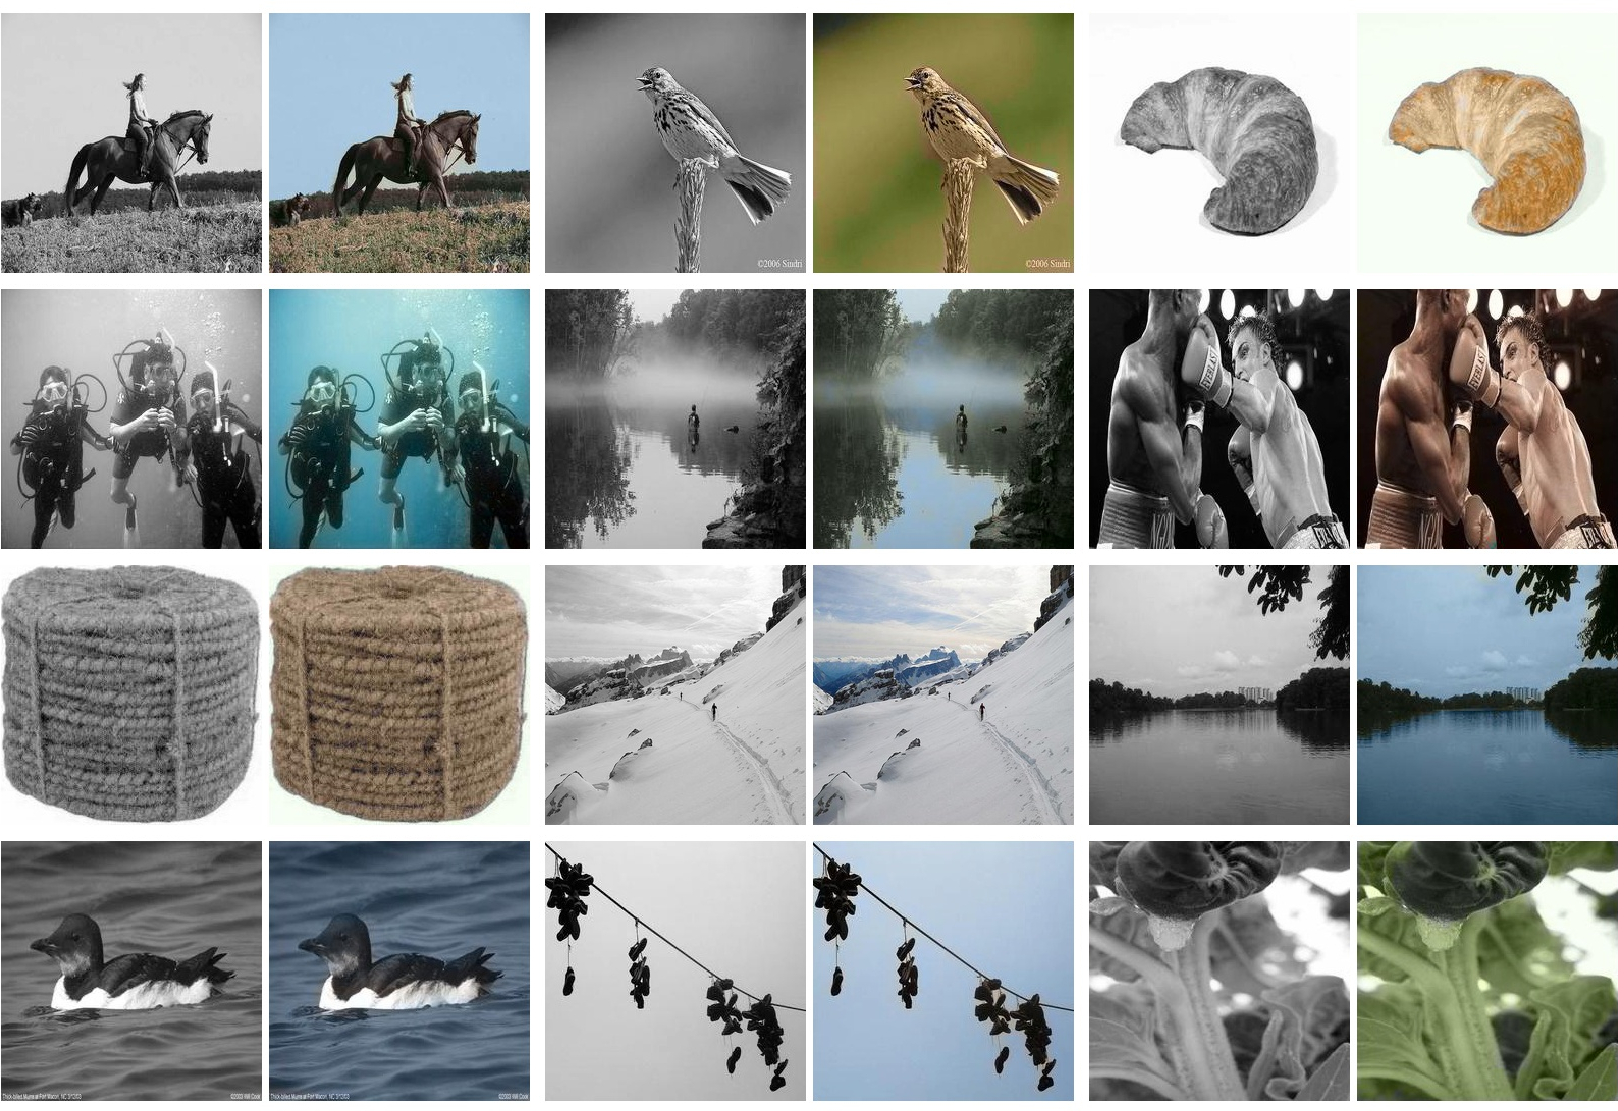
\includegraphics[width=13cm]{black-colored-comparison}
\end{center}
\caption{Primeri barvanja črno-belih slik. Barvanje je bilo izvedeno s pristopi, ki so bili razviti v okviru te magistrske naloge. Za vsako sliko je prikazana črno-bela slika, ki je bila vhod v algoritem in obarvana slika - izhod algoritma. }
\label{im:pari-cb-b}
\end{figure}

Problem postane bolj kompleksen, ko ga želimo rešiti na avtomatski način z računalnikom. Pri tem nam je v pomoč dejstvo, da je možno iz tekstur objektov te prepoznati in jim na ta način določiti njihovo barvo. Pri objektih, ki nimajo enolično določeno barv (na primer avtomobili, stavbe in knjige) je izziv še mnogo težji. Pri tem nam delo olajša dejstvo, da ne želimo, da slika zgleda enaka originalni ampak, da ta zgleda kar se da naravno. Nihče ne bo vedel, da je avtomobil, ki smo ga pobarvali rumeno bil v resnici rdeče barve. 

Za barvanje slik smo izbrali pristope, ki uporabljajo nevronske mreže. Te delujejo podobno, kot človeški možgani. Na začetku jih naučimo tako, da jim podamo čim več primerov barvanja slik. Kasneje nevronska mreža naučeno znanje uporabi, da obarva slike.  
Mreži podamo sivinsko sliko ($L$ kanal barvnega prostora \textit{CIE Lab}), ta pa vrne $a$ in $b$ kanal v istem barvnem prostoru. Za učenje modela potrebujemo veliko količino črno-belih slik z referenčno barvno sliko, kar je praktično zastonj na voljo na spletu. Za treniranje lahko vzamemo katerokoli sliko, jo pretvorimo v barvni prostor \textit{CIE Lab}, kjer $L$ kanal predstavlja sivinsko sliko. 

V tej magistrski nalogi rešujemo problem barvanja črno-belih slik in videov z večimi različnimi pristopi. Za začetek smo implementirali več algoritmov za barvanje črno-belih slik. Rezultate smo med seboj primerjali s računanjem razlike med obarvano in originalno sliko. Rezultate smo primerjali tudi z tremi implementacijami iz sorodnih del. Ker pa obstaja veliko objektov, ki nimajo enolične barve (avtomobili, zgradbe, ...) in naš namen ni doseči enakega barvanja, vendar takega, ki da naravne rezultate, smo barvanje slik ocenjevali s pomočjo uporabnikov. V spletni anketi smo uporabnike spraševali katera slika je bolj naravno obarvana (originalna ali slika obarvana z algoritmom).

Kasneje smo se odločili poskusiti tudi barvanja vida. Za barvanje smo arhitekturo nevronske mreže, ki je najbolje delovala na slikah prilagodili še za video. 

Na začetku si bom v pregledu področja pogledali sorodna dela za barvanje slik, nekaj ozadja o podatkih in globokih nevronskih mrežah. V poglavju \ref{ch:barvanje} so podrobno opisan arhitekture nevronskih mrež in različni pristopi. Opisano je učenje nevronskih mrež, podatki in način evalvacije. V poglavju \ref{ch:rezultati} smo primerjali metode razvite za namen tega magistrskega del z metodami iz sorodnih del, si pogledali kateri pristopi in slike najbolj izstopajo. Pogledali smo si tudi kateri pristop deluje najbolje na slikah večjih velikosti. 



%----------------------------------------------------------------
% Poglavje (Chapter) 2: Pregled področja
%----------------------------------------------------------------
\chapter{Pregled Področja}
\label{ch:pregled}

V tem poglavju si bomo pogledali obstoječe pristope za barvanje črno-belih slik, si pogledali področje globokih nevronskih mrež ter nekaj o predstavitvi slikovnih podatkov in barvnih prostorih.

\section{Obstoječe metode za barvanje črno-belih slik}

Pristope za barvanje črno-belih slik delimo v dve večji skupini. Prva zahteva interakcijo uporabnika in se je več uporabljala predhodno, pri drugi pa barvanje poteka popolnoma avtomatsko.

\subsection{Pristopi, ki zahtevajo interakcijo uporabnika}

To skupion pristopov delimo na tehnike, ki temeljijo na uporabnikovem barvanju manjših delov slik (ang. {\em scribble based}) \cite{levin2004colorization, huang2005adaptive} in tiste, ki temeljijo na primerih (ang. {\em example based}) \cite{Koleini2010, shirley2001color, tai2005local}. Pri prvih uporabnik določi barvo nekaj točk v sliki, te pa algoritem avtomatsko razširi preko cele slike. Kvaliteta barvanja je odvisna od zahtevnosti slike in števila točk, ki jih je uporabnik označil. Pri barvanju na primerih uporabnik izbere referenčno sliko, ki je podobna tisti, ki jo želimo obarvati, algoritem nato lastnosti izbrane slike razširi na drugo sliko ali množico slik. Kvaliteta barvanja je odvisna od tega v kolikšni meri je referenčna slika podobna tisti, ki jo barvamo. Tehnika barvanja s primeri se uporablja za barvanje videov, saj je v tem primeru potrebno ročno pobarvati na primer vsako stoto sliko, na ostale pa algoritem sam razširi lastnosti ročno barvane slike.

\subsection{Popolnoma avtomatski pristopi}

V magistrskem delu se osredotočamo na avtomatske pristope barvanja. To so pristopi, ki samostojno, brez uporabnikovega posredovanja, obarvajo celotno sliko. Prvi dve metodi, ki sta bili predlagani na tem področju, temeljita na značilkah (ang. {\em features}) pridobljenih iz slike. Tukaj gre predvsem za značilke, ki opisujejo intenziteto posamezne barve in značilke, ki opisujejo robove v sliki. Prva metoda uporablja za barvanje nevronsko mrežo \cite{Cheng2015}, ki pa vsebuje zgolj polnopovezane nivoje, druga pa za barvanje uporabi metodo naključnih gozdov (ang. {\em random forest}) \cite{Deshpande2015}. 

Novejši pristopi barvanja črnobelih slik tipično temeljijo na konvolucijskih nevronskih mrežah, ki imajo to lastnost, da v vsakem nivoju same odkrijejo značilke, ki so pomembne za čimboljše barvanje. Prva tovrstna rešitev \cite{Dahl} gradi mrežo na podlagi  že zgrajene šestnajst-nivojske mreže VGG-16, ki so jo razvili na univerzi v Oxfordu \cite{Simonyan2014}. Rešitev uporablja evklidsko cenilno funkcijo in barvni prostor YUV. Slabost te rešitve je, da izhodne barvne slike niso dovolj nasičene in imajo v veliki meri prisotnih več rjavih odtenkov. 

V zadnjem času predlagane rešitve popravijo problem nenasičenosti z uporabo softmax funkcije v zadnjem nivoju nevronske mreže, kar pomeni, da so problem spremenili iz regresijskega v klasifikacijskega.  
Zang in sod. \cite{zhang2016colorful} uporabijo konvolucijsko nevronsko mrežo z več nivoji in aktivacijskimi funkcijami ReLU. Posebnost te mreže je cenilna funkcija. Uporablja križno entropijo, ki pa je v tem primeru izvedena na primerjavi barv posameznih delov slike glede na barvni prostor, ki je kvantiziran. Napake so pomnožene z utežjo, ki določa pogostost barve. Bolj redke barve so obtežene tako, da prispevajo večji delež k napaki, ki jo izračuna cenilna funkcija. S tem so avtorji izboljšali rezultate, tako da se bolj pogosto pojavljajo tudi močnejši odtenki (tisti z višjimi vrednostmi v prostoru \textit{a*b*}, ki so bili prej redkeje zastopani zaradi bolj pogostega pojavljanja nežnejših barv v slikah (barve bližje vrednostim $(0, 0)$ v \textit{a*b*} prostoru.
Pogostost je bila izračunana z analizo vseh slik v podatkovni zbirki Imagenet \cite{ILSVRC15}.  Uporabljajo barvni prostor L*a*b.
 
Larsson in sod. \cite{larsson2016learning} za osnovo uporabijo mrežo VGG-16, iz katere vzamejo tenzorje vsakega nivoja, ki jim povečajo prostorsko dimenzijo, tako da se ujemajo in združijo v enotno matriko. Sledi še en polno-povezan nivo na nivoju točk v sliki. Rezultat klasifikacije je histogram za vsako točko v sliki (histogram z verjetnostmi). Uporabljajo barvni prostor HSV, ki ga prilagodijo zaradi nestabilnosti v eni od točk. Cenilna funkcija, ki jo uporabljajo je KL-divergenca, ki primerja izhodni histogram z v histogram pretvorjeno originalno sliko.
 
Iizuka in sod. \cite{Iizuka2016} uporabijo nevronsko mrežo sestavljeno iz dveh delov. Prvi del poskrbi za napovedovanje vsebine slike, ki se potem združi z glavnim delom in izboljša natančnost barvanja. Uporabili so križno entropijo (ang. {\em cross entropy}) v kombinaciji s cenilno funkcijo \textit{povprečna kvadratna napaka} (ang. {\em Mean squared error}) in barvni prostor L*a*b. Za razliko od prejšnjih dveh metod zadnja ne napoveduje histograma na podlagi kvantiziranega prostora ampak direktno $a*$ in $b*$ vrednost, kar pomeni, da ne uporablja klasifikacije ampak regresijo.

\section{Globoke nevronske mreže}
\label{se:globoke}

Globoke nevronske mreže so algoritmi, ki so zgrajeni na podlagi opazovanja strukture možganov. Uporabljajo se za klasifikacijo, regresijo, gručenje in napovedovalno analizo. Predvsem se uporabljajo na področju slik, kjer je zelo pomembno prepoznavanje objektov in obrazov, razvrščanje slik v skupine glede na podobnost, prepoznavanje gest in barvanje slik \cite{Gibson}.


Nevronska mreža je v osnovi funkcija $f(x)$, ki preslika vhod $x$ v izhod $y$. Med postopkom učenja je ta funkcija optimizirana tako, da najde najboljšo aproksimacijo realnih podatkov \cite{Gibson}. Nevronske mreže so struktura, ki je sestavljena iz več nivojev. Nivoje si lahko predstavljamo kot vrsto vozlišč, ki se odzovejo v primeru da je vzburjenje na njih zadovoljivo - odvisno od aktivacijske funkcije. Struktura vozlišča in nivojev je predstavljena na sliki \ref{im:nn-structure}. Vozlišče pomnoži vsak vhod s trenutnimi vrednostmi uteži doda še bias, vrednosti sešteje in moč aktivacije izračuna s pomočjo tako imenovane aktivacijske funkcije, ki tvori izhod vozlišča. Aktivacijski funkciji rečemo tudi neliearnot, saj poskrbi za to, da nevronska mreža ni le linearna funkcija \cite{Karpathy2016a}. Uteži se skozi postopek učenja spreminjajo in s tem določijo aktivacijo vozlišča. 

\begin{figure}[htb]
\begin{center}
\centering
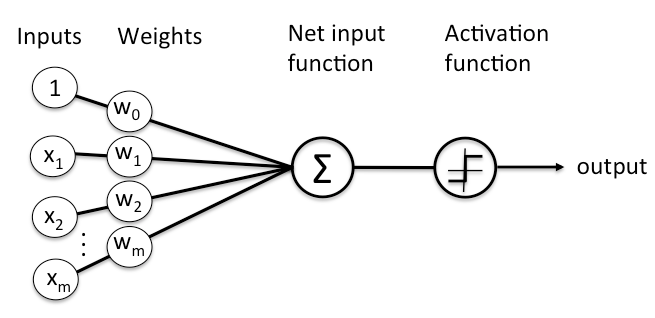
\includegraphics[width=7cm]{node_structure}
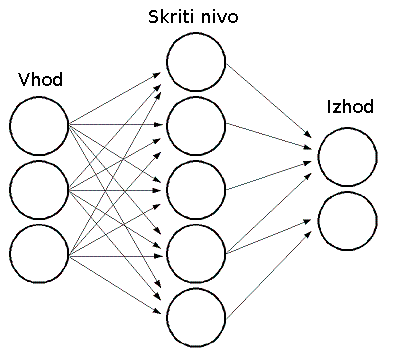
\includegraphics[width=4cm]{nn_structure}
\end{center}
\caption{Leva slika prikazuje zgradbo enega vozlišča, ki ima zasnovo podobno nevronom v možganih. Vhod je lahko izhod prejšnjega nivoja ali vhodni podatki v mrežo, ki se potem pomnožijo z utežmi in seštejejo. Aktivacija poskrbi, da se vozlišče odzove, ko je vzburjenje dovolj veliko. Desna slika prikazuje zgradbo več nivojske nevronske mreže, ki ima vhodni nivo en skriti nivo in izhodni nivo. Iz: Introduction to Deep Neural Networks url{https://deeplearning4j.org/neuralnet-overview} in Neural Networks, url{http://docs.opencv.org/2.4/modules/ml/doc/neural\_networks.html} (dostopano: 21. junij 2017).}
\label{im:nn-structure}
\end{figure}

Nivojem v nevronskih mrežah, ki se nahajajo med vhodnim in izhodnim nivojem rečemo \textit{skriti nivoji} (angl. \textit{hidden layers}) \cite{Karpathy2016a}. Tradicionalni algoritmi na področju strojnega učenja so sestavljeni iz vhodnega, izhodnega nivoja in enega skritega nivoja, \textit{globoka nevronska mreža} (ang. {\em deep neural network}) pa ima vsaj dva skrita nivoja \cite{collobert2008unified}, večinoma pa mnogo več. Vsak nivo globoke nevronske mreže prepozna določen lastnosti vhodnih podatkov. Nivoji, ki se nahajajo globje lahko prepoznajo bolj kompleksne lastnosti podatkov, saj na vhodu, dobijo lastnosti oziroma aktivacije nivoja pred njim. 

Da nevronska mreža daje zadovoljive rezultate je potrebno utežem določiti prave vrednosti. To naredimo s postopkom učenja. Vsaka nevronska mreža ima cenilno funkcijo (ang. loss function), ki pove kako dobre rezultate na testnih podatkih nevronska mreža daje trenutno. V postopku učenja zmanjšujemo vrednost cenilne funkcije z enim od algoritmov optimizacije. 

\subsection{Konvolucijske nevronske mreže}

Ker bi bilo na primeru slik pri uporabi klasičnih nevronskih mrež hitro preveč parametrov, kar bi poleg podaljšanja časa učenja povzročilo tudi prekomerno prilagajanje (ang. overfitting) in pomanjkanje pomnilnika, uporabljamo za take primere konvolucijske nevronske mreže. Te so zelo podobne običajnim nevronskim mrežam. Sestavljene so iz nevronov, ki imajo svoje uteži in bias, ki so učljivi. Operacije znotraj nevrona so podobne tistim pri običajnih nevronskih mrežah, le da so prilagojene pričakovanim vhodnim podatkom - slikam. Vhod v vsak nivo nevronske mreže je torej tenzor z obliko $\check{s}irina \times vi\check{s}ina \times globina$ \cite{Karpathy2016}. Konvolucijske nevronske mreže so v osnovi sestavljene iz treh vrst nivojev:

\begin{itemize}

\item \textbf{Konvolucijski nivo} je glavni gradnik konvolucijske nevronske mreže. Parametri tega nivoja so sestavljeni iz majhnih konvolucijskih jeder, ki pokrivajo majhno polje v širino in višino obenem pa pokrivajo celotni nivo v globino. Med prehodom po nevronski mreži izvedemo konvolucijo po celotni višini in širi vhodnega tenzorja, po globini pa se te izhode teh konvolucij sešteje enako kot pri običajni nevronski mreži. Izhod konvolucije z enim setom jeder je dvodimenzionalna matrika. \cite{lecun1995convolutional} 

\item \textbf{Pooling nivo} je namenjen pod-vzorčenju (ang. downsampling) na določenem nivoju. S tem zmanjšamo število parametrov, kar vpliva zmanjšanje računske zahtevnosti in prekomernega prilagajanja. Deluje na principu, da je točna lokacija značilke manj pomembna kot približna lokacija glede na ostale značilke. \cite{Krizhevsky2012} 

\item \textbf{Polno povezni nivo} je nivo enak skritim nivojem pri klasični nevronski mreži. Večinoma se uporabi se za zadnjih nekaj nivojev pri konvolucijski nevronski mreži, če je to primerno za dano nalogo.

\end{itemize}

\section{Predstavitev slikovnih podatkov in barvni prostori}
\label{se:podatki}

Slike, ki jih uporabljamo za učenje so shranjene v \textit{RGB} \cite{Pm2013} barvnem prostoru. Kot je pokazano v \cite{Iizuka2016} se izkaže, da prostor RGB ni direktno primeren za učenje algoritmov za barvanje iz dveh razlogov:

\begin{itemize}

\item \textbf{Sistem se ne ujema dobro s človeško percepcijo barv}, saj so razdalje med enako sorodnimi barvami različne glede na odtenek \cite{Prangnell}. Na primer, če imamo dva para barv: rdečo in svetlo rdečo, ter modro in svetlo modro, pri čemer sta barvi v vsakem paru za človekov vizualni sistem enako različni, sta razdalji v RGB barvnem prostoru različni . 

\item \textbf{Nima ločenega kanala za svetlost} \cite{Pm2013}. Glede na to, da modeli za barvanje napovedujejo le barvne elemente v sliki, svetlost pa se vzame iz originalne slike, je najbolj priročno, če uporabljamo barvni prostor, ki ima ločen kanal za svetlost, saj je izhod metode kar združena komponenta za svetlost z barvnimi komponentami.

\end{itemize}

\subsection{Izbira primernega barvnega prostora}

Na podlagi teh predpostavk je izbira prostorov omejena na \textit{Lab} \cite{Bansal}, \textit{YUV} \cite{Jack2005} in \textit{HSL} \cite{Pm2013}. Vsi ustrezajo drugi predpostavki iz \ref{se:podatki}. Edini, ki zares ustreza prvi predpostavki je \textit{Lab}. Iz ugotovitev iz sorodnih del \cite{Iizuka2016, Zhang2016, Larsson2016} se tudi najbolje izkaže prostor \textit{CIE L*a*b}.

Obstaja več implementacij barvnega prostora \textit{Lab}, ki vse težijo k dobri aproksimaciji človeškega zaznavnega sistema.  Trenutno se najbolj uporablja \textit{CIE L*a*b*}, ki naj bi bil najboljša aproksimacija človeškega vizualnega sistema \cite{Prangnell}. Prostor ima tudi to prednost, da je neodvisen od naprave. 
Prostor \textit{CIE L*a*b*} predstavi vse barve, ki jih je možno zaznati z tremi barvnimi kanali. $L*$ predstavlja svetlost, $a*$ se razširja od zelene proti rdeči barvi in $b*$ od modre proti rumeni. Prostor je grafično prikazan na sliki \ref{img:lab} $L*$ ser razteza od 0, ki predstavlja črno barvo, do 100, ki predstavlja belo barvo \cite{Weatherall1992}. $a*$ in $b*$ komponenti nimata uradne omejitve, vendar sta v implementacijah ponavadi omejene na vrednosti v intervalu $[-128, 127]$, kar je možno predstaviti z 8 bitnim celim številom \cite{Everding}. Ker zaradi pretvorb iz barvnega prostora \textit{RGB} vrednosti višje od $100$ ali nižje $-100$ redko dosežemo smo opazili, da nekatere implementacije omejijo barvne komponente na interval $[-100, 100]$. Za pomoč pri implementaciji nevronske mreže smo sami preizkusili kakšen je dejanski interval barv pretvorjenih iz \textit{RGB} barvnega prostora. Intervale si lahko pogledate v tabeli \ref{tab:rgbcie}.

\begin{figure}[hbt]
\begin{center}
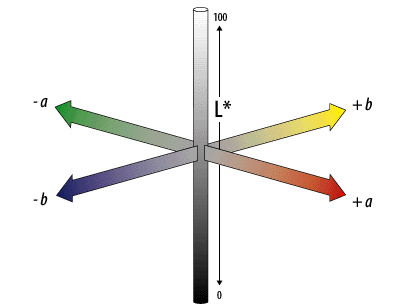
\includegraphics[width=6cm]{cielab}

\end{center}
\caption{Slika prikazuje kanale barvnega prostora CIE L*a*b*. L* predstavlja svetlost, a* se razteza od zelene barve v najbolj negativni točki proti rdeči barvi, b* ser razteza od modre proti rumeni. Nasprotujoče barve na kanalih a* in b* se nikoli ne kombinirajo v odtenek. Iz: Adobe, Technical Guid, CIELAB, \url{http://dba.med.sc.edu/price/irf/Adobe_tg/models/cielab.html} (dostopano: 24. junij 2017)}
\label{nn-structure}
\end{figure}

\begin{table}
\caption{Njavečje in njmanjše vrednosti posamezne komponente CIE L*a*b* barvnega prostora, pri pretvorbi  barv iz barvnega prostora RGB. Pretvorba je bila narejena z uporabo osvetlitve $D65$, ki določa temperaturo bele točke. Izkaže se, da je večina vrednosti komponent $a*b*$ znotraj intervala $[-100, 100]$. }
\begin{center}
    \begin{tabular}{l|ccc}
        Kanal & Najmanjša vrednost & Največja vrednost \\
        \hline
        L* & 0 & 100 \\
        a* & -86.185 & 98,254 \\
        b* & -107.863 & 94.482 \\
    \end{tabular}
\end{center}
\label{tab:rgbcie}
\end{table}

\subsection{Pretvarjanje med RGB in CIE L*a*b* barvnim prostorom}

Za pretvorbo med prostoroma ni enostavne enačbe, saj je \textit{RGB} barvni prostor odvisen od naprav, \textit{CIE L*a*b*} pa je neodvisen. Tako se pretvorba zgodi v treh korakih \cite{Connolly1997}: 

\begin{enumerate}

\item \textbf{Pretvorba iz RGB v sRGB ali Adobe RGB}, saj sta ta barvna prostora neodvisna od naprave. Ta pretvorba je odvisna od naprave. Slike, ki jih bomo uporabili v našem delu so že v \textit{sRGB} obliki, saj so bile pretvorjene, ko so bile zajete z fotoaparatom.

\item \textbf{Pretvorba v CIE 1931 barvni prostor} ali drugače imenovan \textit{CIE XYZ} barni prostor. Ta pretvorba se izvede s pomočjo linearne pretvorbe z matriko. Matrika je odvisna od izibire referenčne bele barve. Običajno se izbere referenčno temperaturo belo točke \textit{D65}, ki je tudi standardizirana\footnotemark \cite{Ohta2005}.

\footnotetext{Zapis na uradni strani komisije International Commision on Illumination (krajše CIE), ki je postavila standard pravi, da se kot standardno uporablja referenčno temperaturo bele točke D65: \url{http://cie.co.at/index.php?i_ca_id=484}}

\item \textbf{Pretvorba iz CIE XYZ v L*a*b*} se izvede po enačbah opisanih v \cite{Schwiegerling2004}.  % če je potrebno jih lahko prepišem

\end{enumerate}




%----------------------------------------------------------------
% Poglavje (Chapter) 3: Pregled področja
%----------------------------------------------------------------

\chapter{Barvanje črno-belih slik z globokimi nevronskimi mrežami}
\label{ch:barvanje}

V tem poglavju predstavljamo arhitekture nevronskih mrež, ki smo jih načrtovali, pogledali si bom pristope z regresijo in klasifikacijo in predstavili učenje. Opisan je eksperiment z barvanjem večjih slik od tistih na katerih je bila mreža naučena, predstavljeni so učni in testni podatki ter način evalvacije. 

\section{Arhitekture}
\label{ch:arhitekture}

V grobem smo v okviru magistrske naloge implementirali štiri arhitekture nevronskih mrež, kasneje smo te arhitekture kombinirali z različnimi cenilnimi funkcijami, pristopi (regresijski ali klasifikacijski) in načini napovedovanja (napovedovanje po delih ali na celi sliki).

\subsection{Plitva arhitektura z globalno mrežo}
\label{ch:plitva}

Plitva arhitektura z globalno mrežo je sestavljena iz dveh delov, ki se kasneje združita v enotno mrežo. Glavni del predstavlja zaporedje konvolucijskih nivojev, ki na vhodu vzamejo sivinsko sliko, izhod pa je obarvana slika. Po osmih kovolucijskih nivojih se mreža združi z tako imenovano globalno mrežo, ki napoveduje objekt, ki ga slika predstavlja. Za globalno mrežo smo vzeli že naučeno mrežo VGG-16 \cite{Simonyan2014}, ki smo ji odvzeli zadnji polno-povezani nivo in ji dodali nov polno-povezani nivo z izhodnim tenzorjem dolžine 256. Ker je ta mreža namenjena sprejemu barvnih RGB slik smo vhod prilagodili tako, da sprejme sivinsko sliko na vseh treh kanalih. Arhitektura nevronske mreže je predstavljena na sliki \ref{im:arh1} in v tabeli \ref{tab:arh1} v prilogi.

Na tem mestu bi bilo smiselno opisati še kako poteka združevanje glavne in globalne mreže. Vhod v element za združevanje sta tenzorja velikosti $w/8 x h/8 x 256$ iz glavne mreže in enodimenzionalni tenzor velikosti $256$ iz globalne mreže. Pri tem $w$ in $h$ predstavljata širino in višino vhodne slike v mrežo. Pri združevanju vsakemu elementu širine in višine prvega tenzorja pridružimo tenzor globalne mreže, kot prikazuje slika \ref{im:fusion}. Tako na izhodu dobimo tenzor velikosti $\frac{w}{8} \times \frac{h}{8} \times 512$. 
 
\begin{figure}[hbt]
\begin{center}
\centering
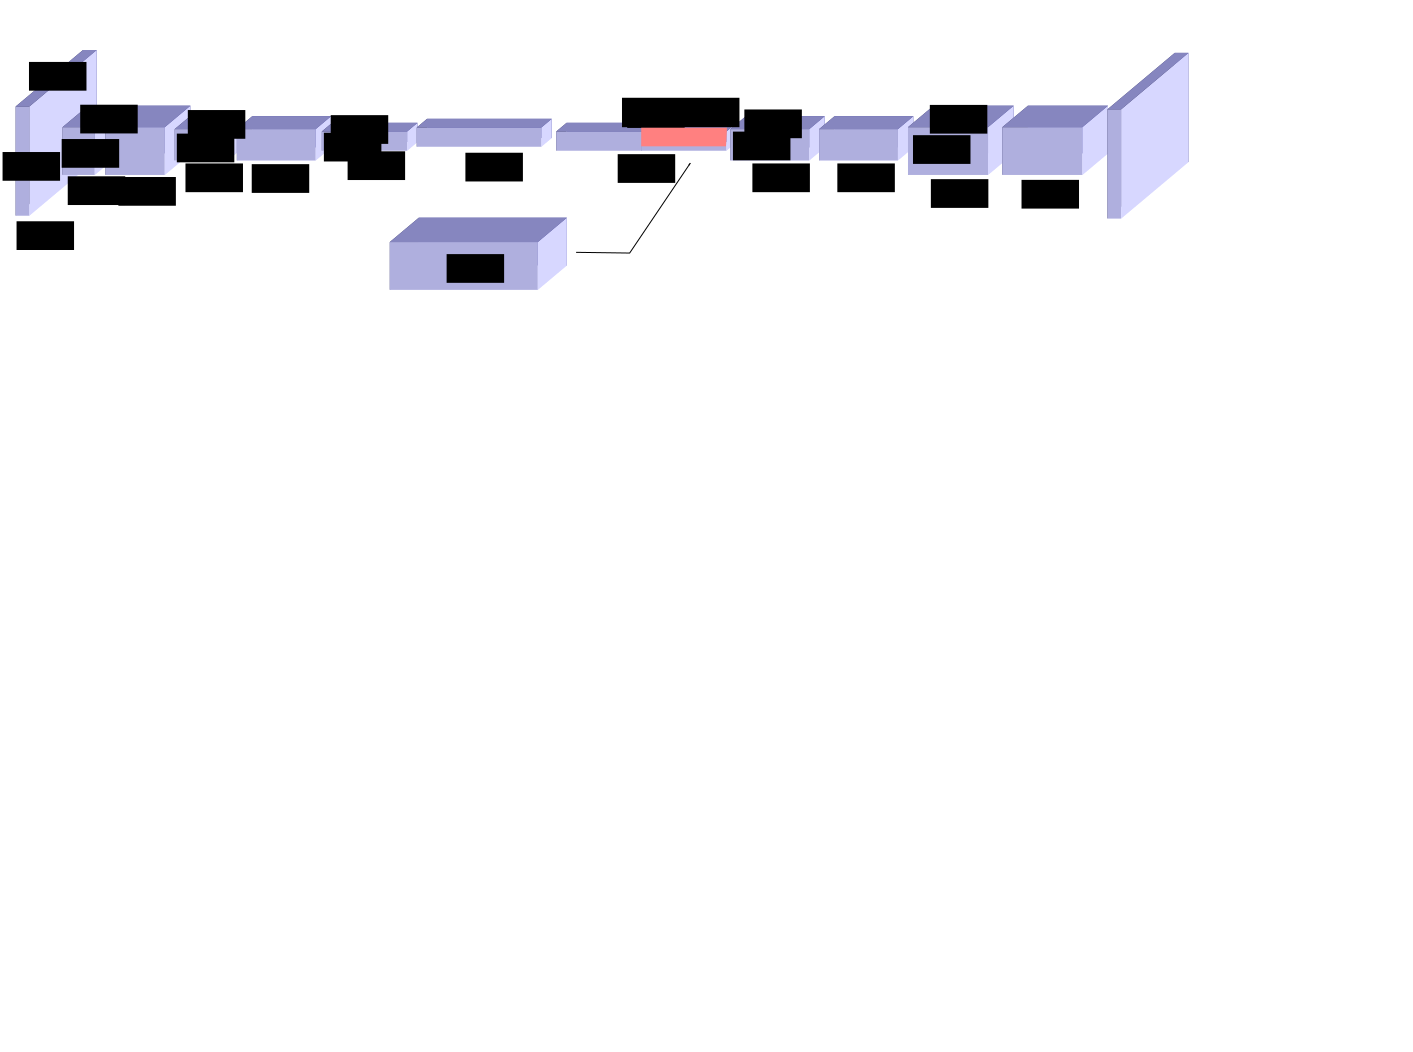
\includegraphics[width=13cm]{arh1}
\end{center}
\caption{Slika prikazuje velikosti tenzorjev skozi plitvo arhitekturo z globalno nevronsko mrežo. $w$ in $h$ predstavljata širino in višino vhodne slike. Podrobnosti nivoja združitev so predstavljene na sliki \ref{im:fusion}, nivo izhodne slike ni natančneje označen, saj se razlikuje v različnih implementacijah, ki so podrobneje opisane v poglavjih \ref{ch:regression-methods} in \ref{ch:classification-methods}. }
\label{im:arh1}
\end{figure}

\begin{figure}[hbt]
\begin{center}
\centering
\includegraphics[width=8cm]{fusion}
\end{center}
\caption{Prikaz delovanje nivoja združevanja glavne nevronske mreže z globalno nevronsko mrežo. K izhodu glavne nevronske mreže (modri tenzor) dodamo tenzor iz globalne mreže (rdeči tenzor), tako da ga priključimo k vsem prostorskim lokacija kot dodatnih 256 kanalov. Izhodni tenzor ima tako za izhod 512 kanalov.}
\label{im:fusion}
\end{figure}

% l2 regularizacija citation \cite{mackay1992practical}

\subsection{Globja arhitektura z globalno mrežo}
\label{ch:globjaz}

Ta arhitektura ima v osnovi enako zasnovo, kot arhitektura v poglavju \ref{ch:plitva}. Razlika se pojavi pri globini glavne mreže. Ta ima namreč 14 konvolucijskih nivojev pred združitvijo in 7 po združitvi kot lahko vidite na sliki \ref{im:arh2} in tabeli \ref{tab:arh2} v prilogi. Za razliko od arhitekture opisane v poglavju \ref{ch:plitva} ta za zmanjševanje prostorskih (ang. {\em spatial}) dimenzij uporablja \textit{maksimalno združevanje} (ang. {\em max pooling}) \cite{Krizhevsky2012} in za povečevanje le teh v zadnjih nivojih uporablja \textit{transponirano konvolucijo} (ang. {\em transpose convolution}) \cite{Dumoulin2016} imenovano tudi dekonvlucija. Združevanja glavne in globalne mreže se izvede na način opisan v poglavju \ref{ch:plitva}.

Ta arhitektura prinaša še eno spremembo. To so tako imenovane rezidualne povezave, ki so bile prvič uporabljene v nevronski mreži ResNet zasnovani s strani Microsoft Research \cite{Wu2017}, ki je leta 2015 zmagala na tekmovanju ImageNet \cite{ILSVRC15}. Te povezave so na sliki \ref{im:arh2} označene s puščicami nad nevronsko mrežo in predstavljajo povezavo, ki na mestu kamor kaže puščica, združi trenutni tenzor z tenzorjem izračunanim pred dvema nivojema. Operacija združevanja je seštevanje isto ležečih elementov v tenzorju.  

\begin{figure}[hbt]
\begin{center}
\centering
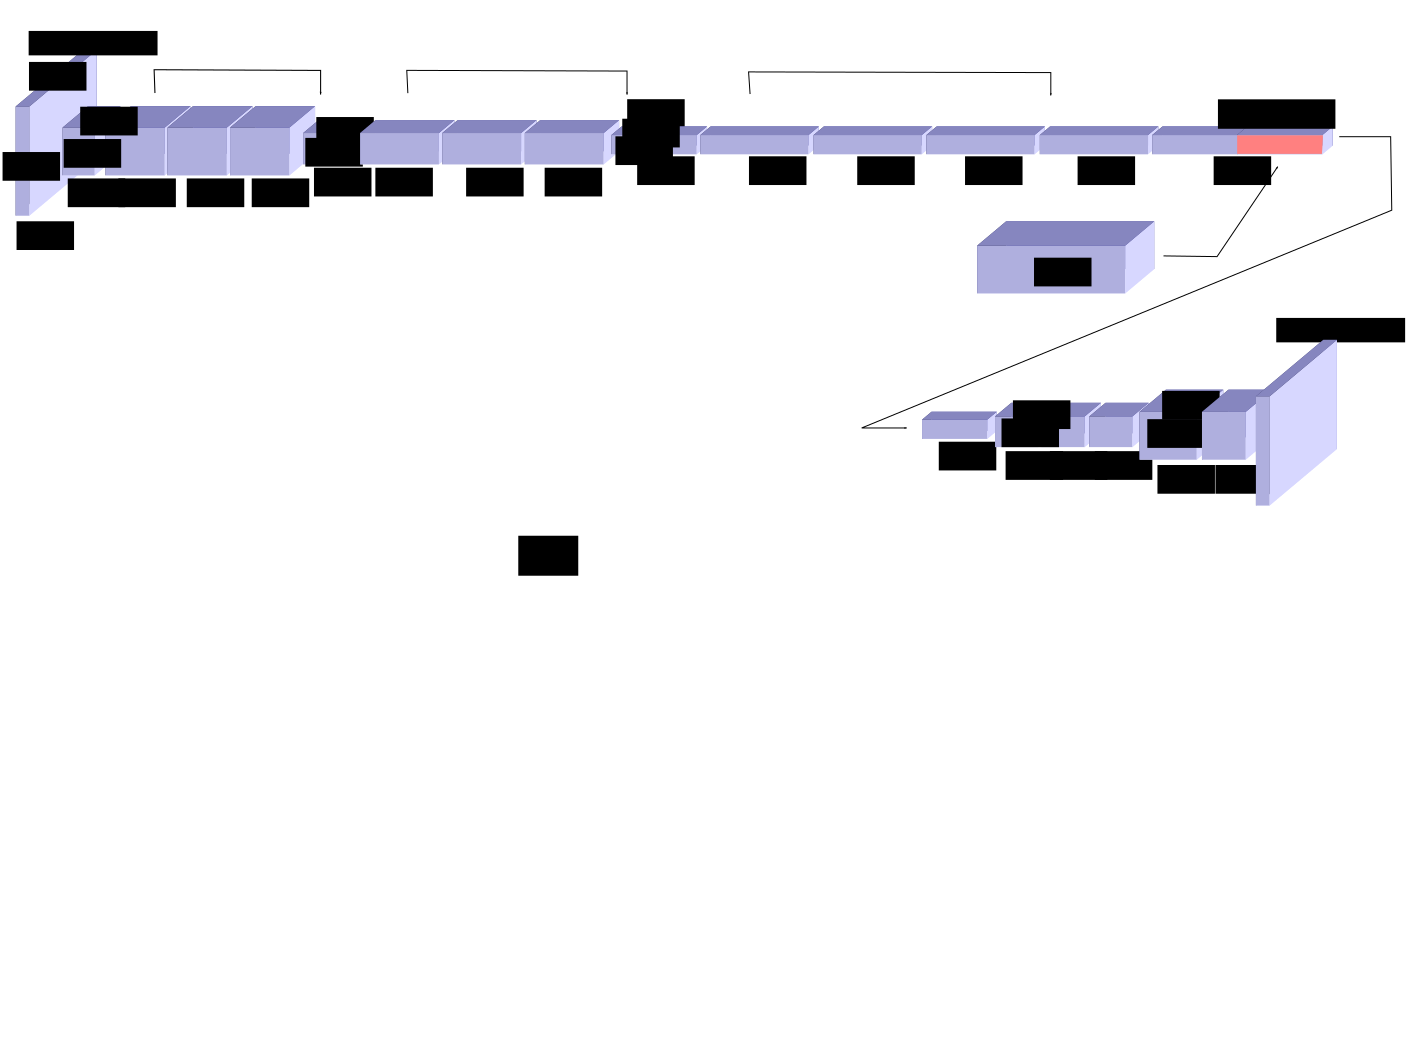
\includegraphics[width=13cm]{arh2}
\end{center}
\caption{Slika prikazuje velikosti tenzorjev skozi globjo arhitekturo z globalno nevronsko mrežo. $w$ in $h$ predstavljata širino in višino vhodne slike. Podrobnosti nivoja združitev so predstavljene na sliki \ref{im:fusion}, nivo izhodne slike ni natančneje označen, saj se razlikuje v različnih implementacijah, ki so podrobneje opisane v v poglavjih \ref{ch:regression-methods} in \ref{ch:classification-methods}. }
\label{im:arh2}
\end{figure}

\subsection{Globja arhitektura brez globalne mreže}

Ta arhitektura je enaka tisti opisani v poglavju \label{globjaz} in prikazani na sliki \ref{im:arh2} v glavnem delu in se razlikuje po tem, da nima globalne mreže. Torej nima mreže, ki se pridruži v nivoju združitve, zaradi tega smo tudi ta nivo izpustili. Mreža za vhod vzame črno-belo sliko z enim kanalom in izračuna barvno sliko na izhodu. Ta arhitektura je bila načrtovana z namenom, da se preveri če ima globalna mreža prisotna v arhitekturah predstavljenih v poglavjih \ref{ch:globjaz} in \ref{ch:plitva} kakšen vpliv na rezultate.

\subsection{Dopolnjena VGG-16 arhitektura}

Arhitektura je zgrajena tako, da za vrh mreže uporabimo mrežo VGG-16 \cite{Simonyan2014}, kateri smo odstranili vse polno povezane nivoje. Arhitektura je narejena tako, da na vhodu sprejme črno-belo sliko, ki jo potem prilagodimo za vhod mreže VGG-16, tako da ima tri vhodne kanale. Te dobimo tako, da vzamemo sivinsko sliko za vsak vhodni kanal. Tenzor, ki ga vrne zadnji konvolucijski nivo mreže VGG-16 podamo na vhod lastne mreže, ki je prikazana na sliki \ref{im:arh4} in podrobno opisana v tabeli \ref{tab:arh4} v prilogi. Lastna mreža ima še 8 konvolucijskih nivojev in 4 nivoje nad-vzorčenja, ki poskrbijo za povečanje dimenzije prostorskih komponent. Po zadnjem nivoju izvedemo še povečanje slike za faktor 2, saj se nad-vzorčenje izkaže kot slabša možnost.

\begin{figure}
\begin{center}
\centering
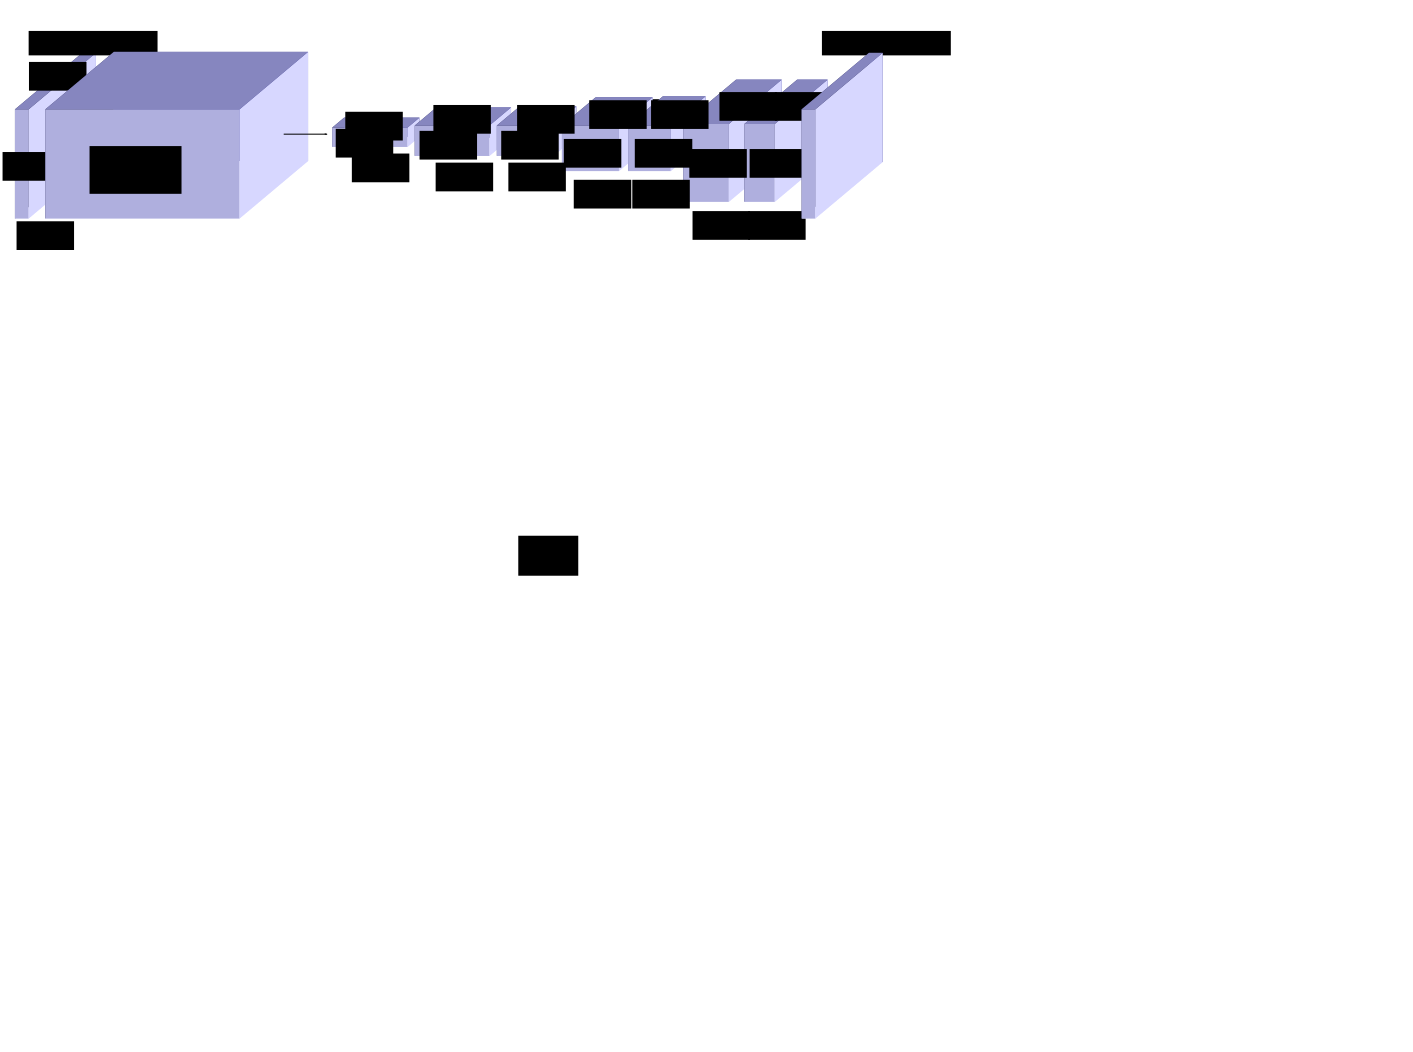
\includegraphics[width=12cm]{arh4}
\end{center}
\caption{Slika prikazuje velikosti tenzorjev skozi dopolnjeno VGG-16 arhitekturo. $w$ in $h$ predstavljata širino in višino vhodne slike. Nivo izhodne slike ni natančneje označen, saj se razlikuje v različnih implementacijah, ki so podrobneje opisane v poglavjih \ref{ch:regression-methods} in \ref{ch:classification-methods}. Prvi večji blok predstavlja mrežo VGG-16 \cite{Simonyan2014}}
\label{im:arh4}
\end{figure}

\section{Pristopi z regresijo}
\label{ch:regression-methods}

V tem poglavju bomo prestavili regresijske metode, ki smo jih uporabili. Te se imenujejo tako, saj pri napovedovanju barve direktno napovejo vrednosti $a*$ in $b*$ barvne komponente v prostoru \textit{CIE L*a*b*}. Tu mreža predstavlja regresijsko funkcijo $y = f(x)$ za vsako točko na slike, ki na vhod dobi točko sivinske slike $x$, izhod pa je kar vrednost $y$, ki predstavlja določeno barvo v našem primeru sta to dve vrednosti $a*$ in $b*$.

Na sliki \ref{im:reg-scheme} je prikazan postopek delovanja, ki je skupen vsem regresijskim metodam opisanim v nadaljevanju. Da dobimo barvno sliko moramo izhod iz mreže, ki predstavlja barvne komponente združiti s sivinsko.


\begin{figure}[hbt]
\begin{center}
\centering
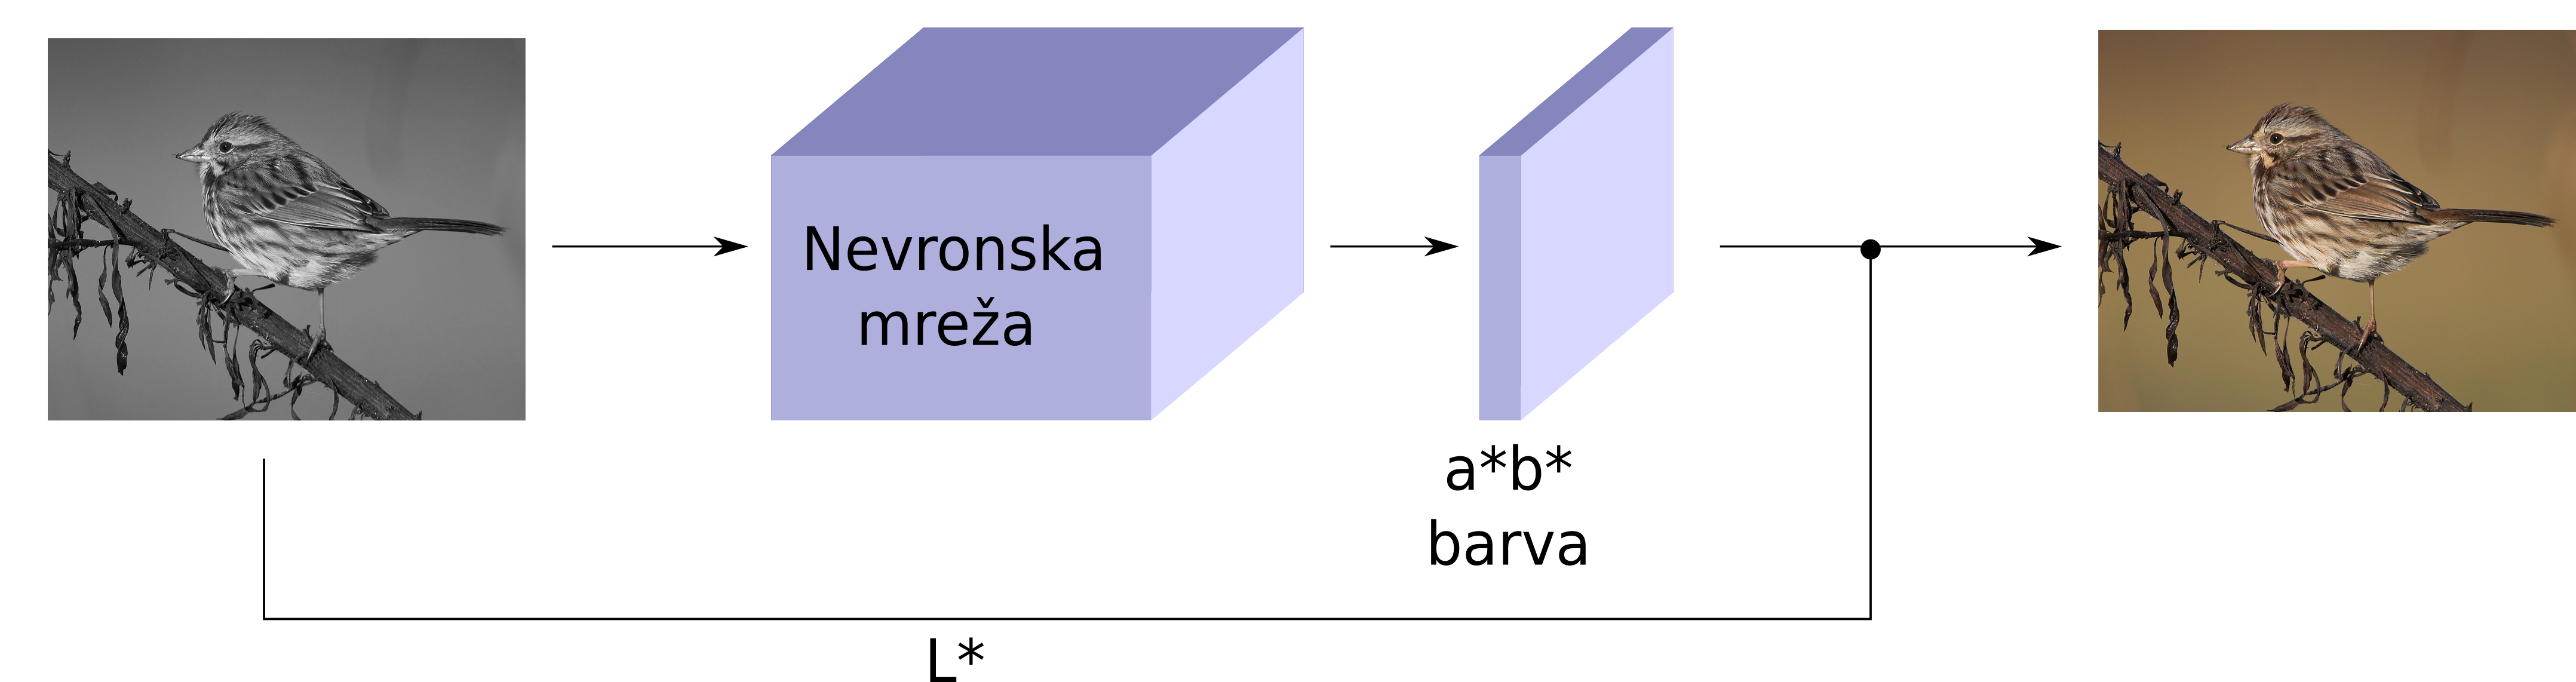
\includegraphics[width=12cm]{regresija-shema}
\end{center}
\caption{Shematski prikaz delovanja regresijske metode, ki na vhod prejme črno-belo sliko, s pomočjo nevronske mreže izračuna barvni komponenti $a*$ in $b*$ barvnega prostora \textit{CIE L*a*b*} ter to združi s sivinsko sliko $L*$, da dobi obarvano sliko. }
\label{im:reg-scheme}
\end{figure}

\subsection{Pristopi na delih slik}
\label{ch:parts-im}

V to skupino lahko uvrstimo tri metode, ki imajo skupno to, da smo barvanje izvajali na majhnih delih slik. Ta princip smo razvili z opazovanjem delovanja človeškega zaznavnega sistema, ki se bi lotil barvanja po delih, na sliki bi zaznal objekte ločeno barval. Na primer najprej vodo, nato gozd in kasneje še nebo. 

Sliko smo preden smo jo podali nevronski mreži razdelili na koščke velikosti $32 \times 32$. Pri tem sta se sosednja koščka prekrivala za $16$ slikovnih točk kot je prikazano na sliki \ref{im:overlapping}. 
V arhitekturah, kjer je bila prisotna ločena globalna mreža, je ta še vedno na vhodu prejela celotno sliko, s katero smo pridobili globalni koncept slike. Dele slik smo kasneje sestavili z metodo prekrivanja, tako da so imele vrednosti točk pri robu manjši vpliv kot tiste pri sredini. Vpliv barvne točke se je izračunal po enačbi \ref{eq:1}, kjer $x$ predstavlja vrednost slikovne točke, $d$ predstavlja oddaljenost od središča v številu slikovnih točk. Enačba se ločeno uporablja v vertikalni in horizontalni smeri. 

\begin{equation}
y = \frac{d}{16} * x
\label{eq:1}
\end{equation}

\begin{figure}[hbt]
\begin{center}
\centering
\includegraphics[width=8.5cm]{overlapping}
\end{center}
\caption{Shema prikazuje razdeljevaje slike velikosti $128 \times 128$ slikovnih točk, ki jo v vsaki smeri razdelimo na $7$ enakih delov velikosti $32$. Rdeč in zelen kvadrat prikazujeta prva dva dela s konceptom prekrivanja. Enak sistem uporabimo v vertikalni smeri.}
\label{im:overlapping}
\end{figure}

Z takim načinom dela pričakujemo pohitritev učenja, saj menimo, da je že del slike dovolj da se mreža nauči celotne teksture objekta. Na primer, da se naučimo barvati vodo ne potrebujemo celotnega območja vode na sliki, ki včasih lahko prekriva tudi pol ali več slike, ampak le en del. Z učenjem mreže na manjših vhodnih tenzorjih, kar dosežemo z učenjem po delih, se čas, ki ga mreža porabi za učenje ene serije (ang. {\em batcha}) podatkov zmanjša. 

V tabeli \ref{tab:methods-parts} so predstavljene podrobnosti vsake od metod barvanja po delih.

\begin{table}[hbt]
\caption{Regresijski pristopi po delih, njihove arhitekture, ki so podrobneje opisane v poglavju \ref{ch:arhitekture} in cenilne funkcije uporabljene za učenje. $MSE$ je povprečna kvadratna napaka (ang. {\em mean squared error}).}
\begin{center}
    \begin{tabular}{l|cc}
	Ime metode & Arhitektura & Cenilna funkcija \\
	\hline
	Reg. po delih & Globja arh. z glob. mr. & MSE \\
	\hspace{0.5em} - brez softmax & Globja arh. z glob. mr. & MSE \\
	\hspace{0.5em} - brez globalne mreže & Globja arh. brez glob. mr. & MSE \\
    \end{tabular}
\end{center}
\label{tab:methods-parts}
\end{table}

\subsection{Pristopi na celih slikah}

Za primerjavo točnosti metod na delih slik s tistimi na celih slikah. Smo dve metodi opisane v poglavju \ref{ch:parts-im} pretvorili v metode za barvanje na celih slikah. Tej smo dodali še eno metodo, saj zaradi večkratnega pomanjšanja prostorskih dimenzij znotraj arhitekture ne more biti realizirana na manjših delih slik.

V tabeli \ref{tab:methods-whole} so podrobno predstavljene lastnosti teh metod. 

\begin{table}[hbt]
\caption{Regresijski pristopi na celih slikah, njihove arhitekture, ki so podrobneje opisane v poglavju \ref{ch:arhitekture} in cenilne funkcije uporabljene za učenje. $MSE$ je povprečna kvadratna napaka (ang. {\em mean squared error}).}
\begin{center}
\begin{tabular}{l|cc}
Ime metode & Arhitektura & Cenilna funkcija \\
\hline
Reg. cela slika & Globja arh. z glob. mr. & MSE \\
\hspace{0.5em} - brez globalne mreže & Globja arh. brez glob. mr. & MSE \\
Reg. cela slika VGG & Dop. VGG-16 arh. & MSE \\
\end{tabular}
\end{center}
\label{tab:methods-whole}
\end{table}

\section{Pristopi s klasifikacijo}
\label{ch:classification-methods}

Razvili smo tudi štiri metode, ki namesto regresije uporabljata klasifikacijo. To so pristopi, kjer direktno ne napovemo številčne vrednosti barve ampak to določimo s pomočjo klasifikacije v enega od razredov, ki predstavljajo nekaj sosednjih odtenkov v sliki. Klasifikacija se izvede z uporabo softmax funkcije v zadnjem nivoju mreže. Izhodi teh mrež so verjetnosti za  vsakega od razredov. Kot je prikazano na sliki \ref{im:class-scheme} se te vrednosti pretvorijo v vrednosti $a*$ in $b*$.

\begin{figure}[hbt]
\begin{center}
\centering
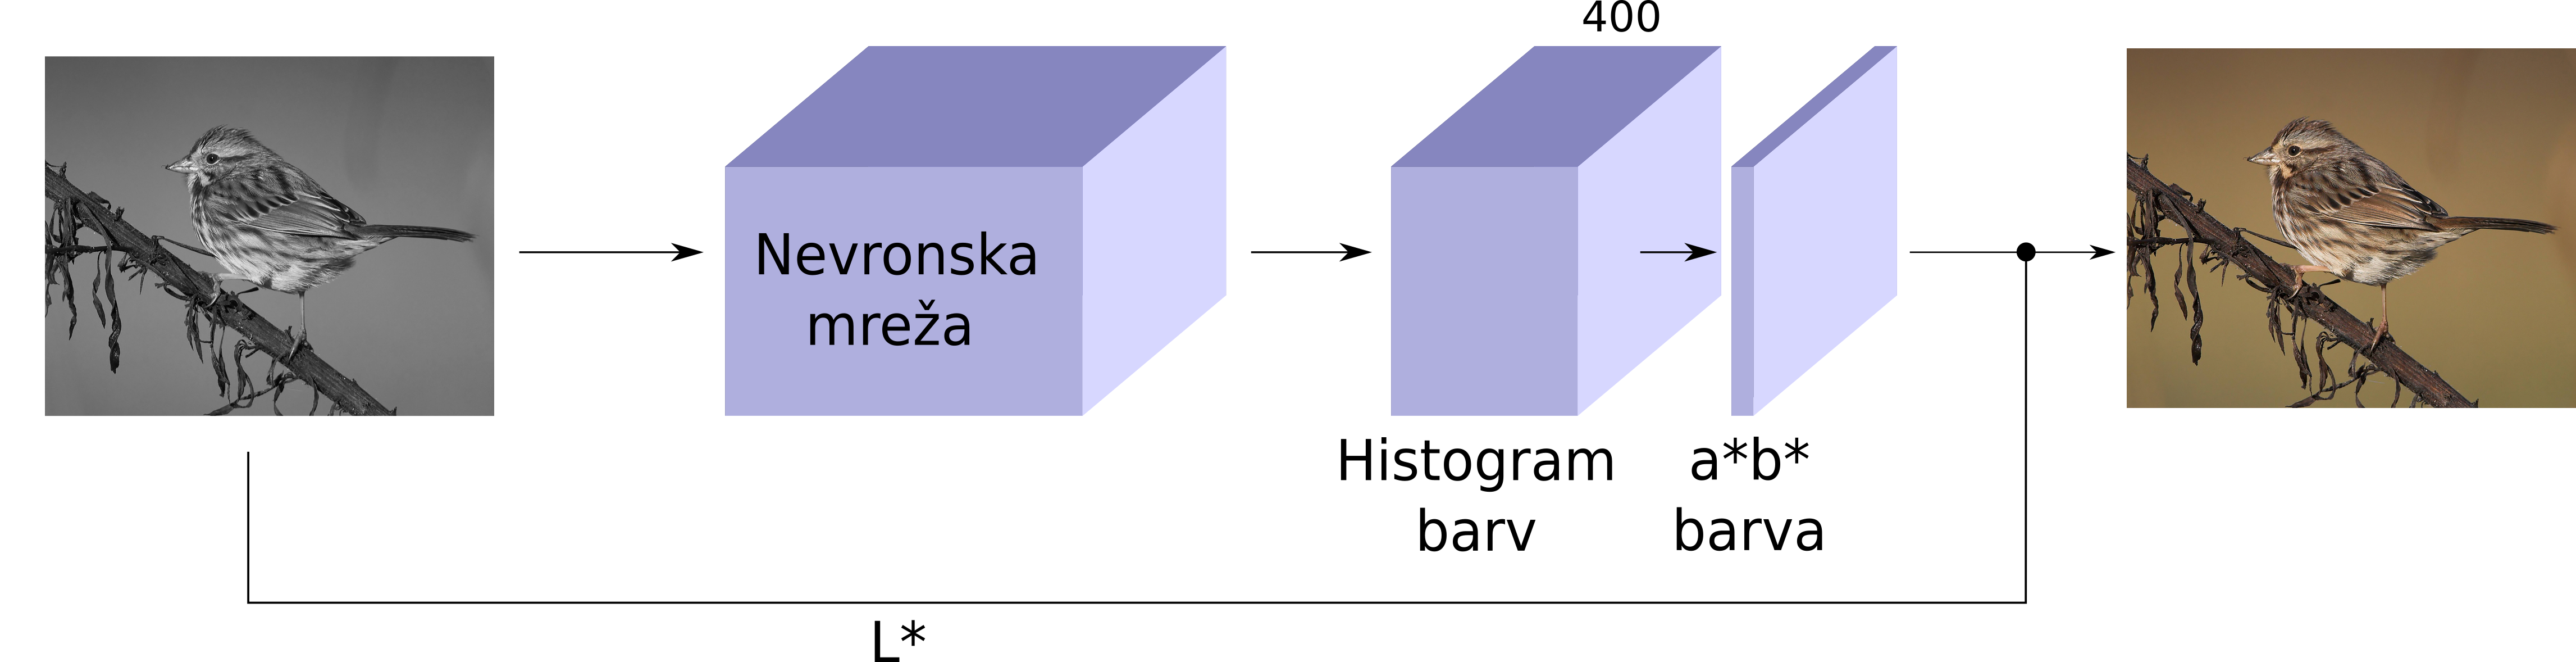
\includegraphics[width=12cm]{classification-scheme}
\end{center}
\caption{}
\label{im:class-scheme}
\end{figure}

Razrede smo dobili tako, da barvni prostor \textit{CIE L*a*b*} razdelimo v 400 razredov po komponentah $a*$ in $b*$. Vsako od komponent smo razdelili v $20$ razredov med vrednostima $-100$ do $100$, kar pomeni da vsak razred zajema interval širine $10$. 

Za delovanje mreže moramo pretvoriti $a*b*$ zapis v histogram in obratno. Pretvorba v iz zapisa $a*b*$ v histogram je potrebna saj moramo pri učenju referenčno sliko (ang. {\em ground truth}) pretvoriti v histogram, da lahko izračunamo napako. To se izvedemo s enačbo \ref{eq:ab2hist}, kjer $a$ in $b$ predstavljata $a*$ ali $b*$ vrednost slikovne točke, $y$ pa indeks razreda v histogramu. 

\begin{equation}
y = 20 \left\lfloor\frac{a + 100}{10} \right\rfloor + \left\lfloor\frac{b + 100}{10} \right\rfloor
\label{eq:ab2hist}
\end{equation}

Pretvorba iz histograma v $a*$ in $b*$ se uporabi pri pretvorbi ocenjenih barvnih vrednosti s pomočjo mreže in se izvede po enačbah \ref{eq:hist2ab}. Pri tem $a$ in $b$ predstavljata $a*$ in $b*$ barvne vrednosti slikovne točke, $y$ predstavlja indeks razreda v histogramu, ki je bil napovedan z največjo verjetnostjo. 

\begin{gather*}
a = 10 \left\lfloor \frac{y}{20} \right\rfloor - 100 + 5 \\
b = 10 (y\mod 20)  - 100 + 5
\label{eq:hist2ab}
\end{gather*}

Pristope s klasifikacijo smo preizkusili, ker so v delih \cite{Larsson2016, Zhang2016} ugotovili, da so rezultati teh metod, slike, ki so bolj nasičene in realnih barv. V tabeli \ref{tab:methods-class}.

\begin{table}[hbt]
\caption{Klasifikacijski pristopi po delih, njihove arhitekture, ki so podrobneje opisane v poglavju \ref{ch:arhitekture} in cenilne funkcije uporabljene za učenje. $KL-divergenca$ je Kullback-leibler divergenca \cite{joyce2011kullback}, $CCE$ predstavlja kategorično križno entropijo \cite{Mannor2005}. }
\begin{center}
    \begin{tabular}{l|cc}
	Ime metode & Arhitektura & Cenilna funkcija \\
	\hline
	Klas. brez uteži - plitva arh. & Plitva arh. z glob. mr. &  KL-divergenca \\
	Klas. brez uteži - globja arh. & Globja arh. z glob. mr. & CCE \\
	Klas. z utežmi - plitva arh. & Plitva arh. z glob. mr. & CCE \\
	Klas. z utežmi - globja arh. & Globja arh. z glob. mr. & CCE \\
    \end{tabular}
\end{center}
\label{tab:methods-class}
\end{table}



\section{Postopek učenja}

V tem poglavju bomo predstavili podrobnosti učenja na manjši množici, na večji učni množici in si za konec še pogledali kakšne značilke prepozna posamezni nivo nevronske mreže. 

\subsection{Učenje na manjši učni množici}

Za učenje na manjši množici smo izbrali vse metode opisane v poglavjih \ref{ch:regression-methods} in \ref{ch:classification-methods}. Za primerjavo natančnosti smo dodatno še implementirali metode razvite s strani R. Dahl-a \cite{Dahl}, Iizuka in sod. \cite{Iizuka2016} in Zhang in sod. \cite{zhang2016colorful}.

Za posodabljanje parametrov smo uporabili Adam optimizator \cite{DBLP:journals/corr/KingmaB14}. Pri tem sta se za dobre izkazali naslednji parametri, ki so prikazani v tabeli \ref{tab:adam-param}. Pri vseh metodah smo uporabili velikost serije (ang. {\em batch size}) $32$, razen pri treniranju metode Zhang in sod., kjer smo morali zaradi večjih dimenzij tenzorjev in posledično pomakanju spomina uporabiti velikost serije $8$.

\begin{table}[hbt]
\caption{Parametri, s katerim smo nastavili Adam optimizatior. }
\begin{center}
\begin{tabular}{l|cc}
Parameter & Vrednost parametra \\
\hline
stopnja učenja (ang. {\em learning rate}) & $10^{-4}$ \\ 
beta 1 & $0.9$ \\
beta 2 & $0.99$ \\ 
epsilon & $10^{-8}$ \\
\end{tabular}
\end{center}
\label{tab:adam-param}
\end{table}

Pri treniranju smo beležili vrednosti cenilne funkcije tako na množici podatkov za treniranje in množici podatkov za validacijo po končanem vsakem prehod čez vse podatke (ang. {\em epoch}. S tem smo opazovali kdaj je določena metoda optimalno naučena. To se v našem primeru zgodi v trenutku, ko vrednost cenilne funkcije na validacijski množici preneha padati ali celo začne naraščati. V tem trenutku je naša mreža optimalno naučena, zato smo te uteži uporabili za testiranje. Grafi padanja cenilnih funkcij za vse pristope so prikazani na sliki \ref{im:histograms-100}. 


\begin{figure}[htb]
\begin{center}
\centering
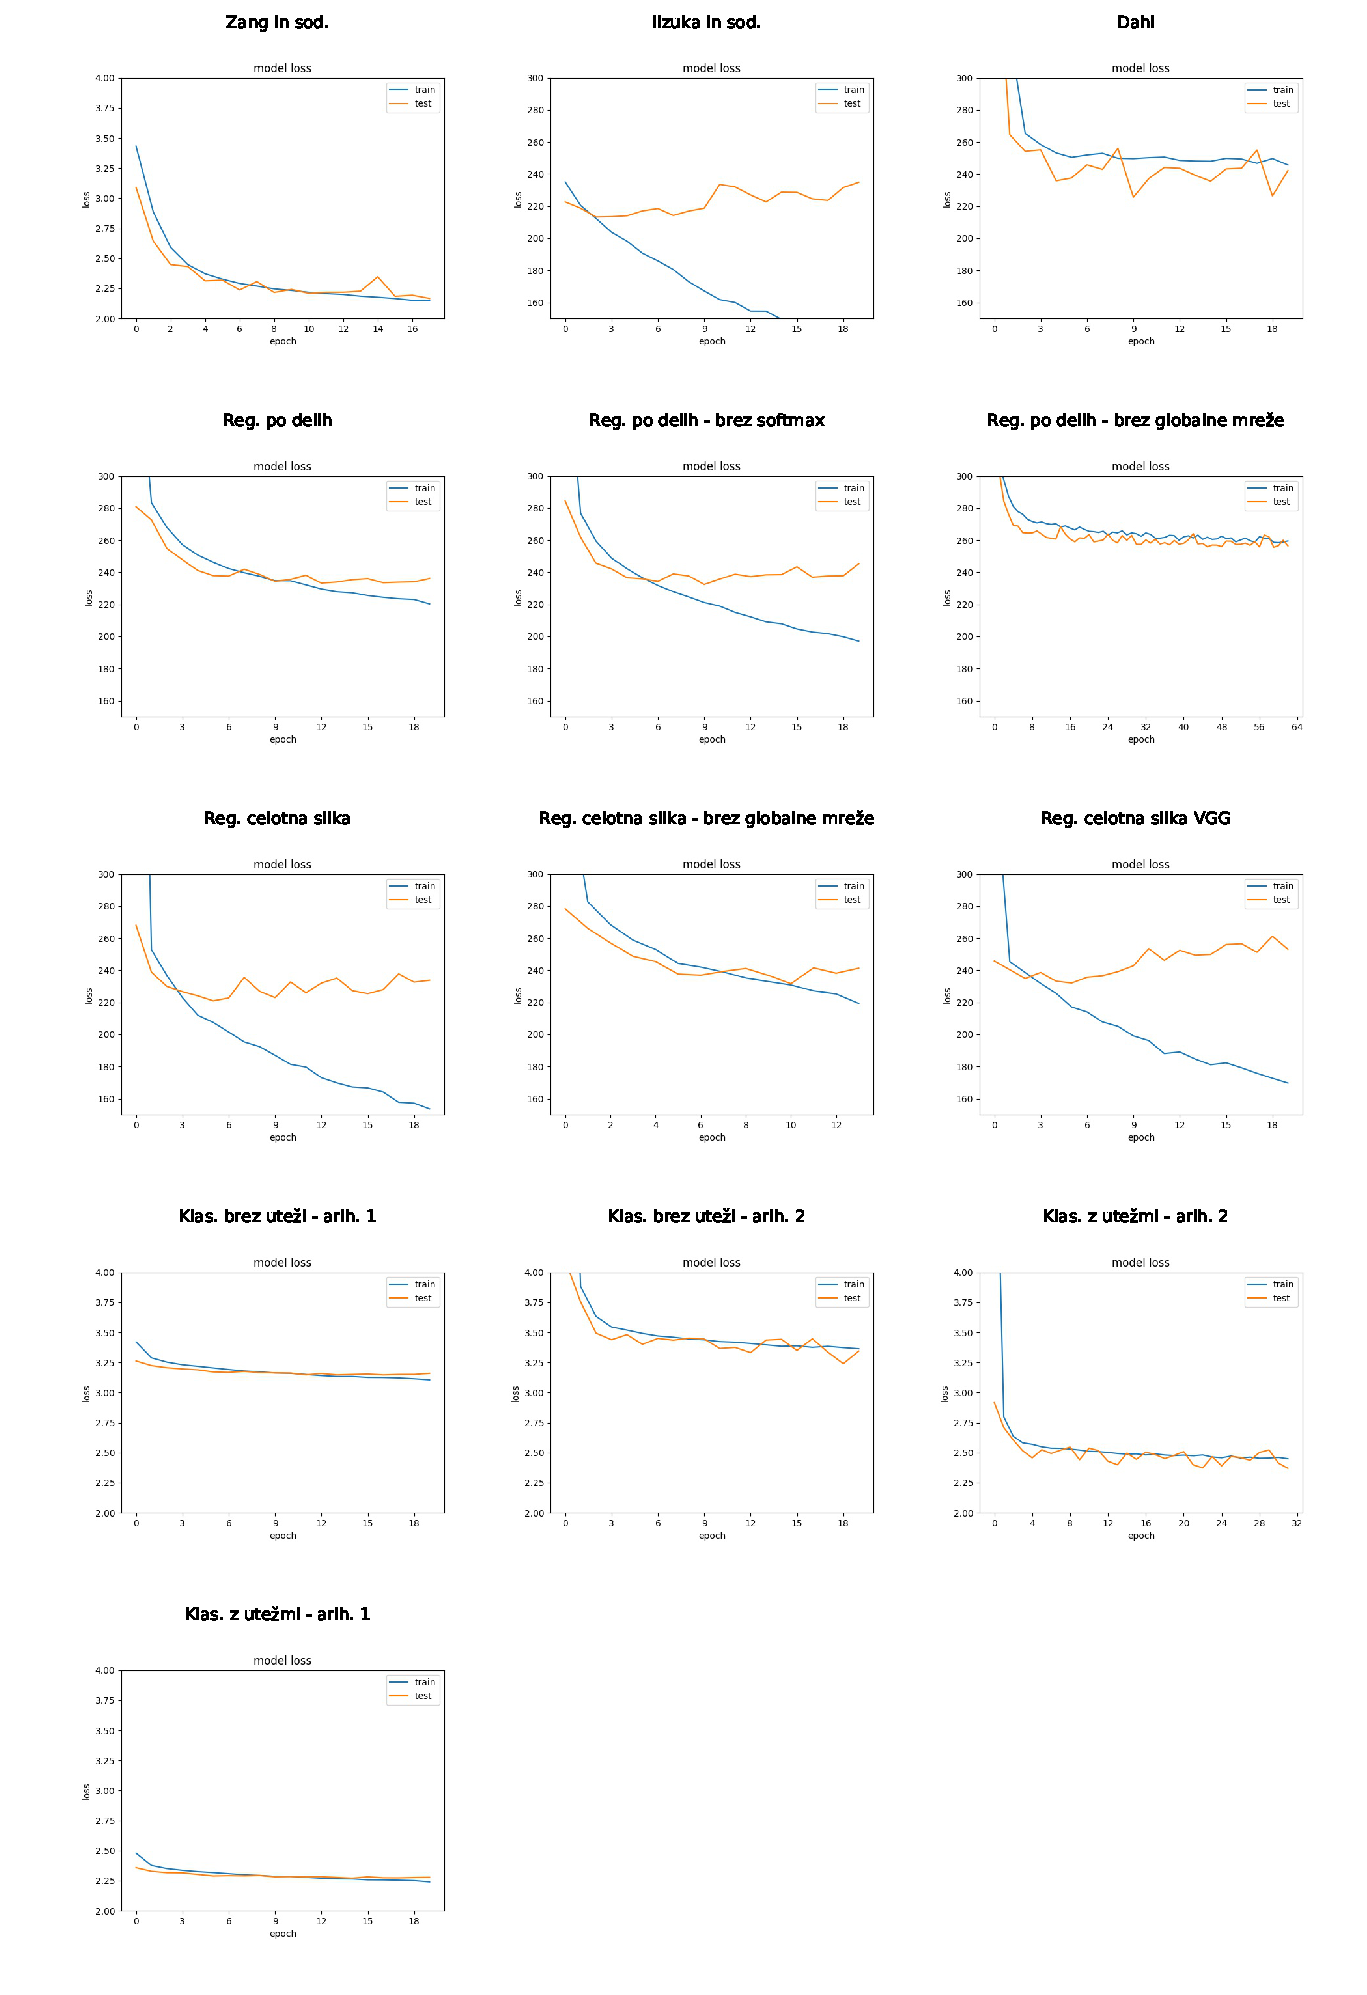
\includegraphics[width=12cm]{histograms-100}
\end{center}
\caption{Prikaz padanja napake modela pri učenju. Za vsak prehod preko vseh podatkov (ang. {\em epoch}) je prikazana vrednost cenilne funkcije na množici za treniranje in testni množici. }
\label{im:histograms-100}
\end{figure}

\subsection{Učenje na večji učni množici}


\subsection{Pomen nivojev mreže}


Konvolucjsko nevronsko mrežo si lahko predstavljamo, kot nivoje, ki poskrbijo za zajem značilk iz slike. V preteklosti so to počeli z različnimi pristopi kot so SIFT \cite{ke2004pca}, HOG \cite{ke2004pca}, SURF \cite{bay2006surf} in ostali. Nevronska mreža za to poskrbi, sama in izlušči tiste značilke, ki so za določeno nalogo relevantni. Uporabljene značilke lahko v grobem vidimo z vizualizacijo izhodov konvolucijskih nivojev. 
 
V tem poglavju bomo pogledali, katere značilke nivoji zaznajo v ta namen smo izrisali izhode prvih šestih konvolucijskih nivojev nevronske mreže, ki so prikazani na sliki \ref{im:layers-vis}. Vsak nivo predstavlja več slik, ki so izhodi posameznih filtrov, število slik je odvisno od števila filtrov. Čeprav ima mreža več nivojev smo se odločili, da prikažemo le prvih šest saj so ti najbolj razumljivi. Za vizualizacijo smo si izbrali pristop \textit{regresija celotna slika z globalno mrežo}, saj je ta najbolj primerna za to vizualizacijo.

Slike povejo na kaj se filtri v posameznem nivoju odzivajo oziroma kaj zaznajo. V prvem nivoju lahko opazimo, da se v večji meri osredotočajo na robove ali prehode med barvami v sliki. Opaziti je, da se nekateri odzovejo tudi na večji del slike in tako zgleda, kot da izhod kar osnovna slika. V drugem nivoju lahko opazimo že bolj osredotočene odzive. Nekateri še vedno zaznajo robove, drugi pa se že osredotočijo samo na določene dele slike na primer vodoravne robove. Nekateri zaznajo tudi že dele, ki se enako obarvajo na primer nebo v ozadju. 

V tretjem in četrtem nivoju je te osredotočenosti na določeno del ali motiv še več. Nekatere značilke je že težko razumeti in opisati. Še vedno je veliko filtrov, ki zaznavajo robove in površine, ki bodo kasneje enako obarvani. To se še vedno nadaljuje tudi v petem in šestem nivoju, kjer je še več značilk, ki imajo pomen za nevronsko mrežo, težje pa so razložljive nam ljudem. 

\begin{figure}[htb]
\begin{center}
\centering
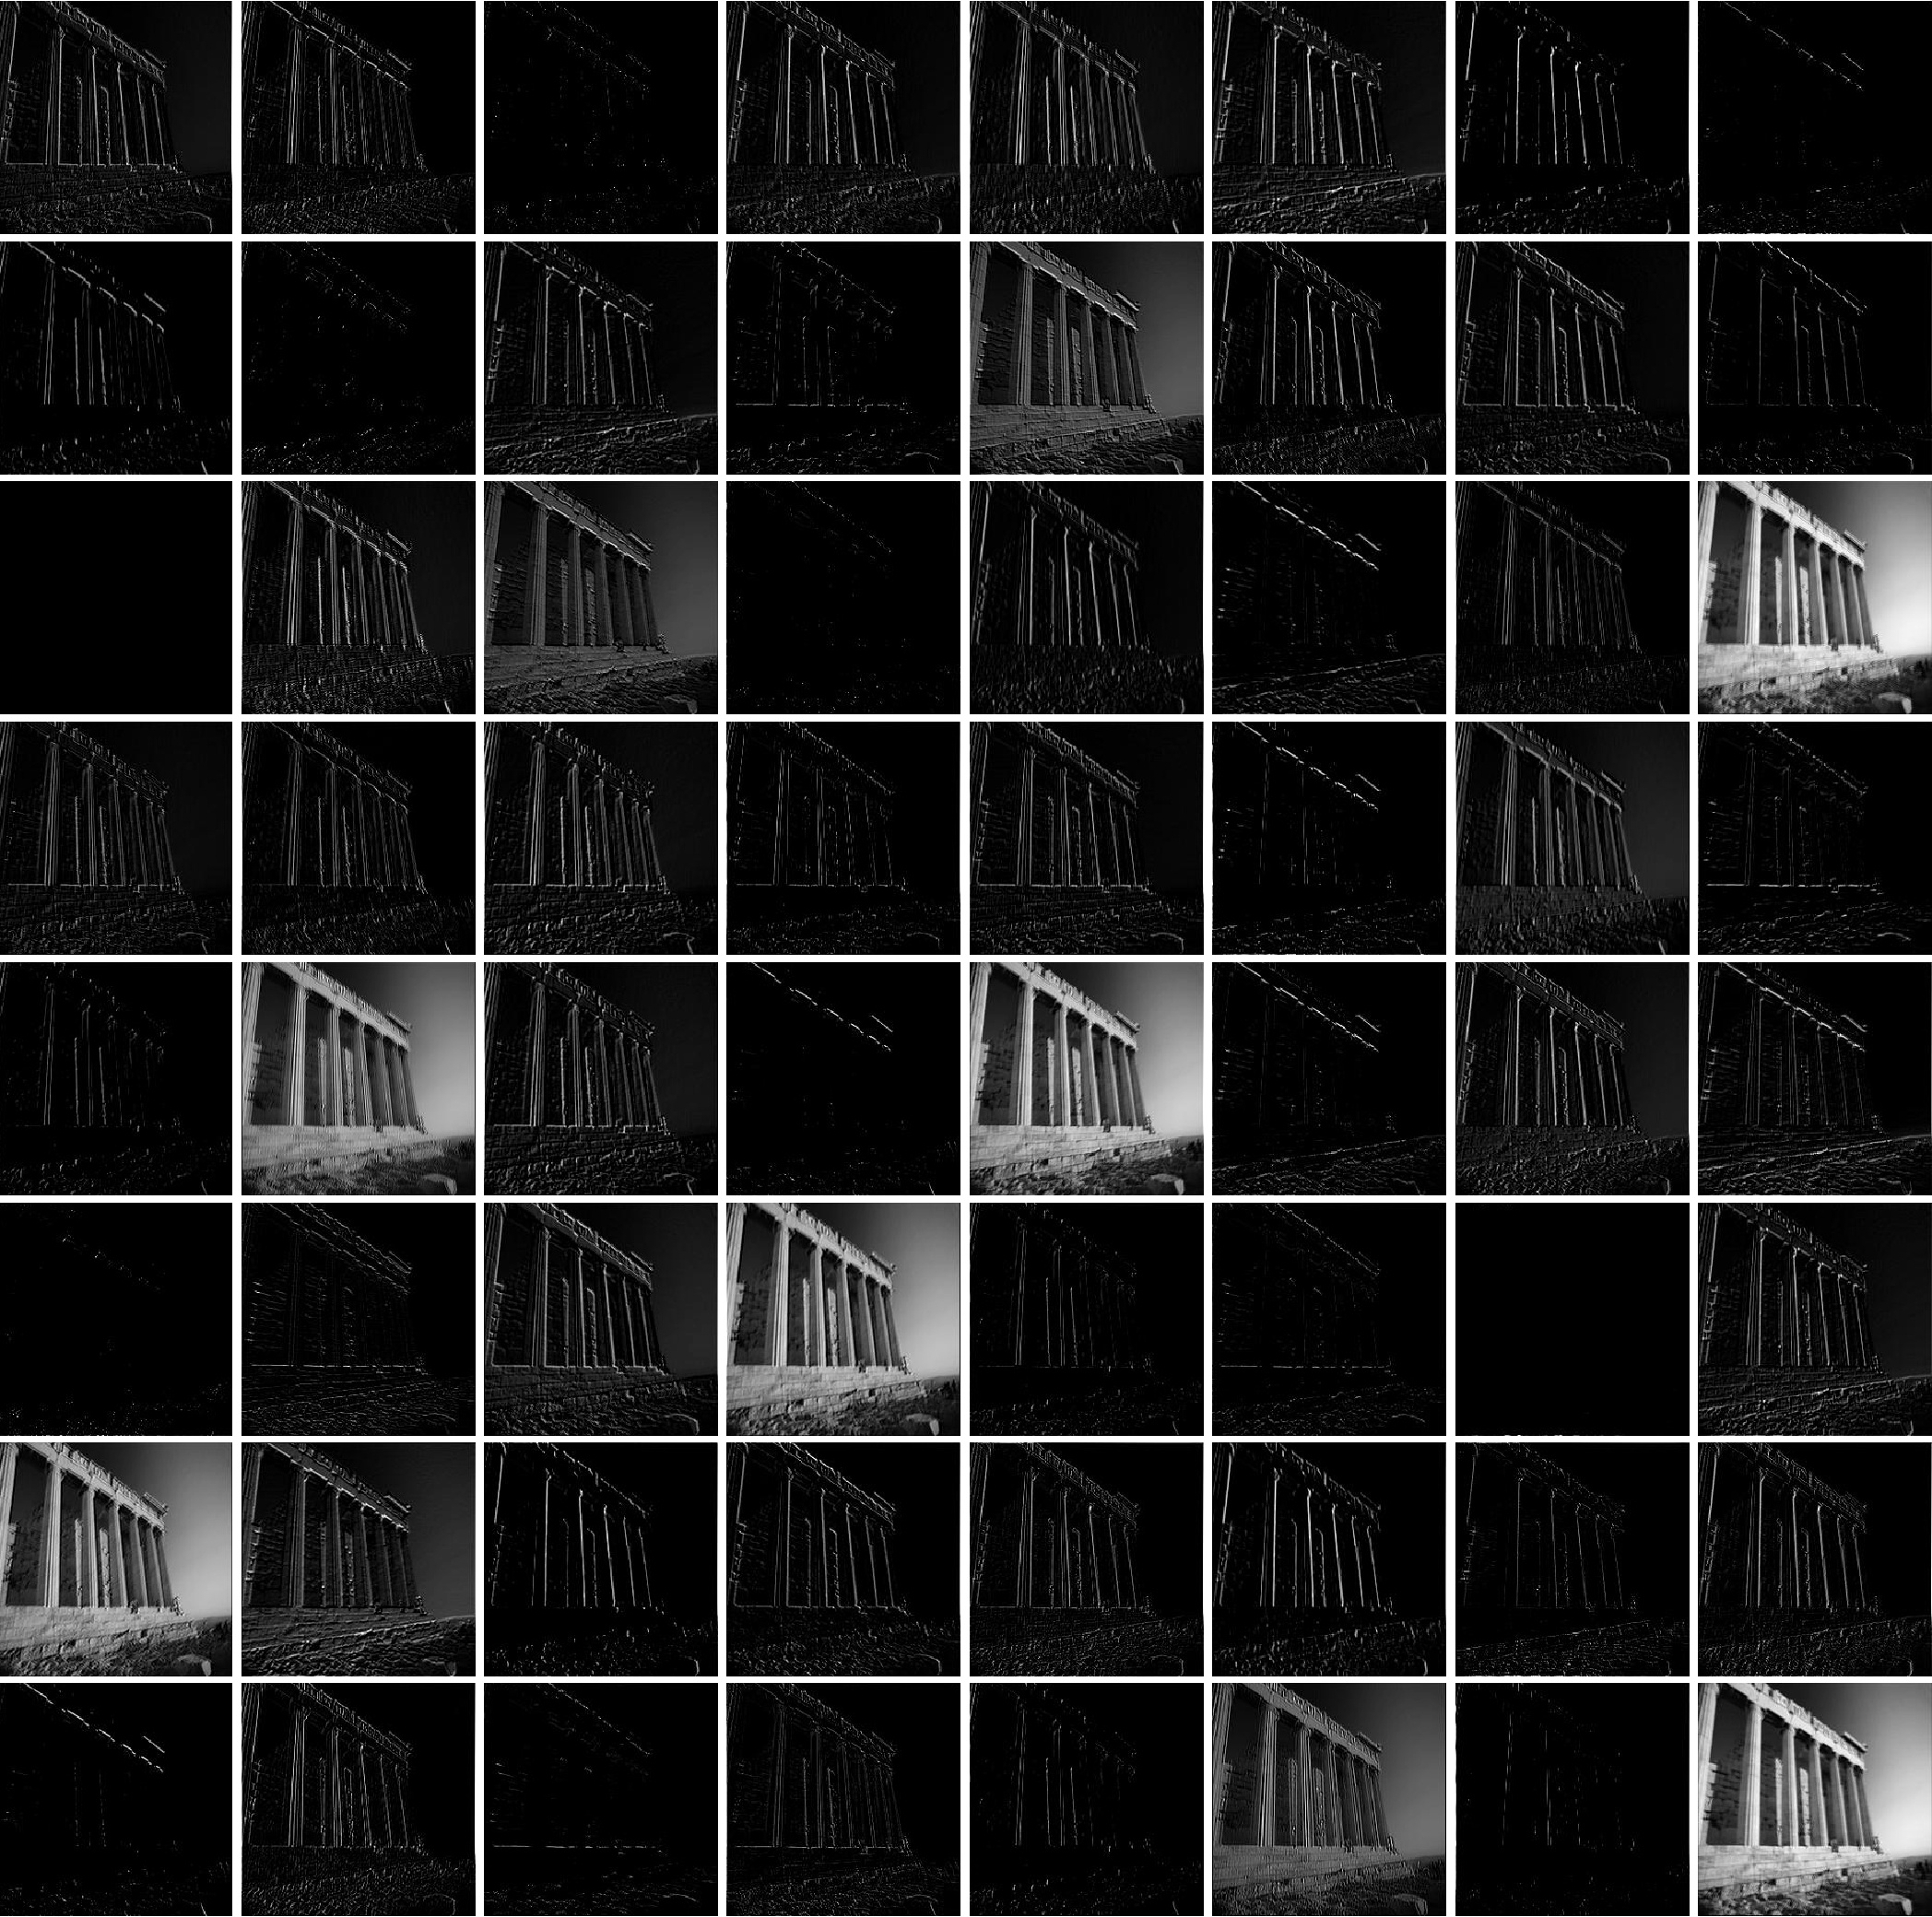
\includegraphics[width=6cm]{0_n03846431_2304}
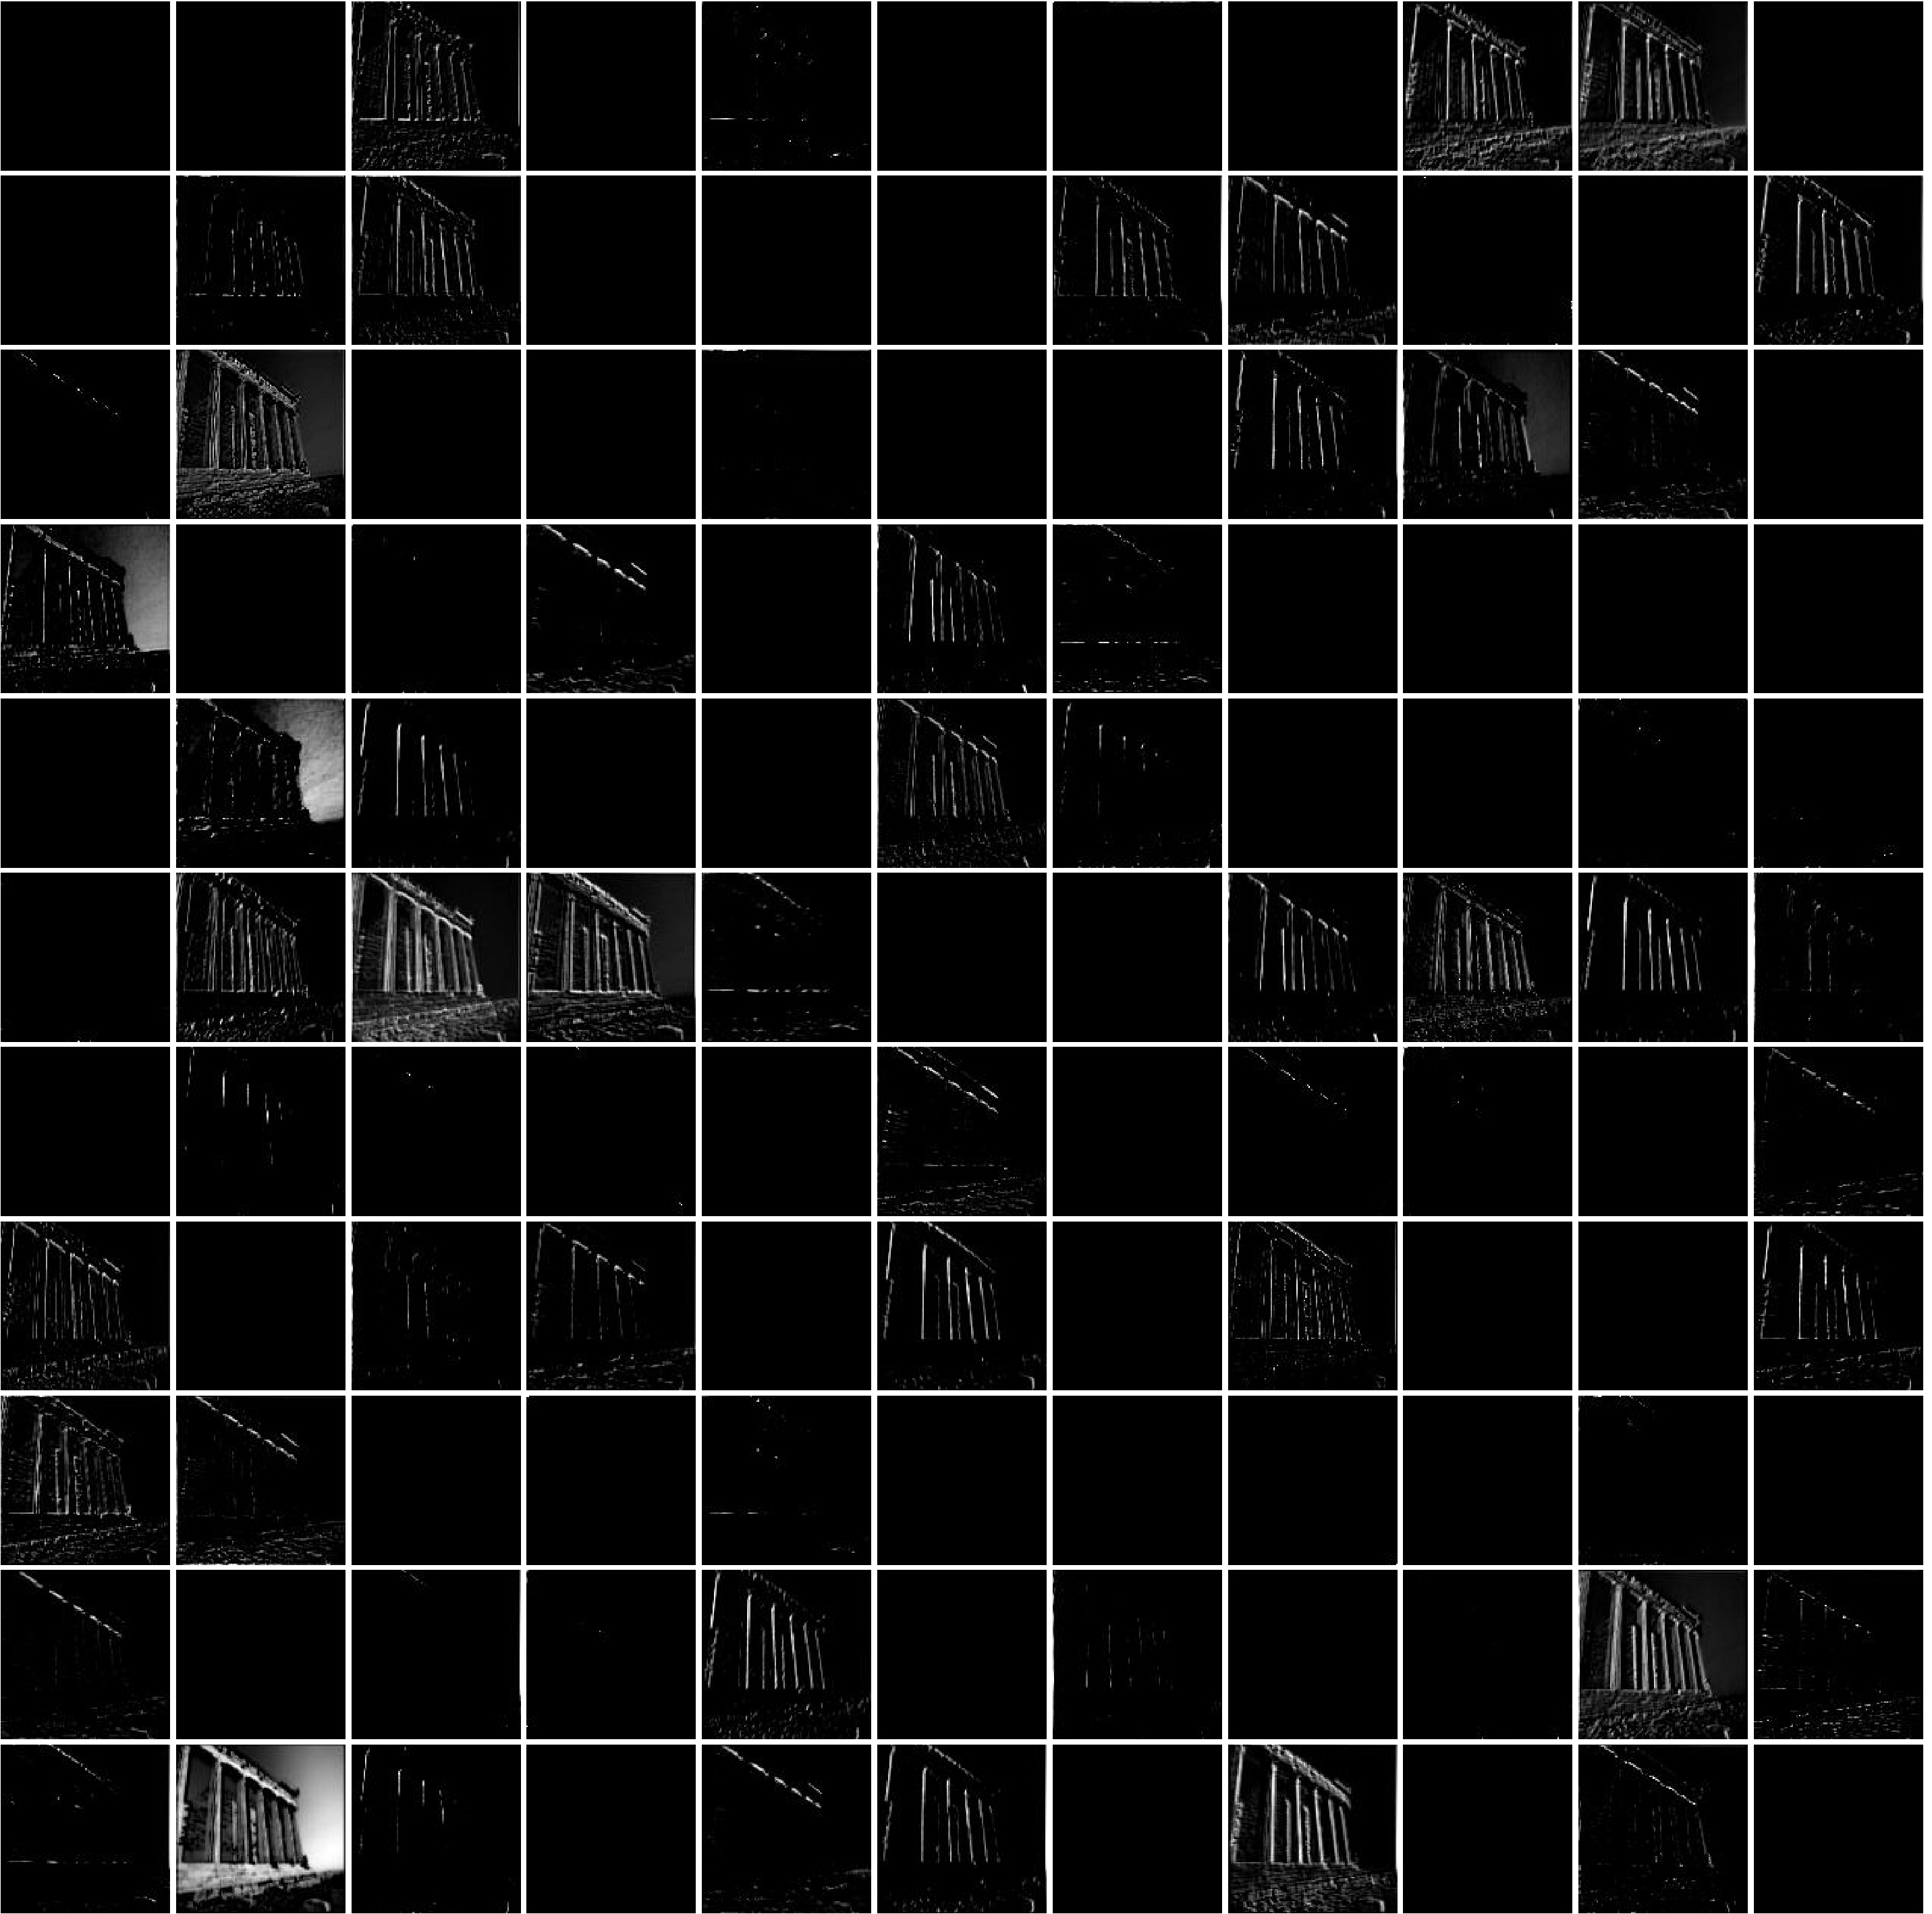
\includegraphics[width=6cm]{1_n03846431_2304}
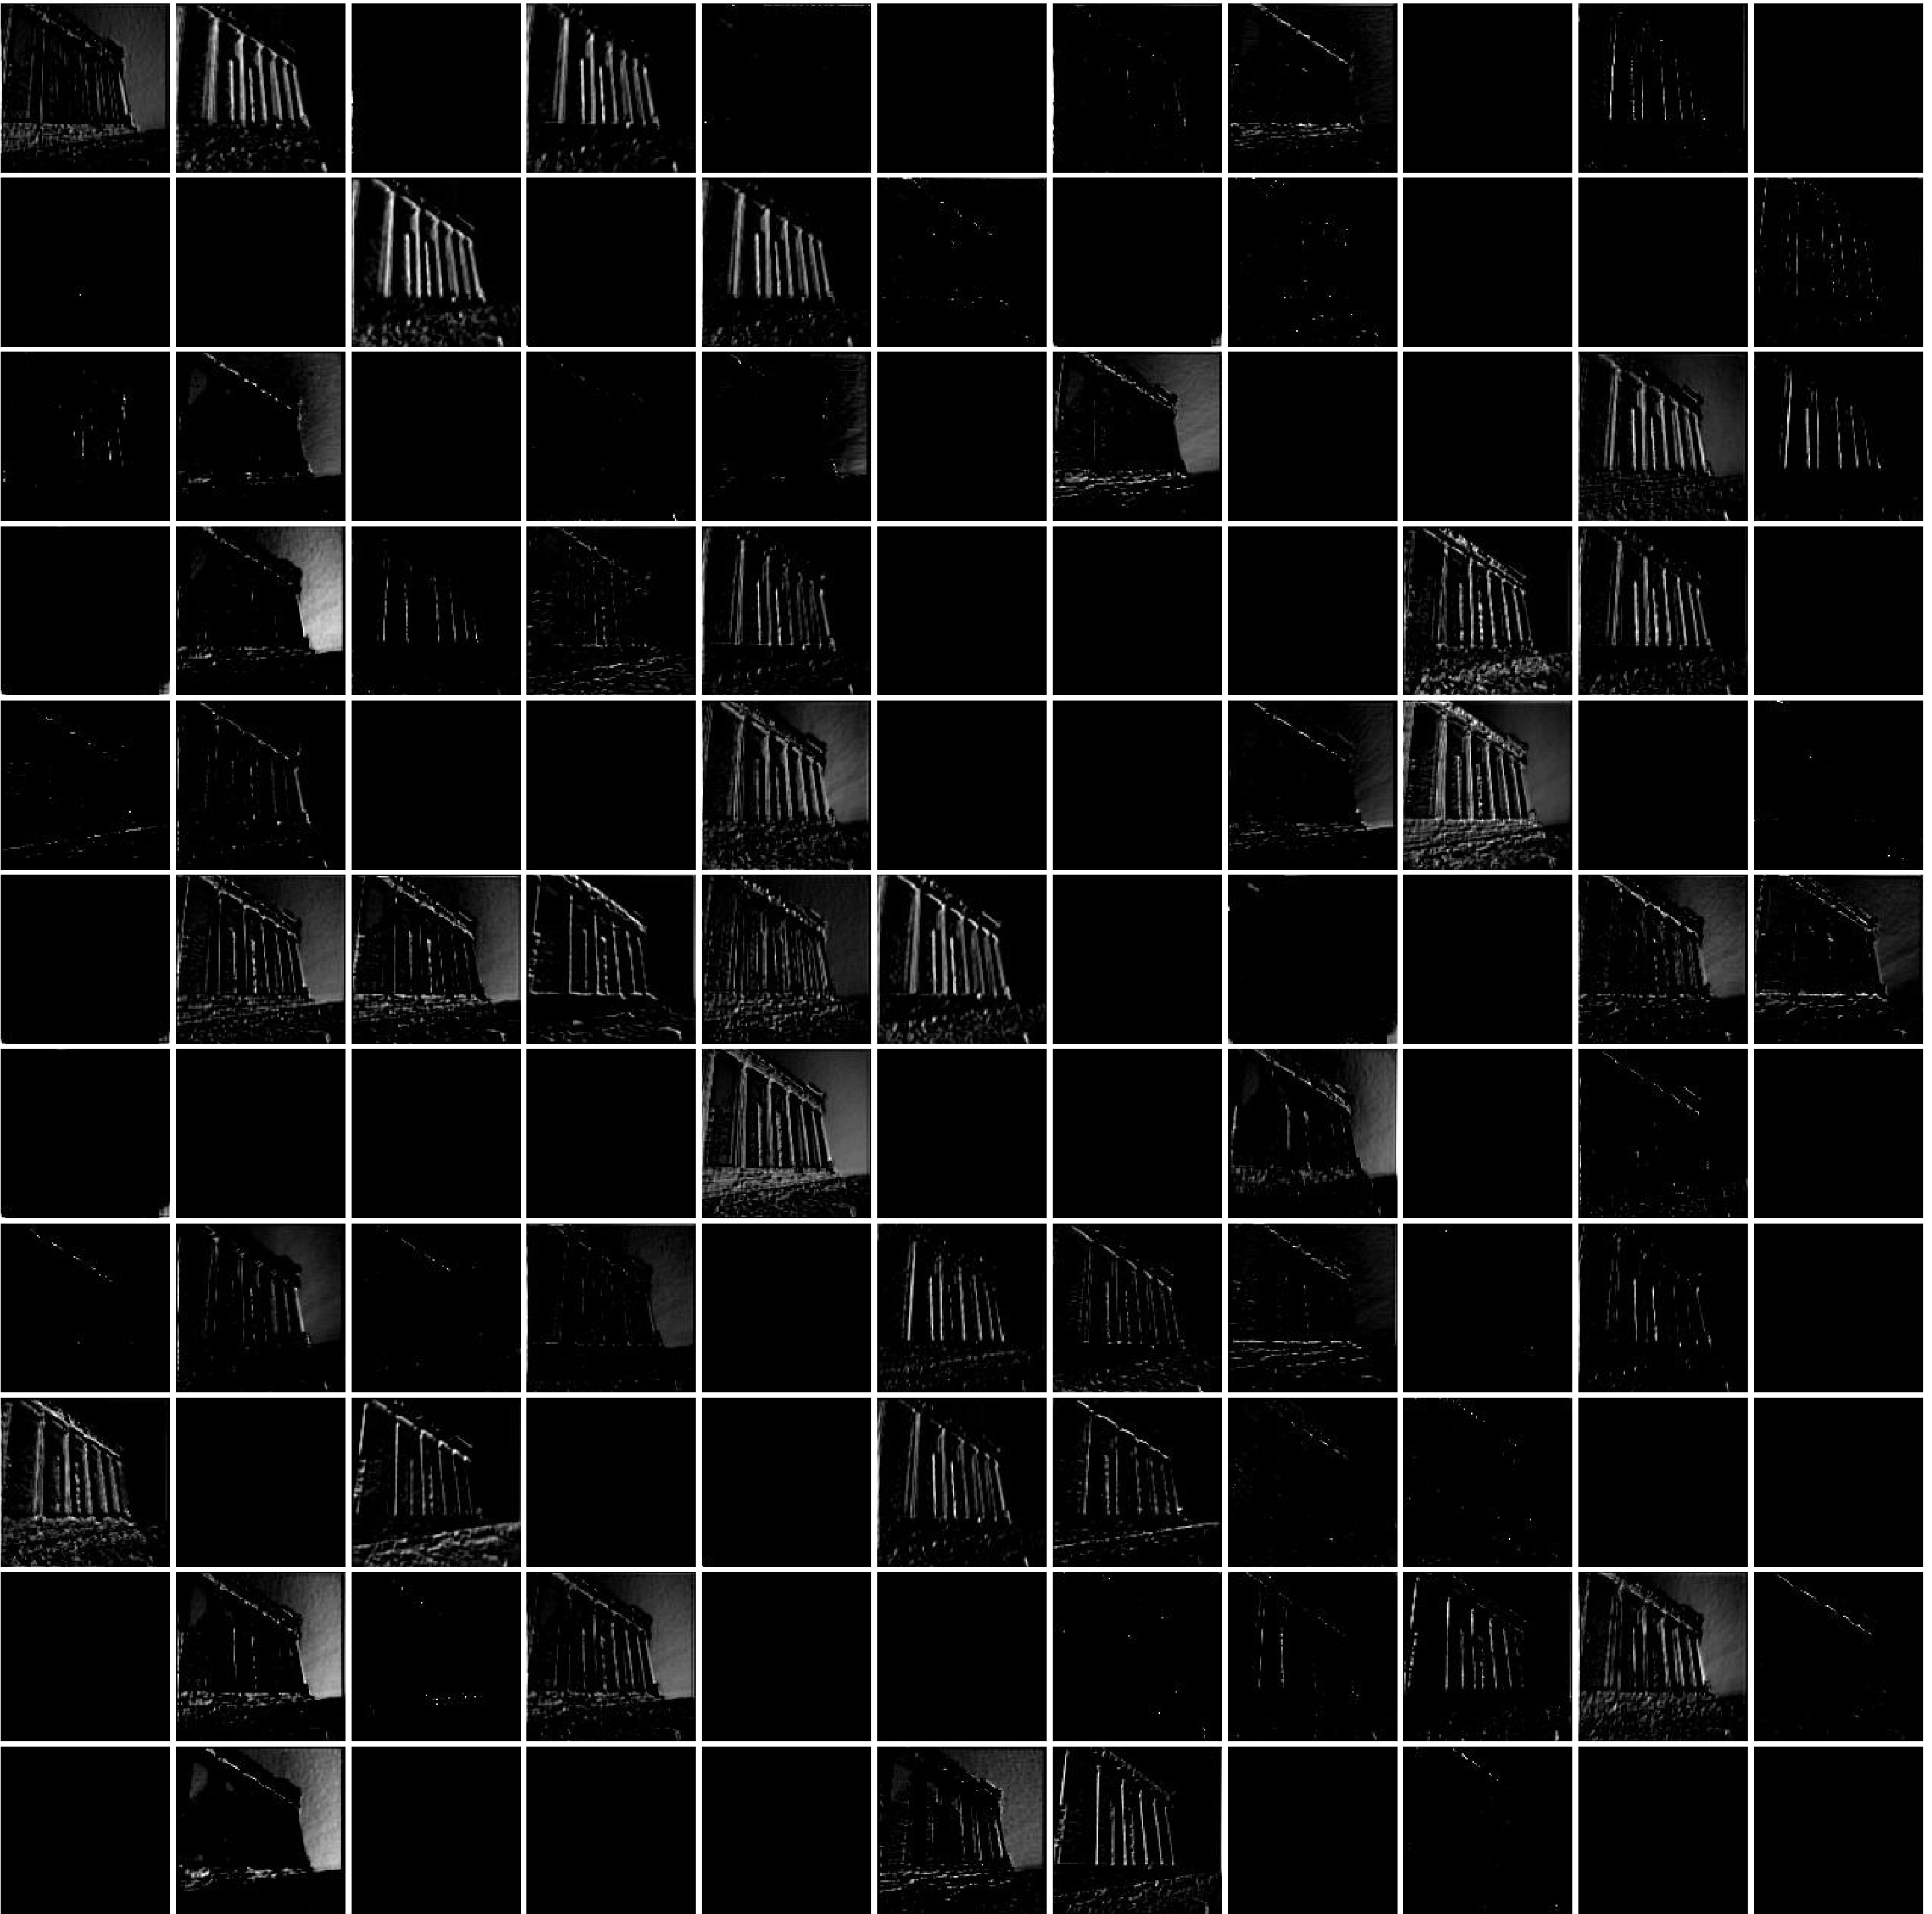
\includegraphics[width=6cm]{2_n03846431_2304}
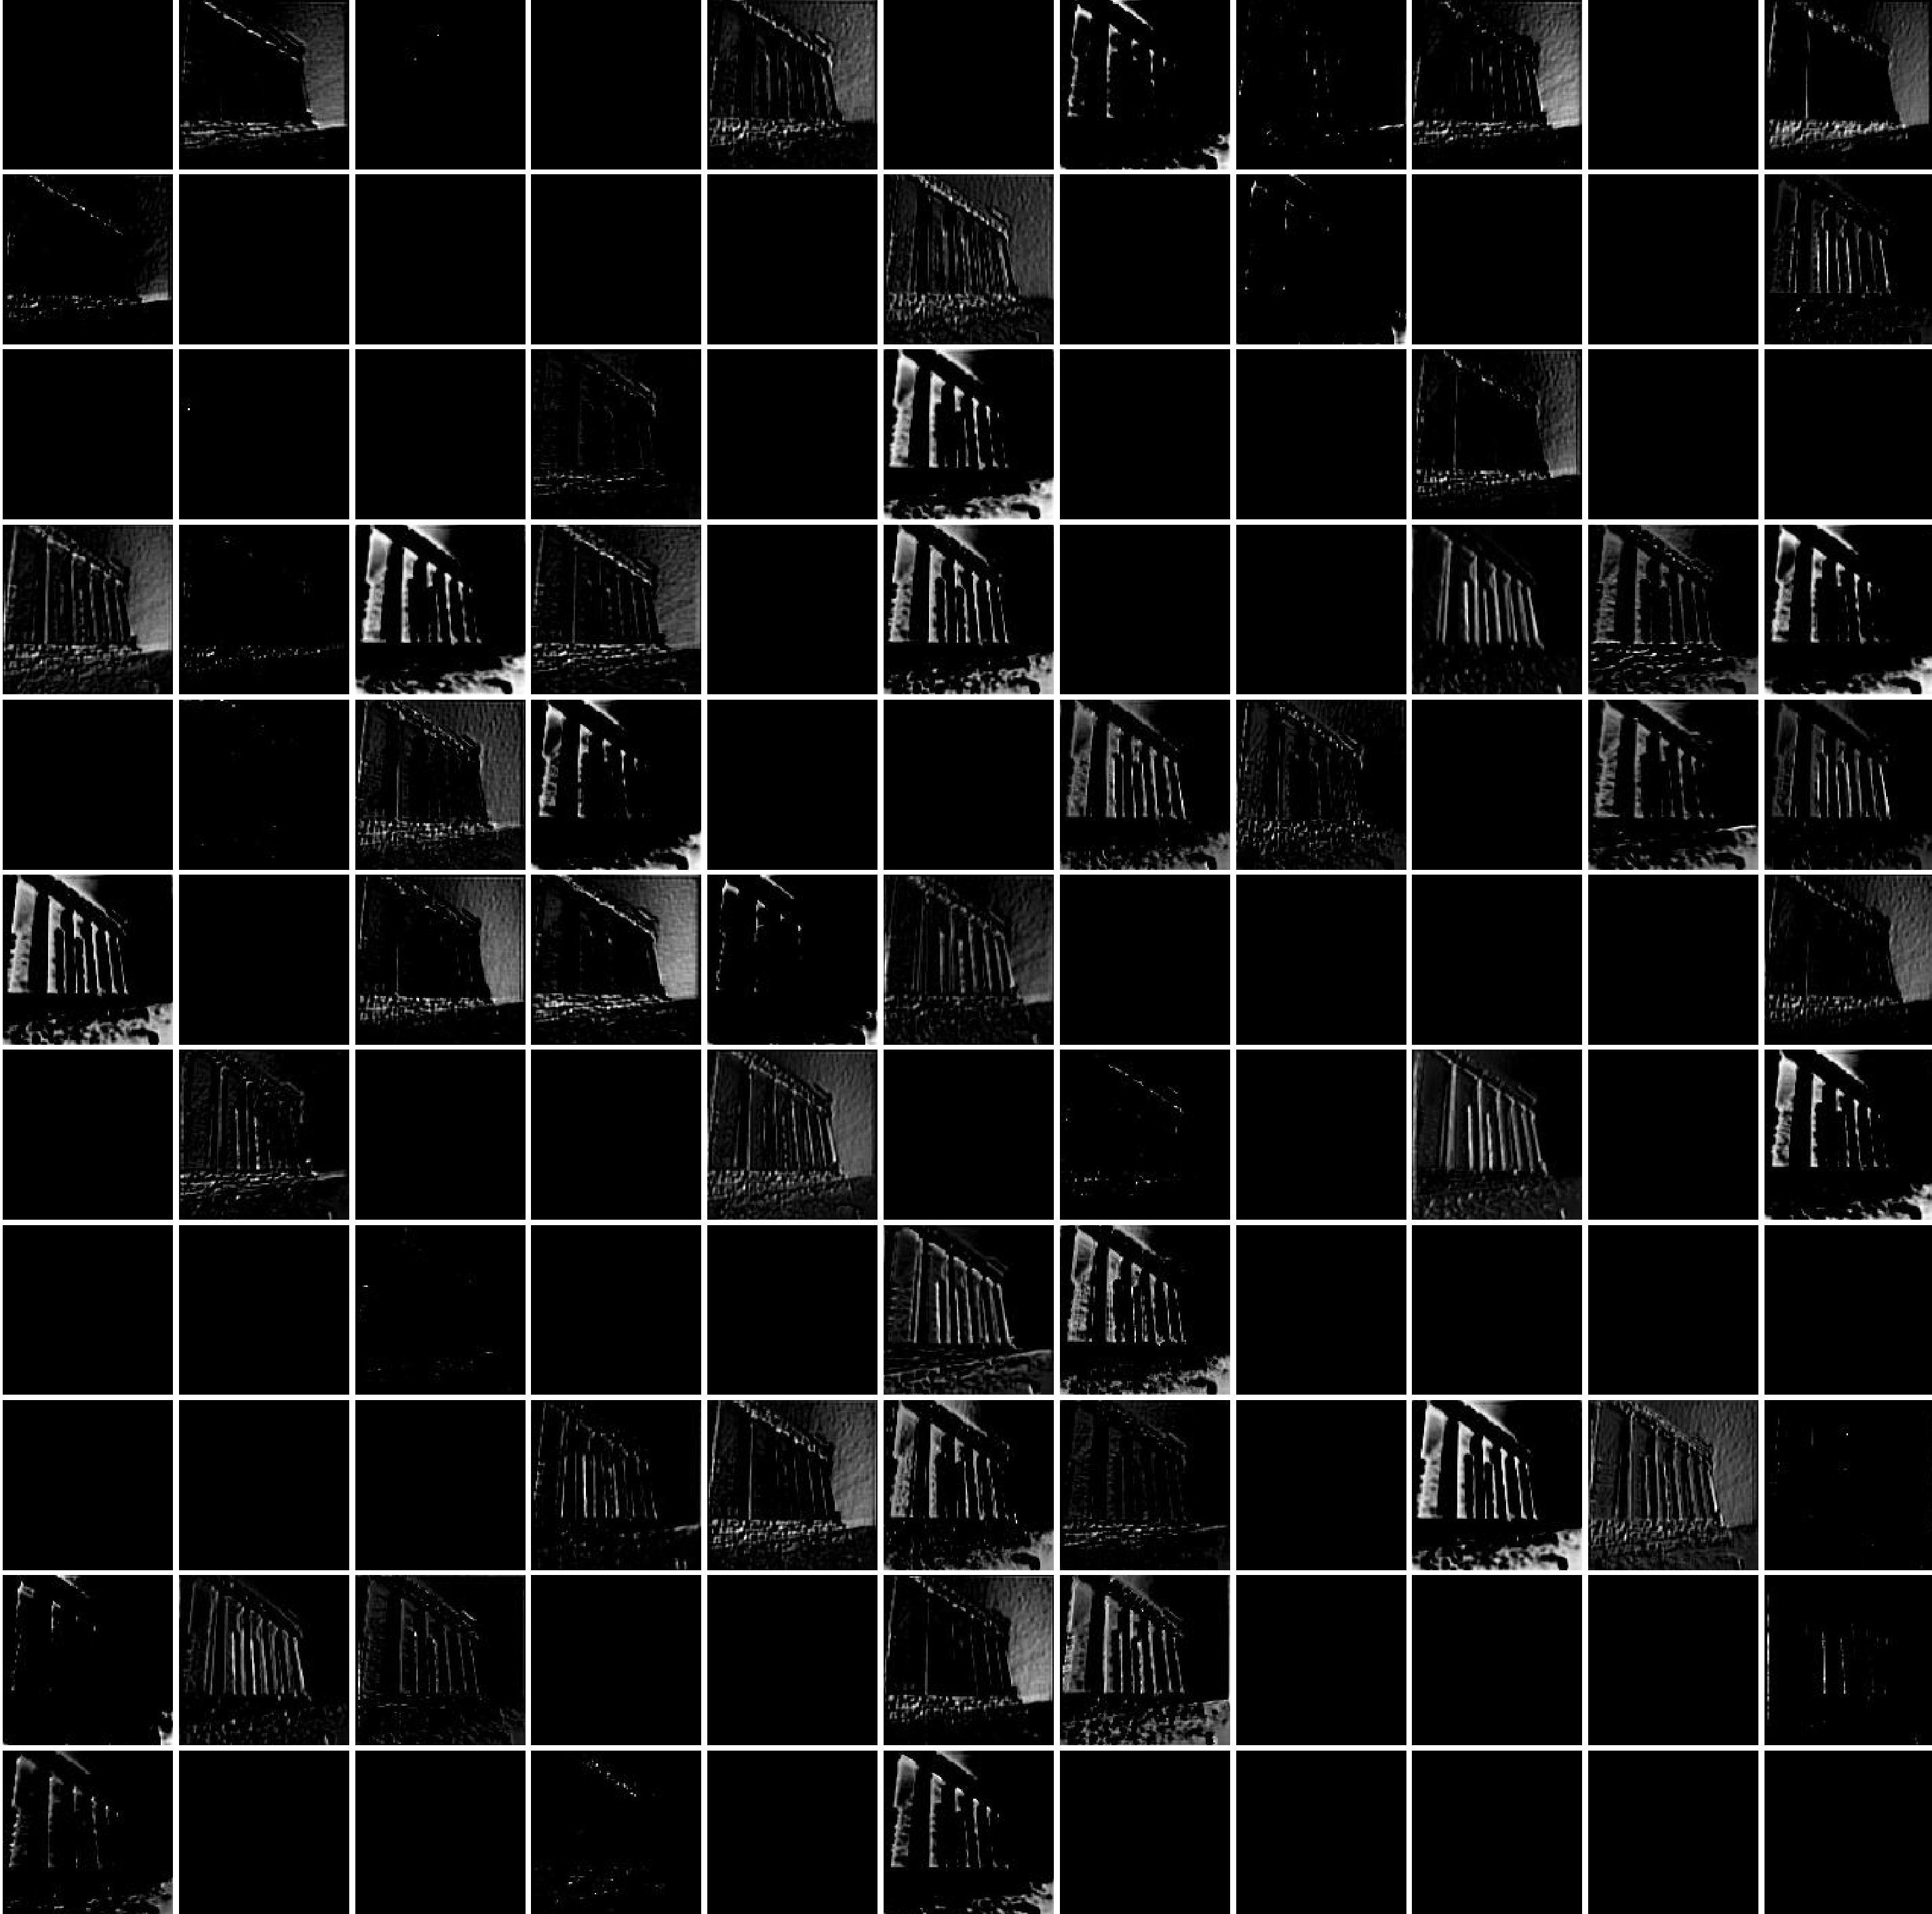
\includegraphics[width=6cm]{3_n03846431_2304}
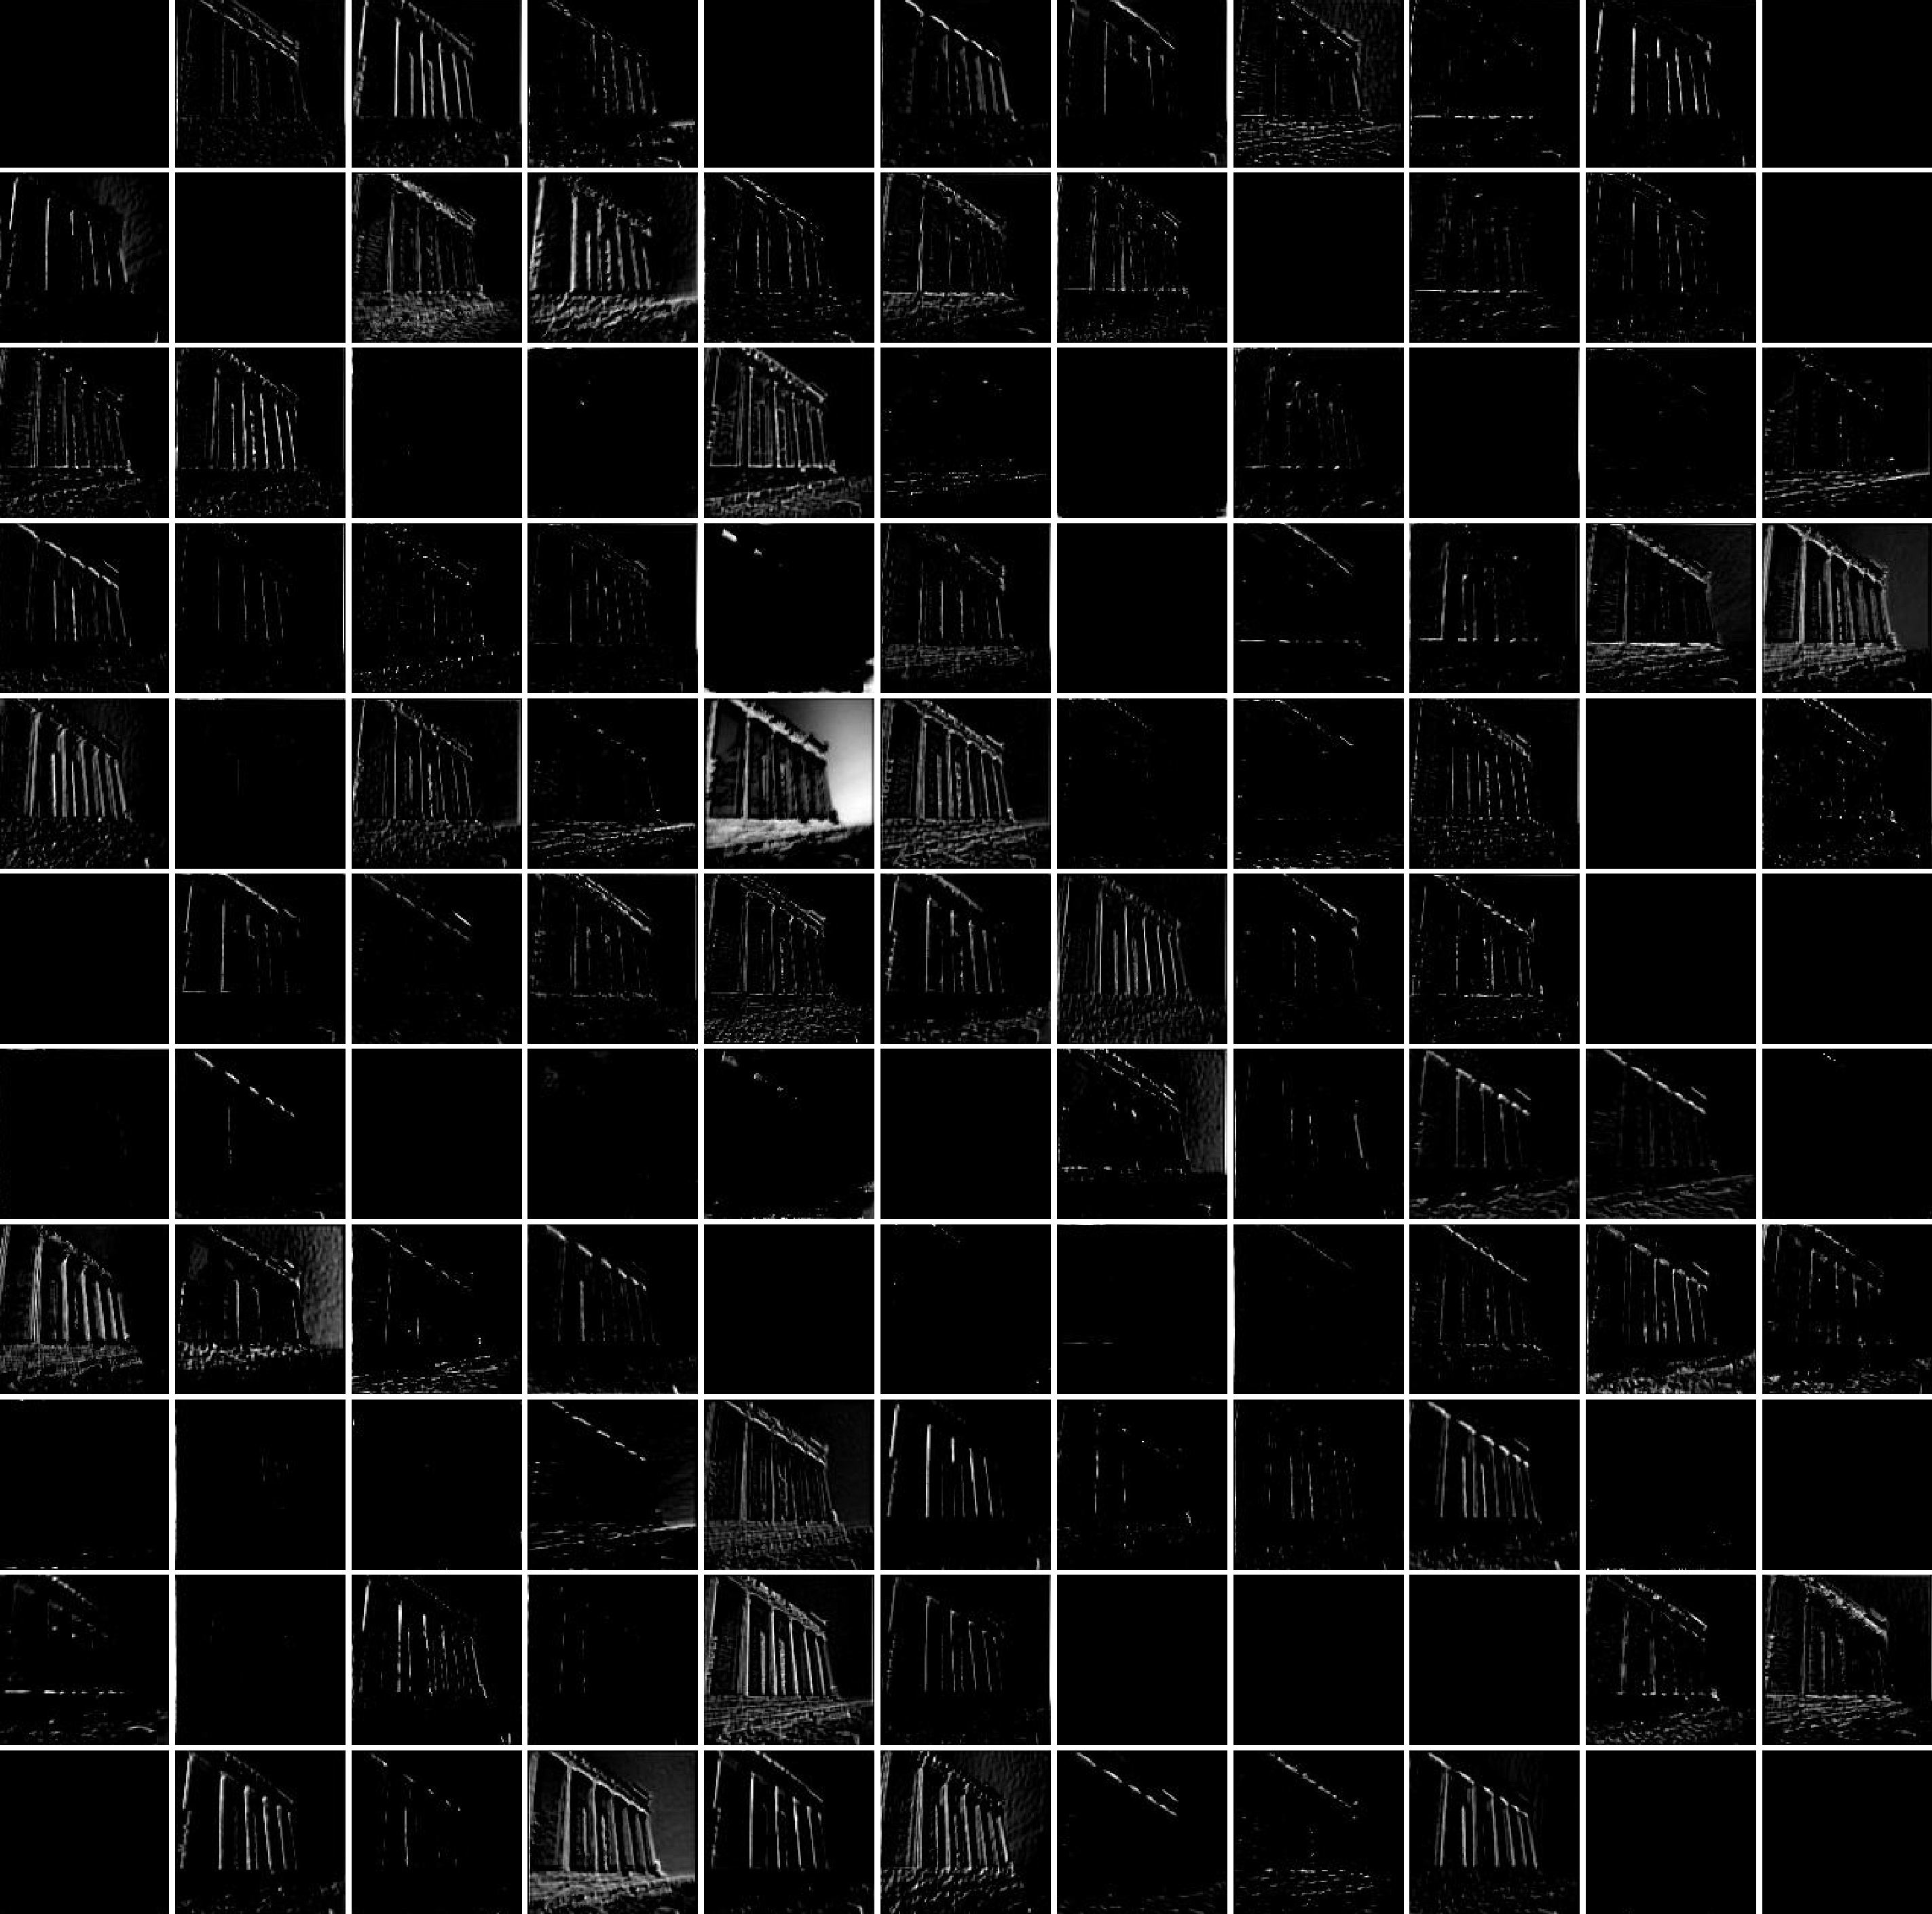
\includegraphics[width=6cm]{4_n03846431_2304}
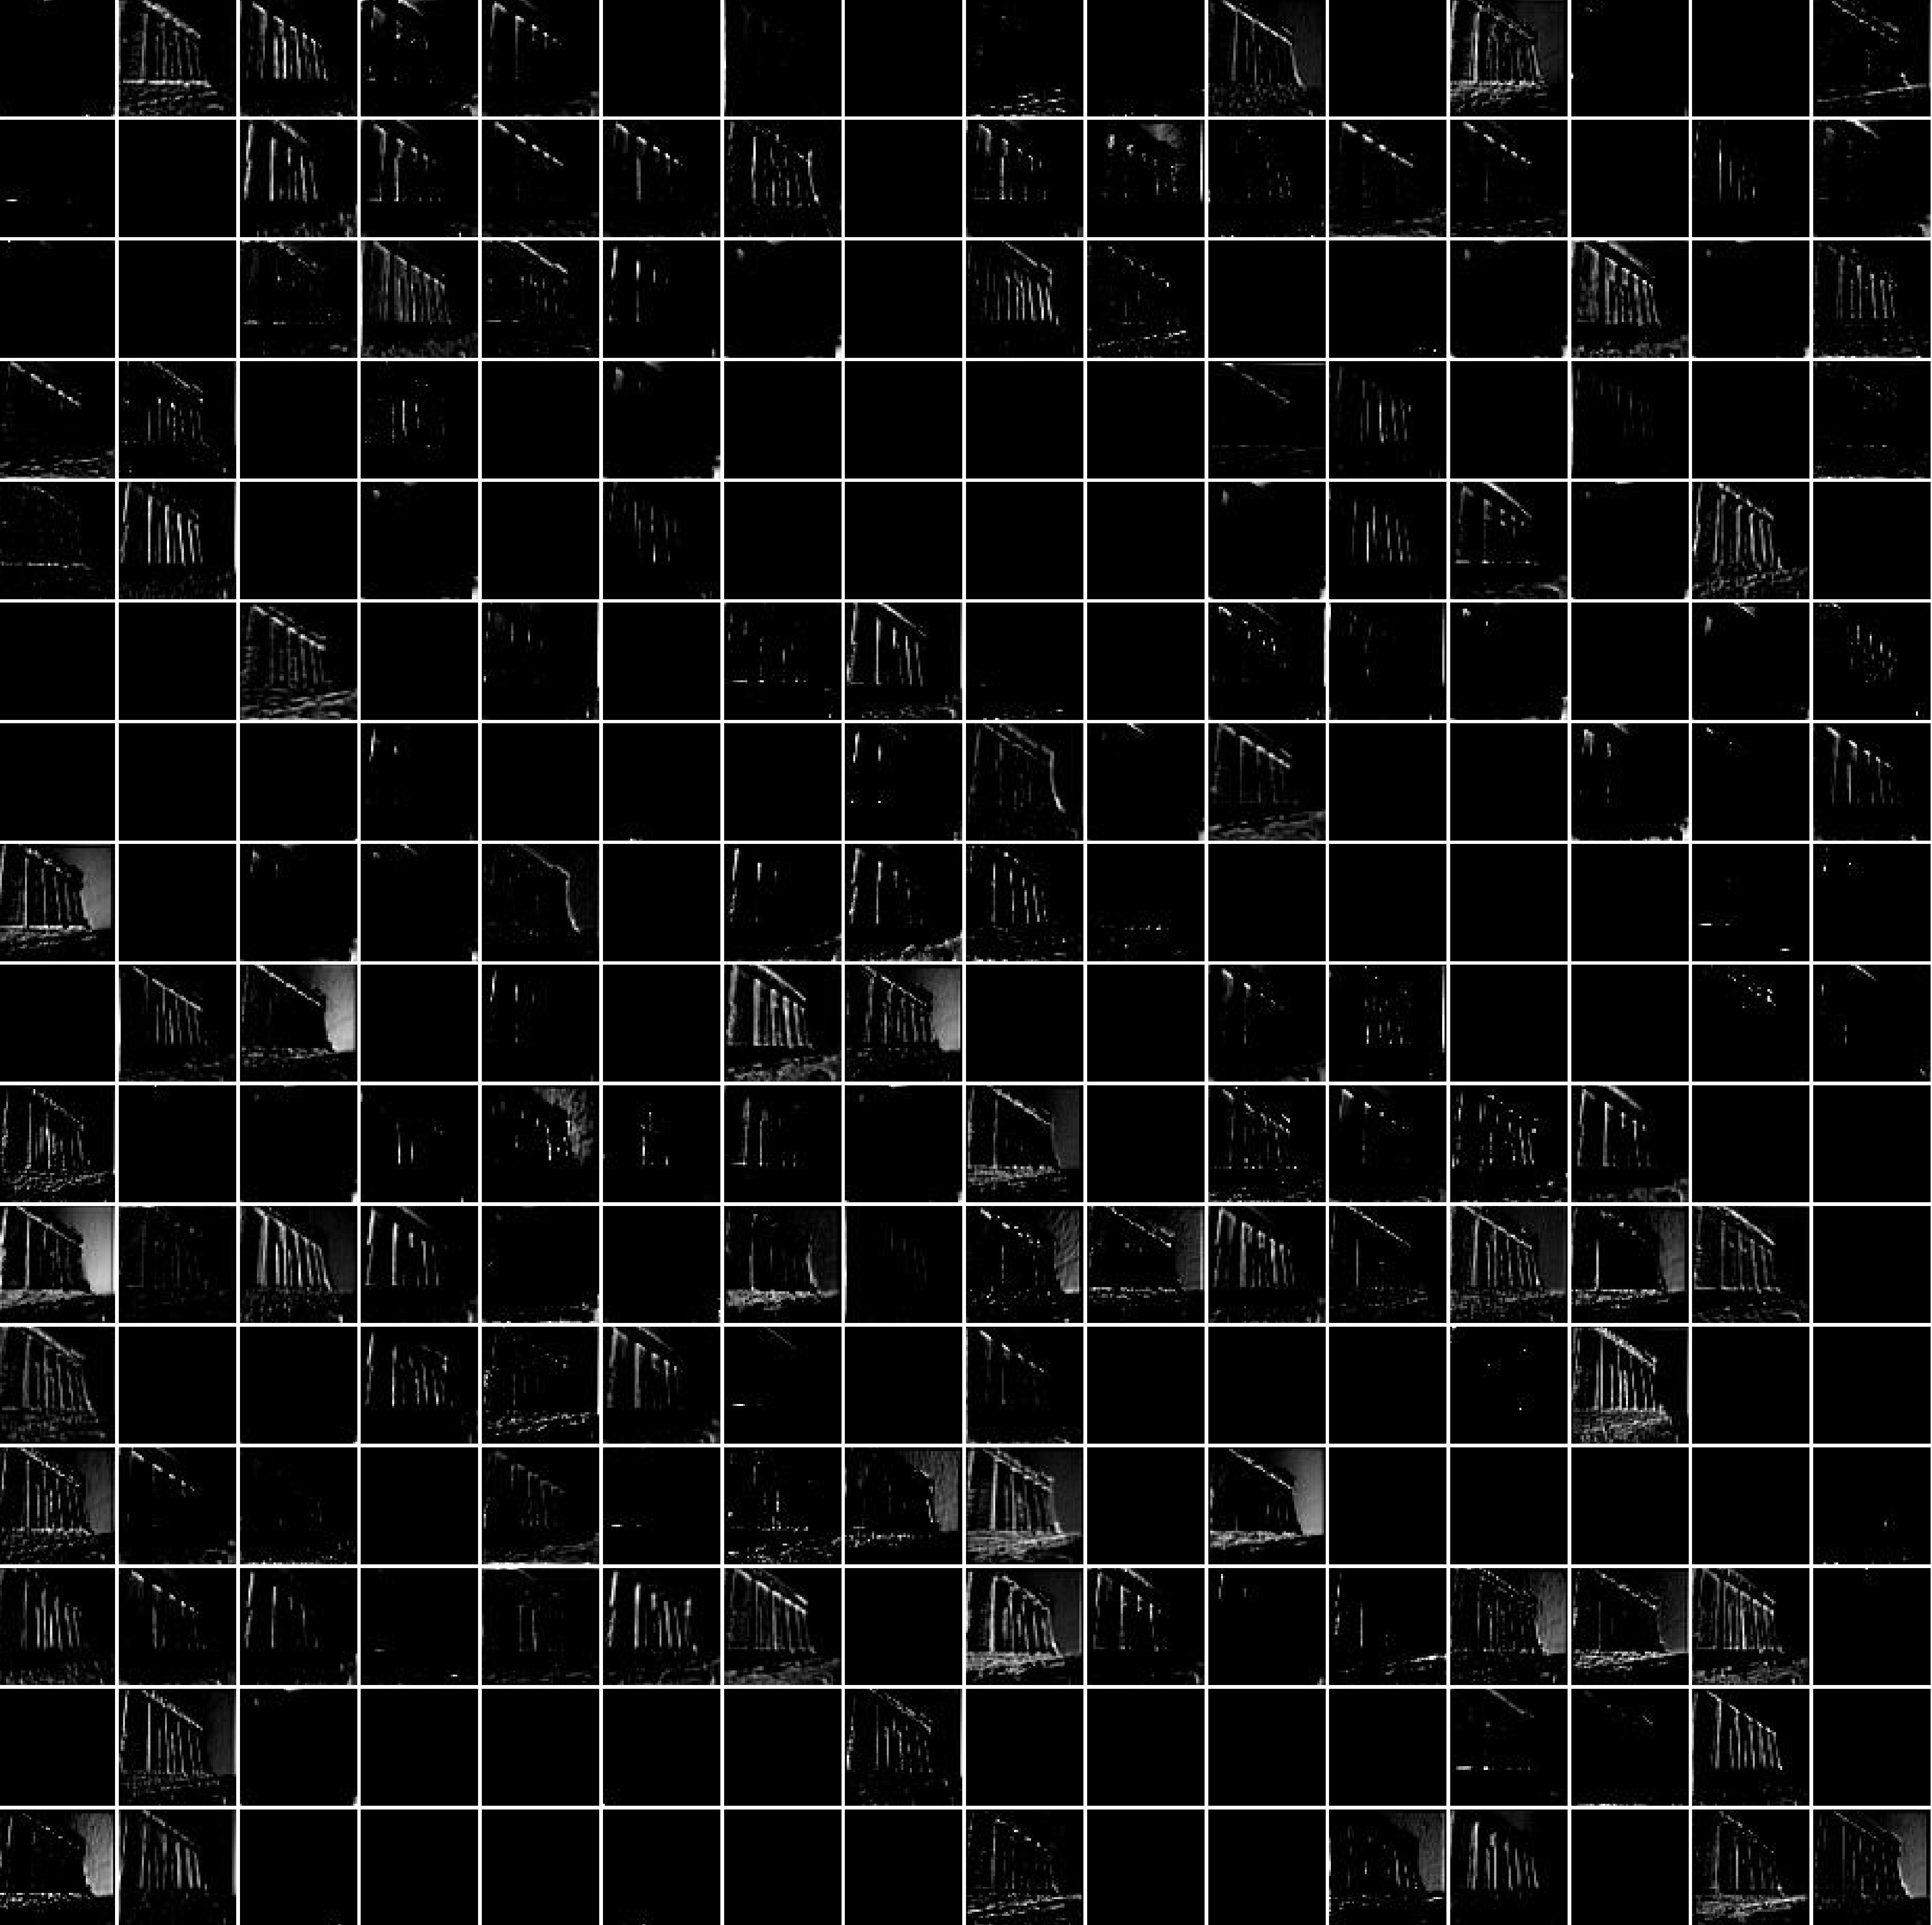
\includegraphics[width=6cm]{5_n03846431_2304}
\end{center}
\caption{Vizualizacija izhodov prvih 6 konvolucijskih nivojev nevronske mreže na primeru slike Atenske akropole. Slika prikazuje kaj v sliki zaznajo posamezni nivoji in posamezni filtri.   }
\label{im:layers-vis}
\end{figure}



%----------------------------------------------------------------
% Section: Podatki
%----------------------------------------------------------------

\section{Barvanje večjih slik}
\label{ch:vecjih}

Večina pristopov v sorodnih delih je naučenih za barvanje slik velikosti $224 \times 224$. Večina pristopov ima to omejitev, da omogoča le barvanje slik te velikosti. Iizuak in sod. \cite{Iizuka2016} omogočajo barvanje večjih slik, tako da večjo sliko podamo enaki mreži na vhod, ki nima omejitev v velikost, saj je sestavljena le iz konvlucijskih nivojev. Pri tem je komentar avtorjev, da mreža deluje bolje na slikah velikosti $224 \times 224$.

Z pristopih po delih, ki smo jih implementirali v okviru tega dela, ta problem rešujemo drugače. Sliko katerekoli velikosti večje od $32 \times 32$ razdelimo na dele velikosti $32 \times 32$ s prekrivanjem, jo obarvamo po delih in potem spet sestavimo po principu opisnem v poglavju \ref{ch:parts-im}.

Primerjavo kakovosti barvanja večjih slik smo izvedeli tako, da smo pristopa \textit{Iizuka in sod.} ter \textit{regresijo po delih z globalno mrežo} preizkusili na istih slikah pomanjšanih na  velikost $224 \times 224$ slikovnih točk, kjer naj bi bilo barvanje optimalno in velikost $896 \times 896$. Primerjava je izvedena na mrežah naučenih na manjši učni množici s $100 000$ slikami. 


\section{Podatki}

Podatke, ki smo jih uporabili v za treniranje in validacijo pristopov smo pridobili iz podatkovne zbirke ImageNet \cite{ILSVRC15}, ki vsebuje približno $14$ milijonov slik. Iz zbirke smo naključno izbrali množico podatkov jih za namen učenja pretvorili v \textit{CIE L*a*b*} barvni prostor. Pri preizkusu na manjši množici smo za učenje naključno izbrali $100 000$ slik za vlidacijo pa $10 000$ slik iz nabora. Validacijska množica je bila obenem tudi testna množica. 

Za namen testiranja barvanja večjih slik opisanega v poglavju \ref{ch:vecjih} podatki iz podatkovne zbirke \textit{Imagenet} niso bili zadovoljivi, saj so slike večinoma velikosti manjših od $500 \times 500$ slikovnih točk. Odločili smo se, da testiranje izvedemo na lastnih slikah, ki večje od velikosti $896 \times 896$, kar pomeni, da slik ni potrebno povečevati in s tem povzročati dodatnih napak v barvanju zaradi slabe kvalitete slik. Za namen testiranja smo vzeli 584 slik, katere je aplikacija \textit{Google Photos}\footnotemark ocenila, da gre za slike pohodništva. Za te slike pohodništva smo se odločili, ker gre večinoma za slike narave, kjer je barvanje ponavadi najboljše in lahko tako razliko opazujemo na slikah, ki se po navadi barvajo dobro. 

\footnotetext{\url{http://photos.google.com}}

%----------------------------------------------------------------
% Section: Podatki
%----------------------------------------------------------------

\section{Računanje napake}
\label{ch:napake}

Za primerjavo metod smo napake računali na validcacijski množici. Pri tem smo uporabili dve metrike: kvadratni koren povprečne napake (ang. {\em Root mean squeared error}) in razmerje med signalom in šumom (ang. {\em Peak signal-to-noise ratio}).  

Kvadratni koren povprečne napake (RMSE) za vsako sliko smo izračunali s pomočjo enačbe \ref{eq:rmse}, kjer $w$ in $h$ prestavljata širino in višino slike ter $c$ predstavlja število kanalov slike.  $d$ je originalna slika (ang. {\em ground truth}) in $\hat{d}$ obarvana slika. Napaka je bila izračunana za vsako sliko posebej in kasneje povprečena preko vseh slik. Napaka RMSE je bila izračunana na slikah v CIE L*a*b* barvnem prostoru le za $a*$ in $b*$ barvni kanal, saj za $L*$ barvni kanal izračun napake ni smiseln, ker so vrednosti vzete iz originalne slike. 

\begin{equation}
RMSE = \sqrt{\sum^{w}_{i=1} \sum^{h}_{j=1} \sum^{c}_{k=1} (d_{i, j, k} - \hat{d}_{i, j, k})}
\label{eq:rmse}
\end{equation} 

Razmerje med signalom in šumom (PSNR) je metrika, ki kaže razmerje med največjo možno močjo signala in močjo šuma, ki signal pokvari. Primerna je za primerjave rekonstruiranih podatkov, kot so v našem primeru validacijske slike, ki jih poskušamo rekonstruirati s pomočjo nevronske mreže. Vrednosti razmerja med signalom in šumom se merijo v enoti decibel (dB) \cite{Saupe2006}. Zadovoljive vrednosti rekonstrukcije slike 8 bitnih podatkov, kar naši podatki so, saj smo primerjali slike v barvnem prostoru \textit{RGB}, je med $30$ in $50$ dB \cite{welstead1999fractal}. 

Napako PSNR smo izračunali z enačbo \ref{eq:psnr}, v kateri ima $MAX_I$ največjo možno vrednost slikovne točke, kar je v barvnem prostoru RGB $255$, $RMSE$ pa je napaka izračuana z enačbo \ref{eq:rmse}. Napako smo povprečili preko vseh slik v testni množici. 

\begin{equation}
PSNR = 20 \log_{10}\left(\frac{MAX_I}{RMSE}\right)
\label{eq:psnr}
\end{equation}


%----------------------------------------------------------------
% Poglavje (Chapter) 5: Rezulatati in diskusija
%----------------------------------------------------------------

\chapter{Rezultati in diskusija}ž
\label{ch:rezultati}

\section{Primerjava metod na manjši učni množici}

Tabela \ref{tab:napake-100} prikazuje natančnost pristopov na testni množici slik. Izkaže se, da se na manjši množici najbolje obnese pristop Iizuka in sod., ki je glede na napako RMSE za 0.066 boljši od našega pristopa z regresijo na celih slikah. Ostali pristopi razviti s strani drugih avtorjev se na tej množici obnesejo slabše od večine naših pristopov. 

Izkazalo se je tudi, da se na tej množici regresijski pristopi obnesejo bolje kot pristopi s klasifikacijo. Pristopa regresija po delih se z klasifikacijo brez uteži z globoko, ki ima enako arhitekturo, glede na RMSE razlikuje skoraj za 2. Med pristopi z regresijo je opaziti boljše rezultate pri mrežah, ki barvajo celotno sliko na enkrat. Opazimo lahko tudi, da globalna mreža prinese izboljšave glede na RMSE od nekje 0.3 do 0.4. Pri klasifikacijskih pristopih se je izkazalo, da plitva arhitektura deluje bolje pri tej učni množici. 

\begin{table}[hbt]
\caption{Napake izračunane na testni podatkovni zbirki.}
\begin{center}
    \begin{tabular}{l|ccc}
        Metoda & RMSE & PSNR \\
        \hline
        Zhang in sod. & 15.004 & 22.252 \\
        Iizuka in sod. & 12.941 & 23.439 \\
        Dahl & 13.936 & 22.551 \\
        \hline
        Reg. po delih & 13.216 & 23.199 \\
        \hspace{0.5em} - brez softmax & 13.206 & 23.183 \\
        \hspace{0.5em} - brez globalne mreže & 13.767 & 22.840 \\
        Reg. celotna slika & 13.007 & 23.434 \\
        \hspace{0.5em} - brez globalne mreže & 13.334 & 23.068 \\
        Reg. celotna slika VGG & 13.387 & 23.131 \\
        \hline
        Klas. brez uteži - plitva arh. & 14.336 & 22.738 \\
        Klas. brez uteži - globoka arh. & 15.086 & 22.380 \\
        Klas. z utežmi - plitva arh. & 14.573 & 22.610 \\         
        Klas. z utežmi - globoka arh. & 15.137 & 22.395 \\ 
    \end{tabular}
\end{center}
\label{tab:napake-100}
\end{table}

Za vsako metodo smo napake za slike iz testne zbirke spremenili v range, ki glede na natančnost na določeni sliki. Izkaže se, da rangi med metodami močno korelirajo, kar pomeni da je natančnost barvanja slike v veliki meri odvisna od motiva na sliki. Korelacijo med pristopi je možno videti na sliki \ref{im:ranks-between-methods}. Na slik je prikazan graf, ki prikazuje odvisnost rangov med prvim pristopom na osi $X$ in drugim pristopom na osi $Y$. Izkaže se, da je korelacijo v veliki meri prisotna pri vseh metodah, je pa različna glede na primerjane metode. Metodi na desni sliki, ki sta si bolj podobni glede na arhitekturo in način barvanja imata zelo veliko korelacijo, ki je skoraj linearna funkcija. Metodi na levi sliki, ki sta si na način napovedovanja bolj različni, ena je regresijska in druga klasifikacijska imata manjšo korelacijo, ki pa je še vedno prisotna (še vedno so točke razporejene okoli premice, ki razpolavlja kvadrant grafa vendar je odstopanj več. Podobne slike dobimo tudi pri primerjavi ostalih pristopov. 

\begin{figure}[htb]
\begin{center}
\centering
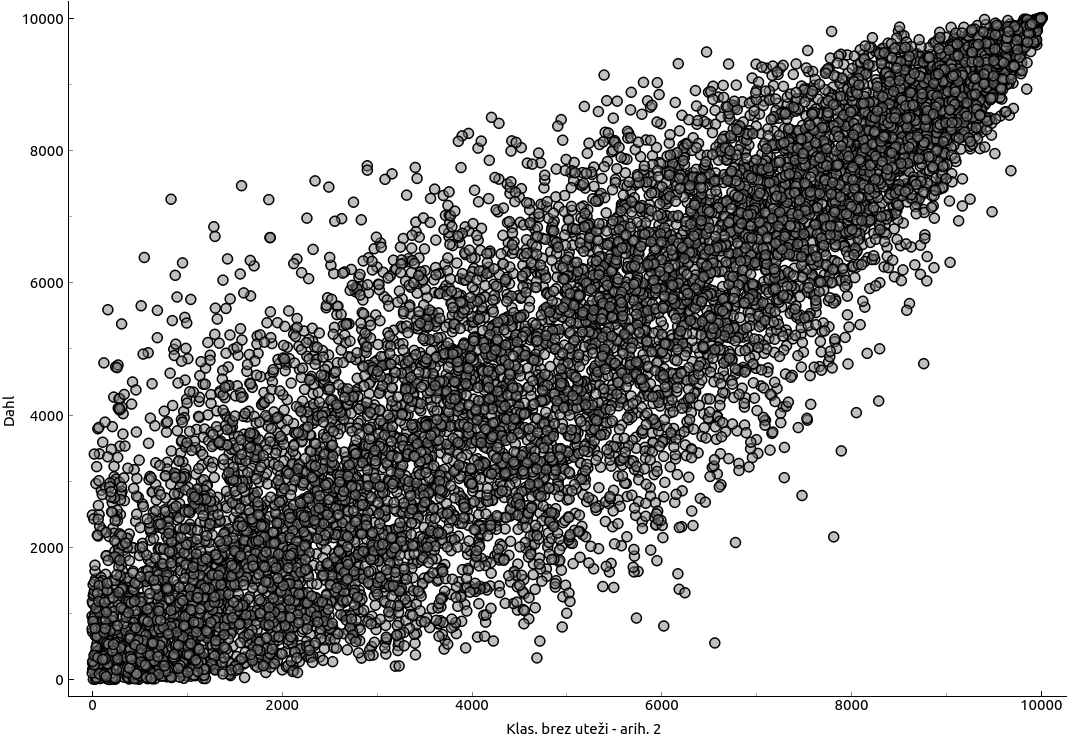
\includegraphics[width=6cm]{ranks_dahl_arh2}
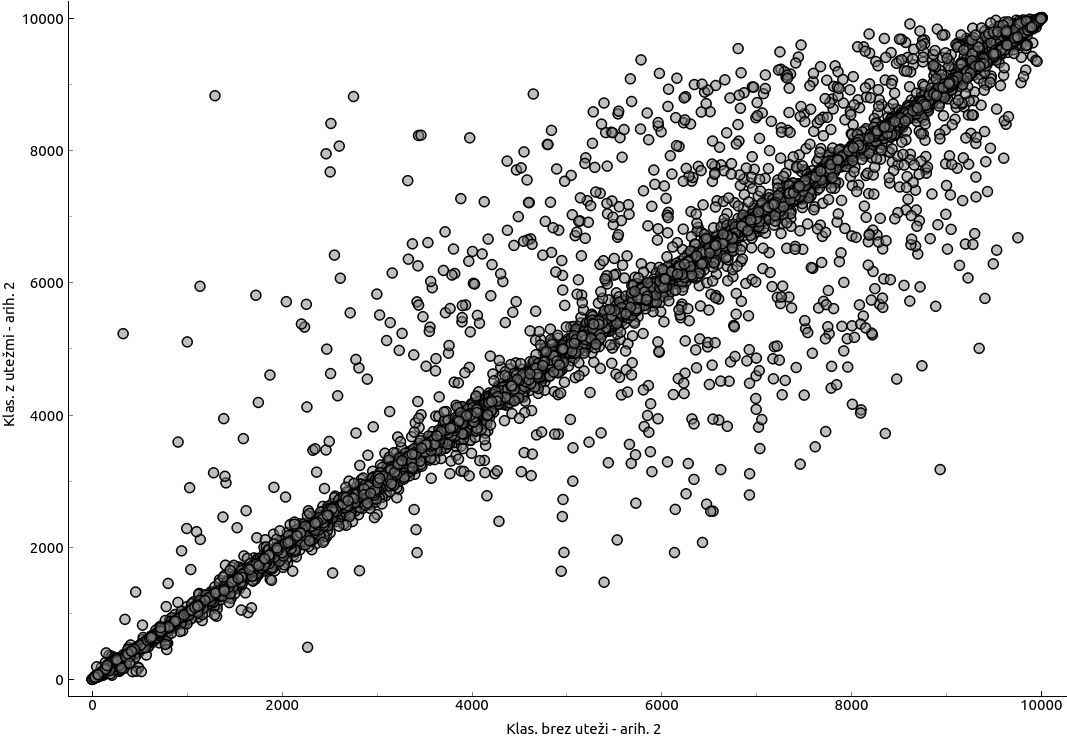
\includegraphics[width=6cm]{rank_arh2_arh2}
\end{center}
\caption{Graf prikazuje rangiranje slik glede na napako \textit{RMSE} pri dveh različnih metodah. $X$ os predstavlja rang pri prvi metodi, $Y$ pa rang pri drugi metodi. Prva slika prikazuje primerjave rangov Dahlove metode in klasifikacijske metode z arhitekture 2. Druga metoda prikazuje range pri dveh klasifikacijskih metodah z istimi arhitekturami.}
\label{im:ranks-between-methods}
\end{figure}

Ker smo želeli podobnost metod med seboj primerjati v prostoru, smo izračunali Spearmanovo korelacijo rangov \cite{hauke2011comparison} za vsak par metode. Korelacije so številčno prikazane v tabeli \ref{tab:spearman}. Za izris podobnosti smo uporabili metodo večdimenzionalno skaliranje (ang. {\em Multidimensional scaling} - MDS) \cite{Wickelmaier2003} na Spearmanivih korelacijah. 

Pristopi so glede na arhitekturo in vrsto pristopa razporejeni v prostor, ki je prikazan na sliki \ref{im:methods-mds}. Izkaže se, da se pristopi z klasifikacijo pojavijo desno v prostoru in so bolj oddaljeni od tistih z regresijo levo. Pri pristopih z klasifikacijo opazimo, da na različnost bolj vpliva vrsta arhitekture, kot uporaba uteži glede na pogostost barve. Izkaže se, da je pristop Zhang in sod. bližje tistim z globjo arhitekturo. Glede na to, da so lastnosti teh arhitektur popolnoma drugačne, se izkaže, da na podobnost glede na napake vpliva predvsem globina arhitekture. 

Pri regresijskih metodah lahko opazimo, da je največja razlika glede na uporabo globalne mreže. Pristopi, ki ne uporabljajo globalne mreže so na vrhu prikaza ostali pa spodaj. Regresija celotna slika VGG je nekje na sredini med obema gručama. To gre verjetno pripisati dejstvu, da ta pristop uporablja mrežo VGG-16, ki je del globalne mreže pri ostalih pristopih, vendar ta pristop to mrežo izkorišča kot glavno. 

Čeprav je Dahlov pristop glede na arhitekturo dosti podoben našim pristopom se glede na napake izkaže podoben pristopom brez globalne mreže. Pristop Iizuka in sod. je v gruči s pristopi, ki uporabljajo globalno mrežo, saj tudi sam uporablja podoben pristop. Pri pristopih z regresijo lahko opazimo še, da sta pristopa Iizuka in sod. ter pristop z regresijo na celi sliki bolj skupaj, saj oba delujeta na celotni sliki. 

\begin{figure}[htb]
\begin{center}
\centering
\fbox{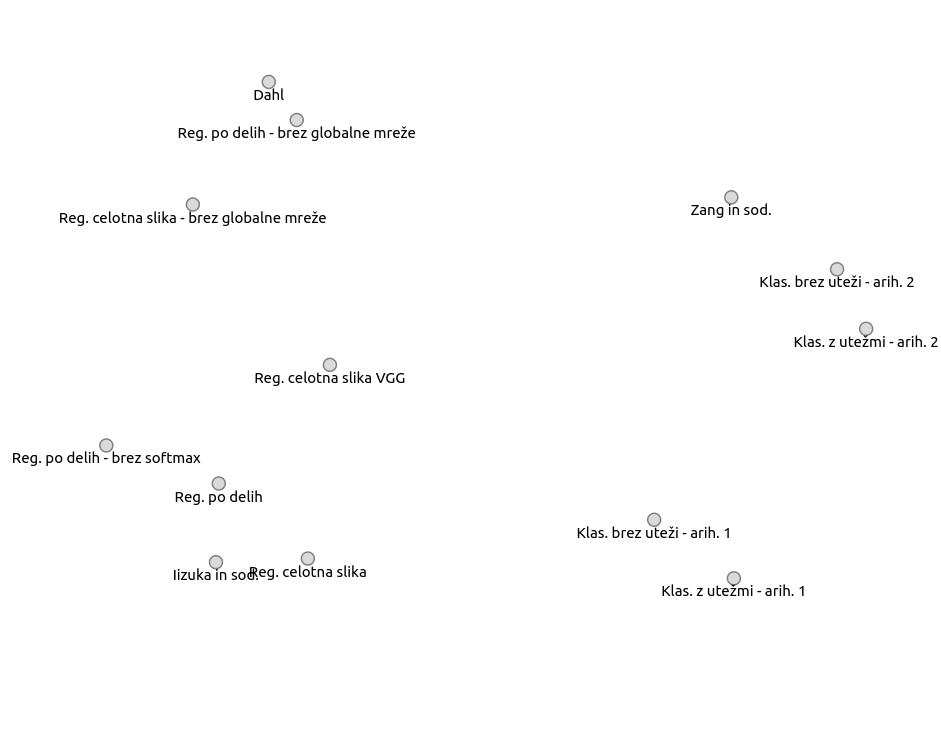
\includegraphics[width=12.5cm]{methods_mds}}
\end{center}
\caption{Primerjava metod v prostoru MDS kaže sorodnosti med metodami na način napovedovanja barve (klasifikacija proti regresiji) in glede na arhitekturo mreže. Mreže, ki uporabljajo mrežo VGG za napovedovanje objekta v sliki so bližje skupaj in modeli brez VGG mreže so bližje skupaj.  }
\label{im:methods-mds}
\end{figure}

Zanimalo nas je tudi. Katere so tiste slike, kjer eden od pristopov dobro obarva sliko, ostali pa mnogo slabše in obratno. Ob pogledu na sliko \ref{im:ranks-between-methods} lahko opazimo, da so taki primeri točke, ki ležijo najbolj stran od linearne premice, zato smo te slike našli z metodo za iskanje osamelcev (ang. {\em outliers}) \cite{Ramaswamy}. 

Slike, ki najbolj izstopajo glede na napako na različnih metodah, so prikazane kot točke v prostoru, ki ga dobimo z metodo MDS glede na napako, na sliki \ref{im:images-mds}. Ob pregledu slik se izkaže, da gre tukaj večinoma za slike, kjer je težje zaznati teksturo ob tem predvidevamo, da so se določene metode bolje naučile ravno te teksture kot druge. 

Ob bolj natančnem pregledu prostor smo ugotovili, da napaka močno povezana s motivom na sliki. V prostoru so bližje skupaj slike s podobnim motivom in barvami. Na levi strani so prikazane tri slike, ki so blizu skupaj in jim je skupno to, da je na sliki morje ali voda, ki sta oba modre barve in določen objekt (v našem primeru žival). Na desni strani sta dve slike, ki se tudi ujemata glede na odtenke v sliki, čeprav je motiv drugačen. 

\begin{figure}[htb]
\begin{center}
\centering
\fbox{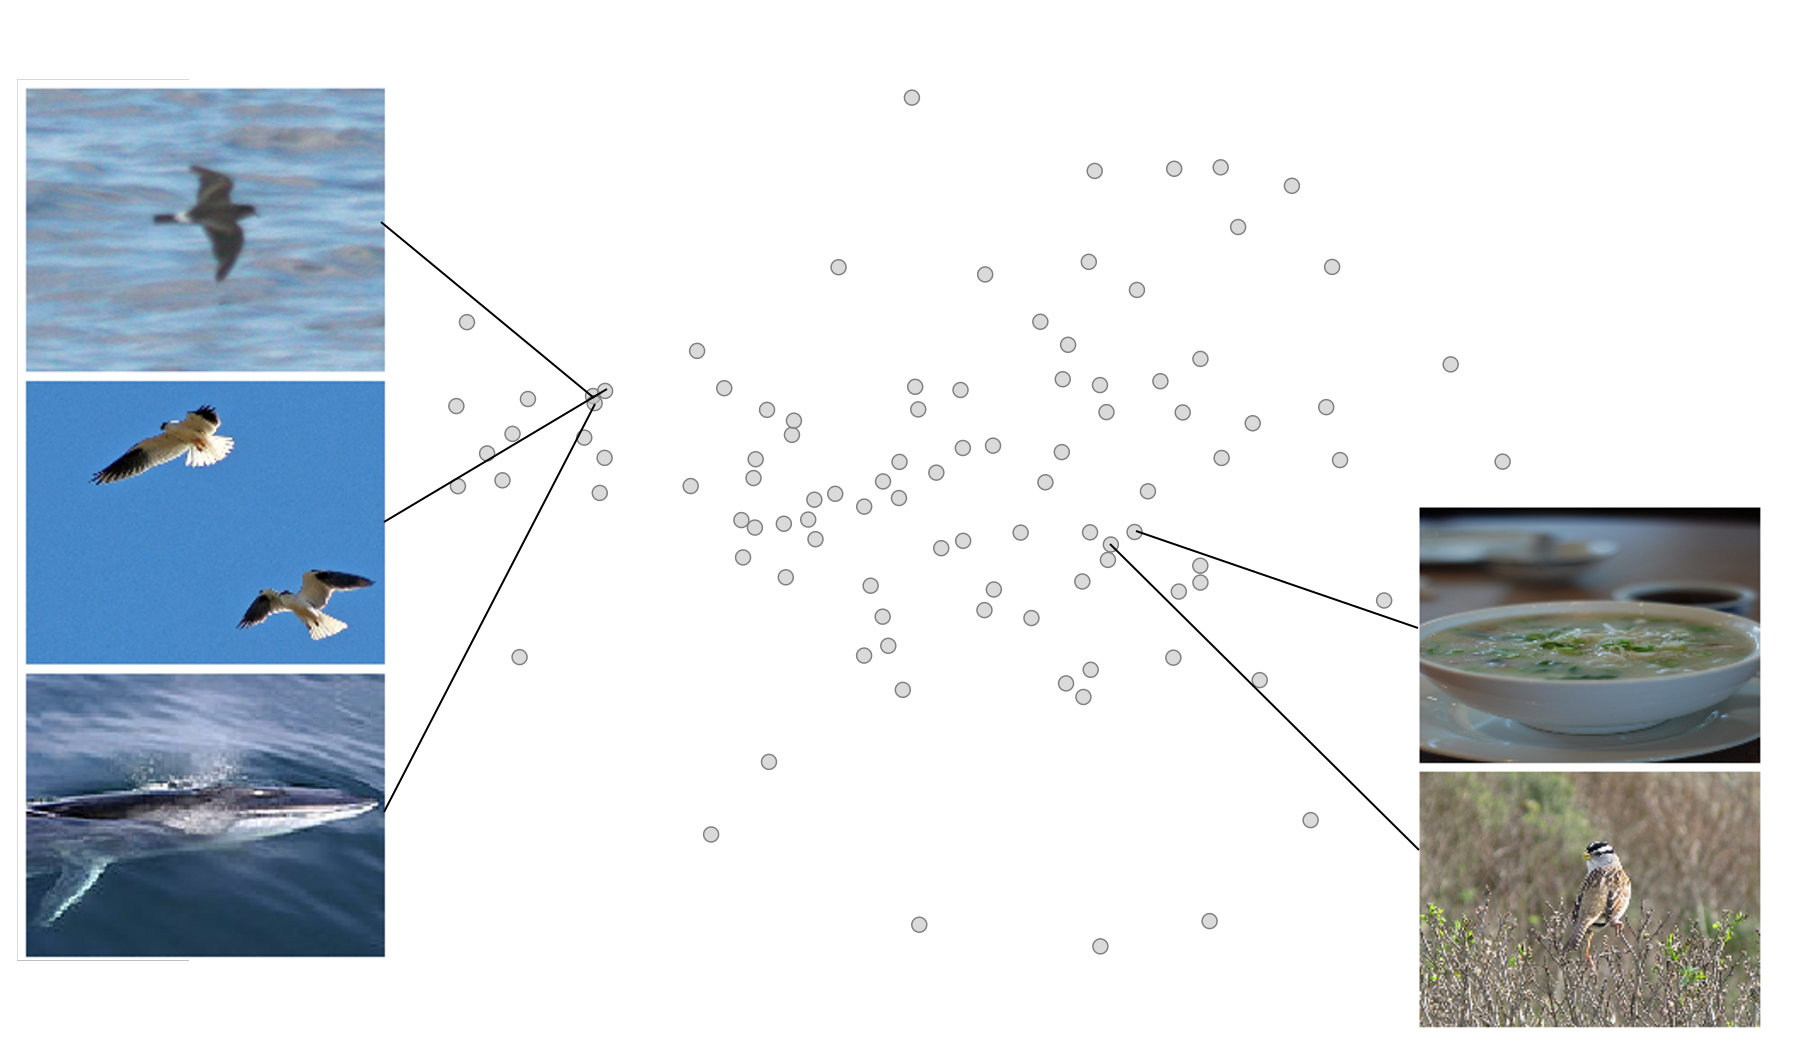
\includegraphics[width=11cm]{images_mds}}
\end{center}
\caption{Razporeditev slik v prostoru MDS, ki zajema 100 sli, ki kjer natančnosti najbolj odstopajo pri različnih metodah. V prostoru so točke podobnih slik bliže skupaj. Dve taki podobni skupini slik sta prikazani ob robu.   }
\label{im:images-mds}
\end{figure}

Ker pa se ukvarjamo s slikami pa dodajamo še primerjavo barvanja na slikah. Primerjave po pristopih so prikazane na sliki \ref{im:images-100-compare-reg} za regresijo in na sliki \ref{im:images-100-compare-klas} za klasifikacijo. Slike smo izbrali, tako da prva dva stolpca prikazujeta dve slike iz množice 20 najbolje obarvanih s strani vseh algoritmov, 3 in 4 stolpec prikazujeta slike, ki so se bile z različno dobro obarvane s strani različnih pristopov. Te slike sta izbrane izmed točk v prostoru na sliki \ref{im:images-mds}. Zadnja dva stolpca prikazujeta slike, ki so bile v množici 20 najslabše obarvanih s strani vseh algoritmov. 

Opazimo lahko, da sta slike v prvih dveh stolpcih v skupini najbolje obarvanih zato, ker so že originalne slike z zelo malo barve, te so namreč zelo blede. Algoritmi, posebej regresijskih, ki običajno obarvajo z bolj nenasičenimi barvami so se zato zelo približali originalni sliki, čeprav barvanje v več primerih ni ravno najboljše. Pri drugem in tretjem stolpcu so se nekateri pristopi dobro približali pravi barvi drugi se opazi, da barvanje s strani vseh algoritmov ni bilo enako dobro. Slike iz zadnjih dveh stolpcev sta bila glede na napako v množici najslabše obarvanih slik zato, ker imajo originalne slike zelo močne odtenke, katerim se pristopi niso približali, čeprav so nekatera barvanja dovolj naravna, če ne primerjamo z originalno sliko.

V primerjavi metod iz sorodnih del, pričakovano opazimo, da najboljše barva pristop Iizuka in sod., ki je imel tudi najmanjšo napako. Zang in sod. se na določenih delih obnese dobro, vendar so slike zelo lisaste in nepopolno obarvane, medtem ko so pri metodi Dahl odtenki zelo rjavi, čeprav vmes lahko opazimo nekaj pravih barv.

Pri primerjavi regresijskih metod lahko opazimo, da je po pričakovanjih najboljše barvanje s strani Regresije na celotnih sliki z globalno mrežo, čeprav Regresija na delih slik ne zaostaja dosti. Opazimo lahko tudi pomen in izboljšavo z uporabo globalne mreže. Enaki pristopi brez globalne mreže so obarvali bolj nenatančno, nenaravno, prisotnih je tudi več rjavih odtenkov. 

Pri klasifikacijskih pristopih opazimo, da pristopi z plitvo arhitekturo dajo boljše rezultate, kot tisti z globoko, kjer barvanja skoraj da ni. Pri primerjavi z utežmi in brez lahko zaznamo, da pristop z utežmi barva z močnejšimi odtenki, kot tisti brez, kar je bilo za pričakovati, saj je namen uteži, zmanjšati izbor bolj šibkejših odtenkov, ki imajo $a*$ in $b*$ vrednost bližje nič. Pristopi so nagnjeni k izbiri teh, ker se bolj pogosto pojavljajo v slikah. Kljub barvanju z močnejši odtenki barv in s tem približevanju realni barvi, je na pogled barvanje brez uteži bolj naravno, saj je opaziti manj napak v barvanju (na sliki s ptico sta les in ptica pobarvan bolj realno in letalo nima okoli sivinskega pasu).

Pri primerjavi slik pristopi z regresijo obarvajo bolje in bolj naravno, kot pristopi z klasifikacijo, čeprav je nekaj izjem pri barvanju neba in praproti. Izkaže se tudi, da barvanje z regresijo  večkrat obarva z bolj rjavimi odtenki, kar pri klasifikacijskih pristopih ni zaznati. Tam je bolj pogosto, da slika ni obarvana. 


\begin{figure}[htb]
\begin{center}
\centering
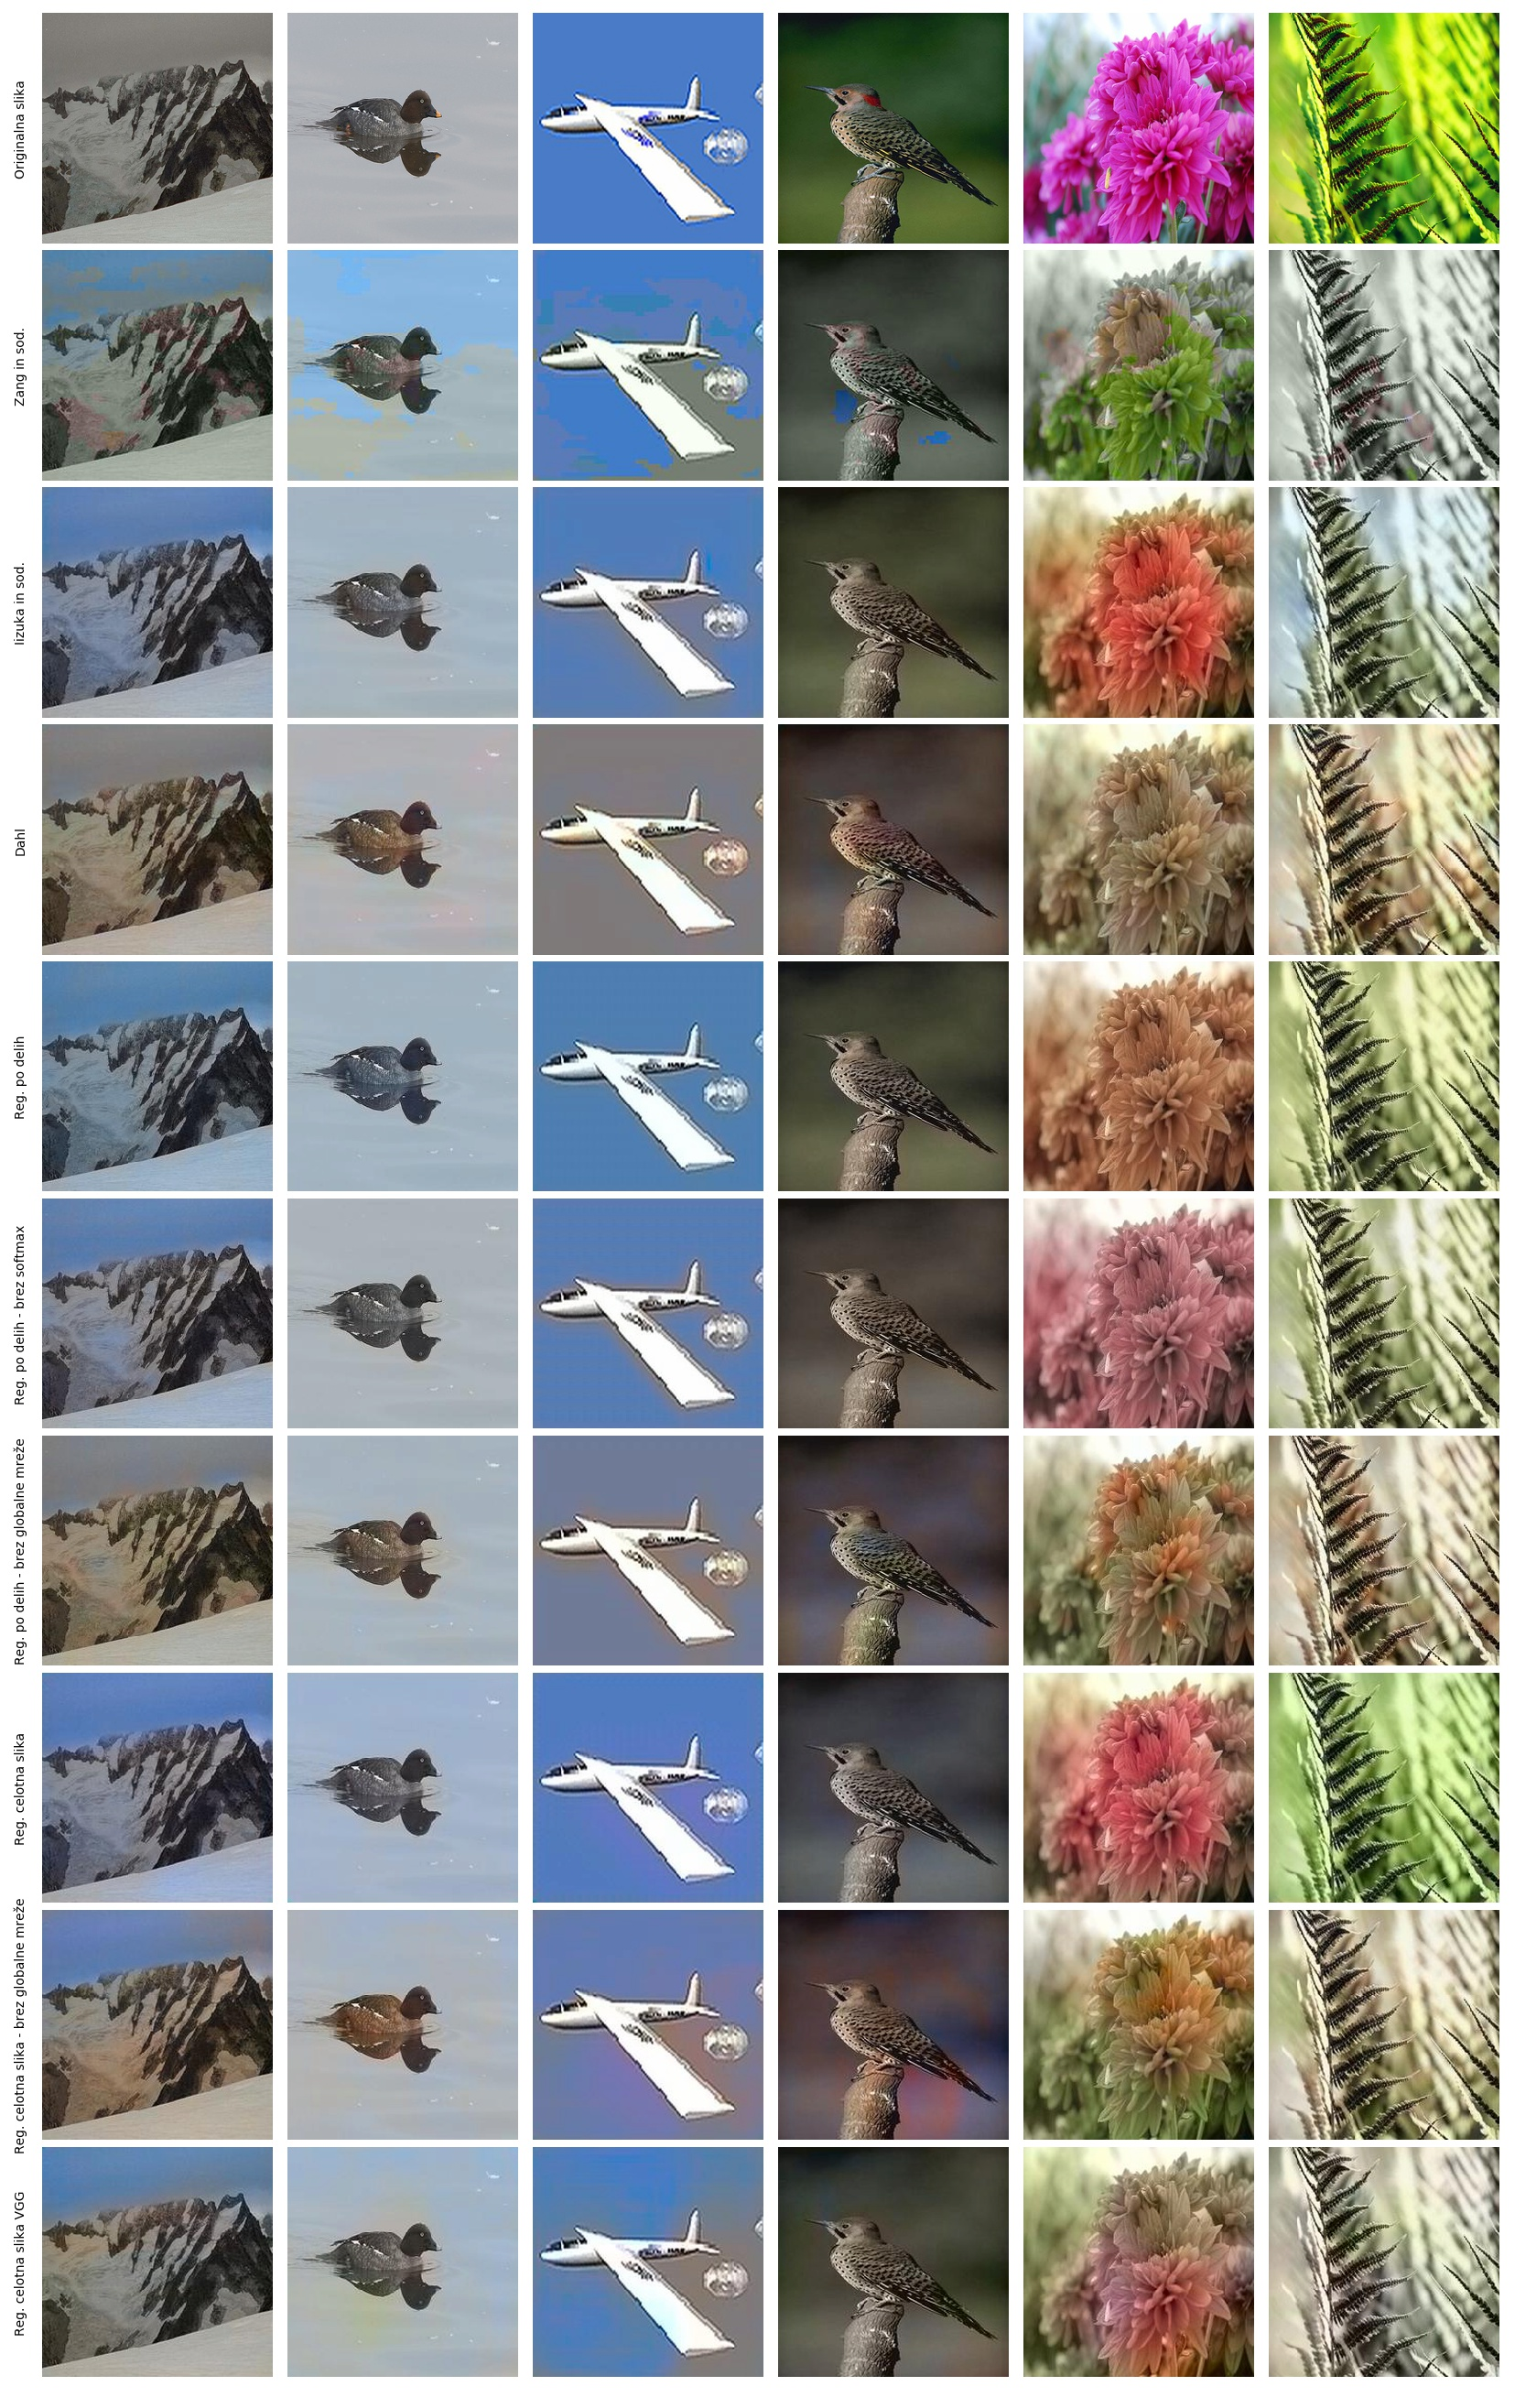
\includegraphics[width=11.5cm]{images-methods-comparison-100-reg}
\end{center}
\caption{Slike iz testne množice, ki so bile obarvane z regresijskimi pristopi opisanimi v tem delu in pristopi iz sorodnih del. Vsaka vrstica prikazuje drugo metodo, prva vrstica prikazuje originalno sliko.}
\label{im:images-100-compare-reg}
\end{figure}

\begin{figure}[htb]
\begin{center}
\centering
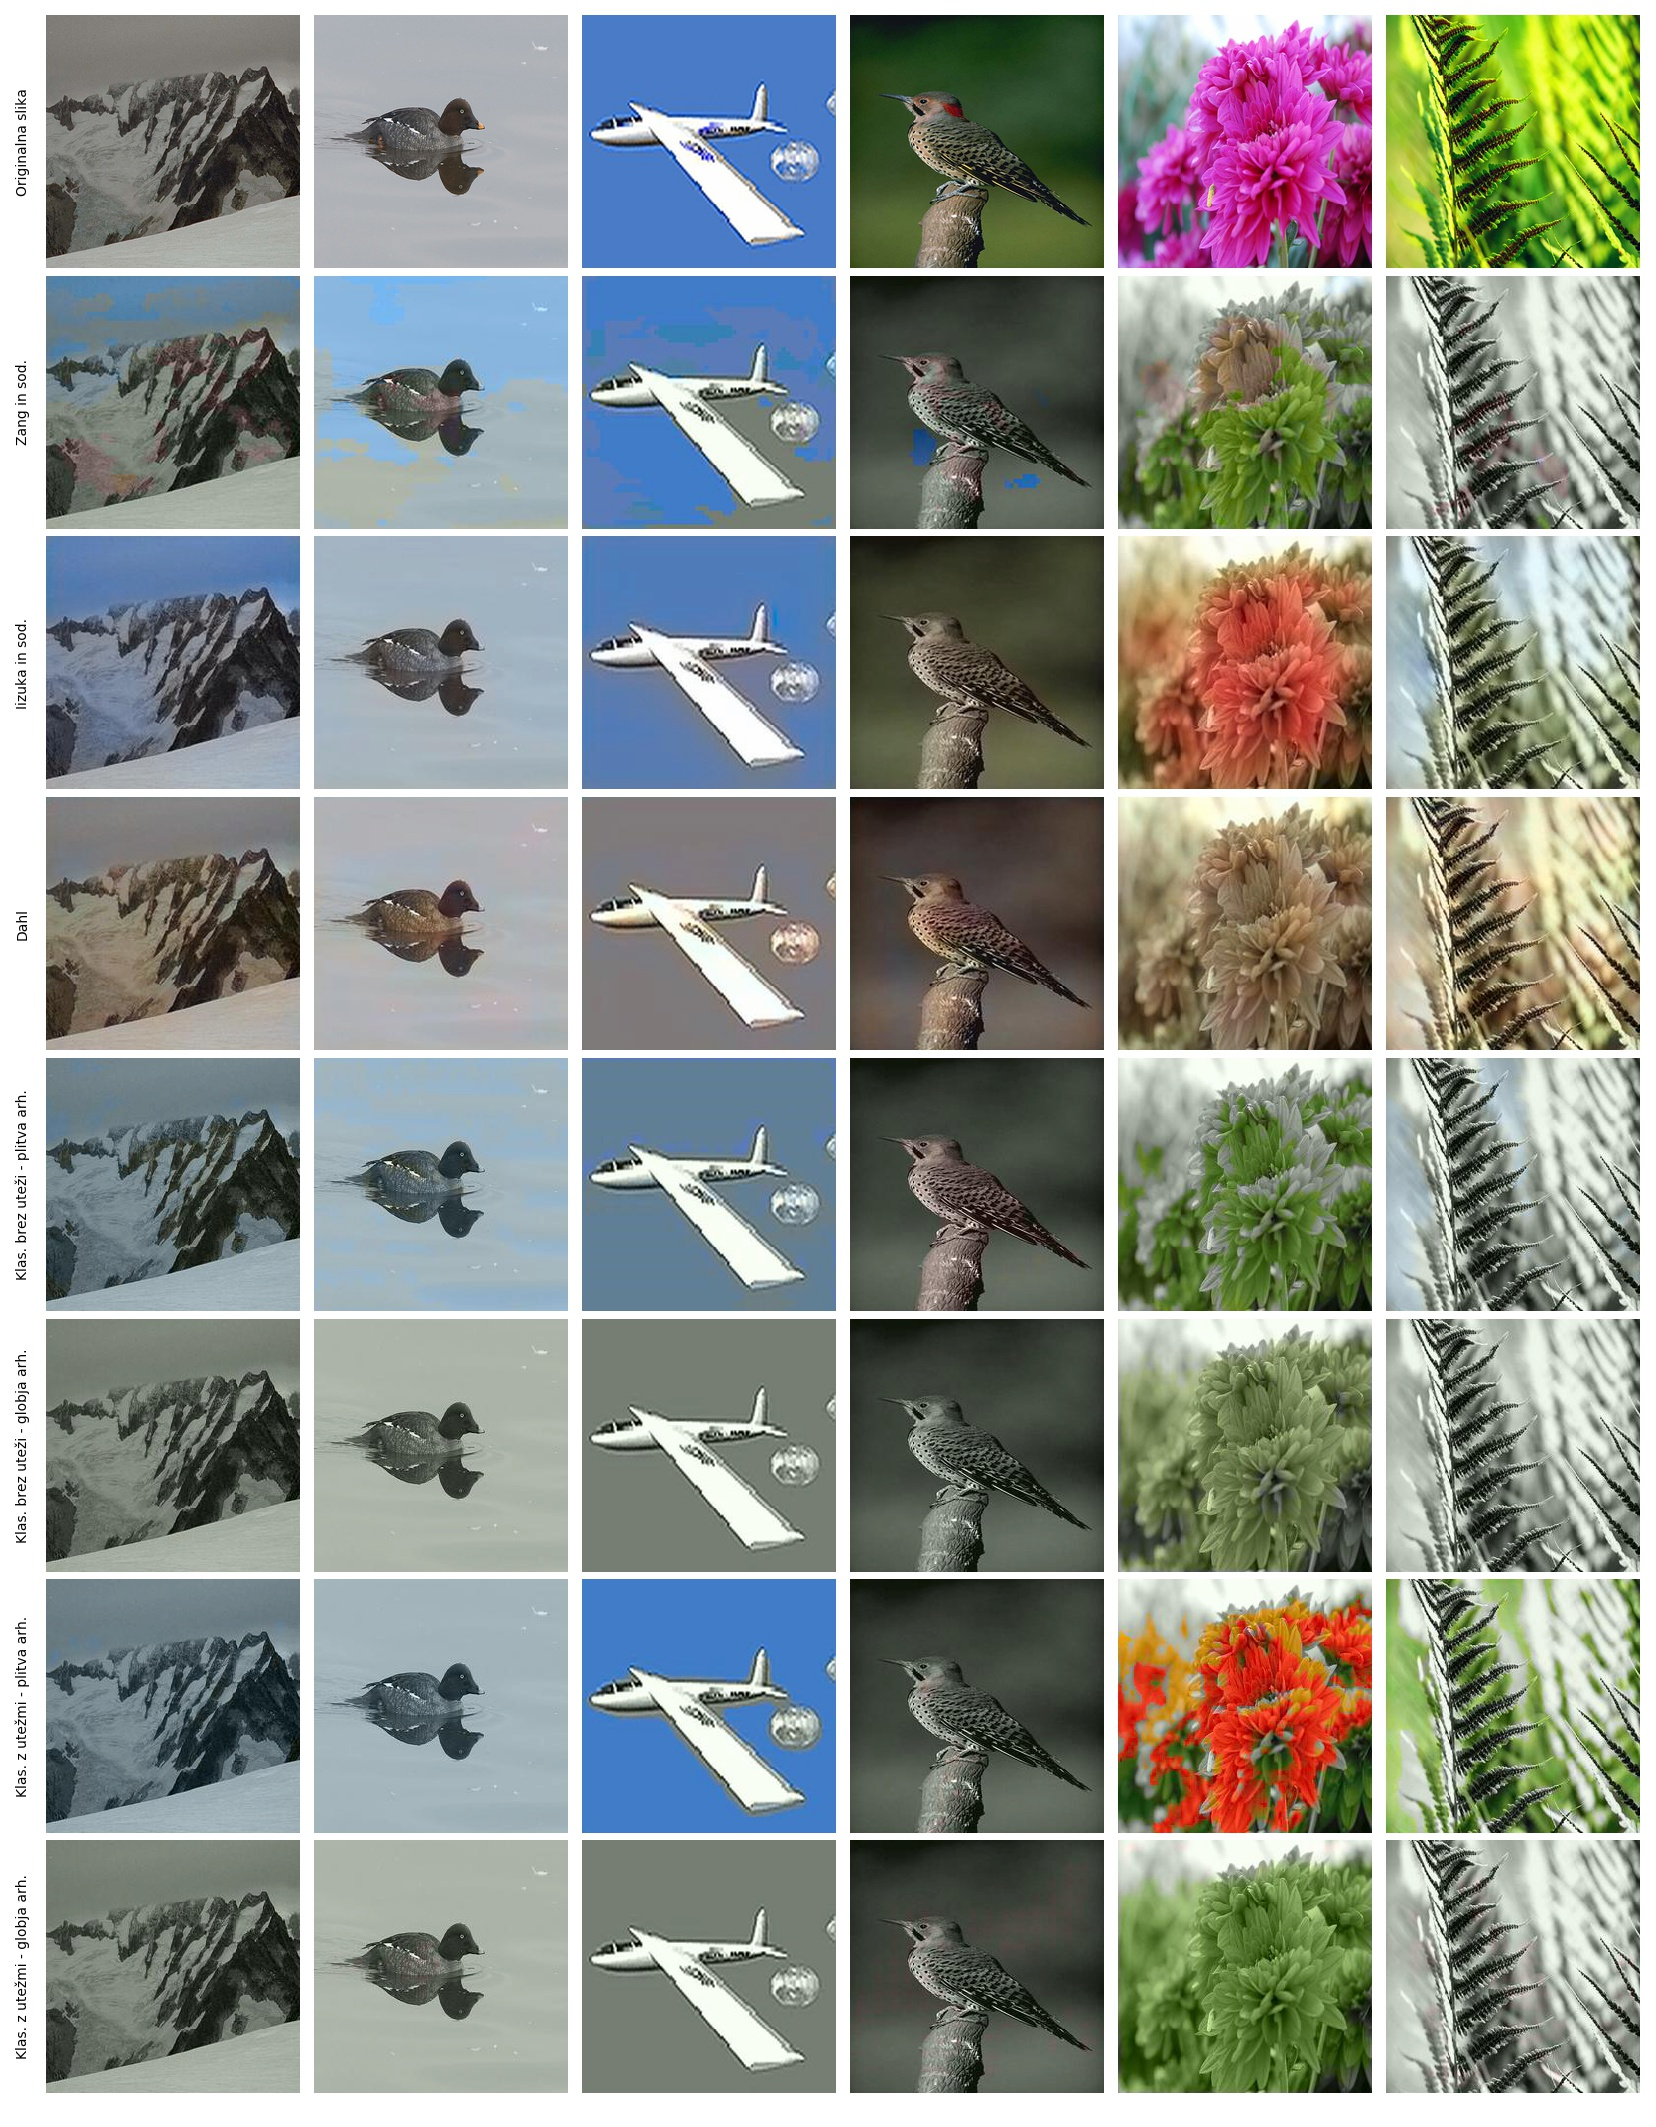
\includegraphics[width=11.5cm]{images-methods-comparison-100-klas}
\end{center}
\caption{Slike iz testne množice, ki so bile obarvane z k pristopi opisanimi v tem delu in pristopi iz sorodnih del. Vsaka vrstica prikazuje drugo metodo, prva vrstica prikazuje originalno sliko. }
\label{im:images-100-compare-klas}
\end{figure}


\section{Primerjava metod na večji učni množici}

Tukaj bi primerjali metode, ki bi bile naučene na več slikah, tako bi pridobili tudi boljša barvanja za pokazat izboljševanje barvanja glede na epoche. Primerjavo bi izvedli na manj manj metodah. 

\section{Barvanje večjih slik}

Tabela \ref{tab:vecjih} prikazuje napake pri dveh velikostih slik na dveh metodah. Ena velikost je velikost na kateri je bila mreža naučena, druga pa je večja velikost slik. Izkaže se, da ima pristop \textit{Regresija po delih z globalno mrežo} zelo majhno razliko v napaki, pri barvanju slik večjih velikosti glede na napako na osnovni velikosti, medtem ko je ta razlika pri pristopu Iizuka in sod. merjena v RMSE kar $6.18$. 

\begin{table}[htb]
\caption{Primerjava napak pristopov Iizuka in sod. ter \textit{regresija po delih z globalno mrežo} pri barvanju večjih slik. Za računaje napake so uporabljene metrike opisane v poglvaju \ref{ch:napake}.}
\begin{center}
\begin{tabular}{l|ccc}
Pristop & Velikost slik & RMSE & PSNR \\
\hline
\multirow{2}{*}{Iizuka in sod.} & 224 & 10.018 & 24.750 \\
 								& 896 & 16.136 & 20.906 \\
\hline
\multirow{2}{*}{Reg. po delih} & 224 & 9.892 & 24.700 \\
 								& 896 & 10.096 & 24.523 \\
 

\end{tabular}
\end{center}
\label{tab:vecjih}
\end{table}

% TODO: dodaj se slike

%----------------------------------------------------------------
% Poglavje (Chapter) 6: Zaključek
%----------------------------------------------------------------

\chapter{Zaključek}


%----------------------------------------------------------------
% Poglavje: Priloge
%----------------------------------------------------------------

\appendix
%\addcontentsline{toc}{chapter}{Razširjeni povzetek}
\chapter{Spearmanova korelacija rangov med metodami}

\begin{table}
\caption{Spearmanova korelacija med metodami. }
\begin{center}
\begin{tabular}{l|ccccccccccccc}
          &Zang&Iizuka&Dahl      &Reg. po de&Reg. po de&Reg. po de&Reg. celot&Reg. celot&Reg. celot&Klas. brez&Klas. brez&Klas. z ut&Klas. z ut \\
\hline
Zang in so&1.0000    &0.8607    &0.8688    &0.8637    &0.8407    &0.8898    &0.8779    &0.8804    &0.8969    &0.9092    &0.9409    &0.9242    &0.9023     \\
Iizuka in &0.8607    &1.0000    &0.8936    &0.9454    &0.9420    &0.9015    &0.9472    &0.9206    &0.9398    &0.9012    &0.8519    &0.8535    &0.8889     \\
Dahl      &0.8688    &0.8936    &1.0000    &0.9008    &0.9058    &0.9816    &0.8889    &0.9518    &0.9196    &0.8636    &0.8861    &0.8722    &0.8431     \\
Reg. po de&0.8637    &0.9454    &0.9008    &1.0000    &0.9440    &0.9096    &0.9392    &0.9149    &0.9309    &0.9004    &0.8622    &0.8578    &0.8861     \\
Reg. po de&0.8407    &0.9420    &0.9058    &0.9440    &1.0000    &0.9120    &0.9313    &0.9194    &0.9211    &0.8795    &0.8434    &0.8390    &0.8640     \\
Reg. po de&0.8898    &0.9015    &0.9816    &0.9096    &0.9120    &1.0000    &0.9005    &0.9642    &0.9263    &0.8784    &0.8979    &0.8817    &0.8582     \\
Reg. celot&0.8779    &0.9472    &0.8889    &0.9392    &0.9313    &0.9005    &1.0000    &0.9140    &0.9334    &0.9030    &0.8657    &0.8632    &0.8904     \\
Reg. celot&0.8804    &0.9206    &0.9518    &0.9149    &0.9194    &0.9642    &0.9140    &1.0000    &0.9371    &0.8759    &0.8650    &0.8558    &0.8544     \\
Reg. celot&0.8969    &0.9398    &0.9196    &0.9309    &0.9211    &0.9263    &0.9334    &0.9371    &1.0000    &0.9065    &0.8881    &0.8831    &0.8937     \\
Klas. brez&0.9092    &0.9012    &0.8636    &0.9004    &0.8795    &0.8784    &0.9030    &0.8759    &0.9065    &1.0000    &0.9209    &0.9240    &0.9489     \\
Klas. brez&0.9409    &0.8519    &0.8861    &0.8622    &0.8434    &0.8979    &0.8657    &0.8650    &0.8881    &0.9209    &1.0000    &0.9813    &0.9126     \\
Klas. z ut&0.9242    &0.8535    &0.8722    &0.8578    &0.8390    &0.8817    &0.8632    &0.8558    &0.8831    &0.9240    &0.9813    &1.0000    &0.9230     \\
Klas. z ut&0.9023    &0.8889    &0.8431    &0.8861    &0.8640    &0.8582    &0.8904    &0.8544    &0.8937    &0.9489    &0.9126    &0.9230    &1.0000     \\
\end{tabular}
\end{center}
\label{tab:spearman}
\end{table}

\chapter{Podrobnosti arhitektur}

\begin{longtable}[h]{l|ccccc}
\caption{Tabela prikazuje nivoje plitve arhitekture z globalno mrežo in njihove parametre. $K$ predstavlja število kanalov izhoda nevronske mreže, $J$ pove velikost jedra, $Ko$ je korak (ang. {\em stride}) uporabljen na nivoju in $Akt$ predstavlja aktivacijo po vsakem nivoju. Zadnji konvolucijski nivo nima definiranega števili izhodnih kanalov, saj je to odvisno od pristopa, ki smo ga uporabili. Pri nadvzorčenju smo vedno nadvzorčili s faktorjem 2, kar pomeni, da ima tensor, ki predstavlja izhod po širini in višini dvakratno velikost. }\\

		Nivo & K & J & K & Akt \\
		\hline
		Vhod & 1 & - & - & - \\
		2D konvolucija & 64 & 3 & 2 & Relu\\
		2D konvolucija & 128 & 3 & 1 & Relu \\
		2D konvolucija & 128 & 3 & 2 & Relu \\
		2D konvolucija & 256 & 3 & 1 & Relu\\		
		2D konvolucija & 256 & 3 & 2 & Relu\\
		2D konvolucija & 512 & 3 & 1 & Relu\\
		2D konvolucija & 512 & 3 & 1 & Relu\\
		2D konvolucija & 256 & 3 & 1 & Relu\\
		Združitev z globalno mrežo & 512 & - & - & - \\

		2D konvolucija & 256 & 3 & 1 & Relu\\
		Nadvzorčenje & 256 & - & - & -\\
		2D konvolucija & 256 & 3 & 1 & Relu\\
		2D konvolucija & 256 & 3 & 1 & Relu\\
		Nadvzorčenje & 256 & - & - & -\\
		2D konvolucija &  & 3 & 1 & Relu \\
        

\label{tab:arh1}
\end{longtable}

\begin{longtable}[h]{ll|ccccc}
\caption{Tabela prikazuje nivoje globje arhitekture z globalno mrežo in njihove parametre. $K$ predstavlja število kanalov izhoda nevronske mreže, $J$ pove velikost jedra, $Ko$ je korak (ang. {\em stride}) uporabljen na nivoju, $Akt$ predstavlja aktivacijo po vsakem nivoju in $Reg$ določa stopnjo regularizacije. V vseh nivojih uporabljamo \textit{L2 regulrizacijo} \cite{mackay1992practical}. Zadnji konvolucijski nivo nima definiranega števili izhodnih kanalov, saj je to odvisno od pristopa, ki smo ga uporabili. }\\

Zap. št. & Nivo & K & J & Ko & Akt & Reg\\
\hline
0 & Vhod & 1 & - & - & - & - \\
1 & 2D konvolucija & 64 & 3 & 1 & Relu & 0.01\\

2 & Maks. združevanje & 64 & 2 & 2 & - & - \\
3 & 2D konvolucija & 128 & 3 & 1 & Relu & 0.01\\
4 & 2D konvolucija & 128 & 3 & 1 & Relu & 0.01\\
5 & 2D konvolucija & 128 & 3 & 1 & Relu & 0.01\\
6 & Vsota z 3 & 128 & - & - & - & -\\
7 & 2D konvolucija & 128 & 3 & 1 & Relu & 0.01\\

8 & Maks. združevanje & 128 & 2 & 2 & - & - \\
9 & 2D konvolucija & 256 & 3 & 1 & Relu & 0.01\\
10 & 2D konvolucija & 256 & 3 & 1 & Relu & 0.01\\
11 & 2D konvolucija & 256 & 3 & 1 & Relu & 0.01\\
12 & Vsota z 9 & 256 & - & - & - & -\\
13 & 2D konvolucija & 256 & 3 & 1 & Relu & 0.01\\
		
14 & Maks. združevanje & 265 & 2 & 2 & - & - \\
15 & 2D konvolucija & 512 & 3 & 1 & Relu & 0.01\\
16 & 2D konvolucija & 512 & 3 & 1 & Relu & 0.01\\
17 & 2D konvolucija & 512 & 3 & 1 & Relu & 0.01\\
18 & Vsota z 15 & 512 & - & - & - & -\\
19 & 2D konvolucija & 512 & 3 & 1 & Relu & 0.01\\
20 & 2D konvolucija & 256 & 3 & 1 & Relu & 0.01\\

21 & Združitev z globalno mrežo & 512 & - & - & - & - \\

22 & 2D konvolucija & 128 & 3 & 1 & Relu & 0.01\\
23 & 2D transponirana kovnolucija & 64 & 3 & 2 & Relu & 0.01\\
24 & 2D kovnolucija & 64 & 3 & 1 & Relu & 0.01 \\
25 & 2D kovnolucija & 64 & 3 & 1 & Relu & 0.01 \\
		
26 & 2D transponirana kovnolucija & 64 & 3 & 2 & Relu & 0.01\\
27 & 2D kovnolucija & 32 & 3 & 1 & Relu & 0.01 \\
28 & 2D kovnolucija &  & 3 & 1 & Relu & 0.01 \\

\label{tab:arh2}
\end{longtable}

\begin{longtable}[h]{ll|ccccc}
\caption{Tabela prikazuje nivoje dopolnjene VGG mreže in njihove parametre. $K$ predstavlja število kanalov izhoda nevronske mreže, $J$ pove velikost jedra, $Ko$ je korak (ang. {\em stride}) uporabljen na nivoju, $Akt$ predstavlja aktivacijo po vsakem nivoju in $Reg$ določa stopnjo regularizacije. V vseh nivojih uporabljamo \textit{L2 regulrizacijo} \cite{mackay1992practical}. Zadnji konvolucijski nivo nima definiranega števili izhodnih kanalov, saj je to odvisno od pristopa, ki smo ga uporabili. Vsako nadvzorčenje prostorske dimenzije poveča za 2 krat.  }\\

Zap. št. & Nivo & K & J & Ko & Akt & Reg\\
\hline
0 & Vhod & 1 & - & - & - & - \\
1 & VGG-16 mreža & 512 & - & - & - & -\\

2 & Nadvzorčenje & 512 & - & - & - & - \\
3 & 2D konvolucja & 256 & 3 & 1 & Relu & 0.01 \\
4 & 2D konvolucja & 256 & 3 & 1 & Relu & 0.01 \\

5 & Nadvzorčenje & 256 & - & - & - & - \\
6 & 2D konvolucja & 128 & 3 & 1 & Relu & 0.01 \\
7 & 2D konvolucja & 128 & 3 & 1 & Relu & 0.01 \\

8 & Nadvzorčenje & 128 & - & - & - & - \\
9 & 2D konvolucja & 64 & 3 & 1 & Relu & 0.01 \\
10 & 2D konvolucja & 164 & 3 & 1 & Relu & 0.01 \\

11 & Nadvzorčenje & 64 & - & - & - & - \\
12 & 2D konvolucja & 32 & 3 & 1 & Relu & 0.01 \\
13 & 2D konvolucja &  & 3 & 1 & Relu & 0.01 \\

\label{tab:arh4}
\end{longtable}




%----------------------------------------------------------------
% SLO: bibliografija
% ENG: bibliography
%----------------------------------------------------------------
\bibliographystyle{elsarticle-num}

%----------------------------------------------------------------
% SLO: odkomentiraj za uporabo zunanje datoteke .bib (ne pozabi je potem prevesti!)
% ENG: uncomment to use .bib file (don't forget to compile it!)
%----------------------------------------------------------------
\bibliography{bibliography}

%----------------------------------------------------------------
% SLO: zakomentiraj spodnji del, če uporabljaš zunanjo .bib datoteko
% ENG: comment the part below if using the .bib file
%----------------------------------------------------------------



\end{document}
